%! TEX program = xelatex
%% \documentclass[letterpaper,nonstop,draftmode]{simplethesisdissertation}
\documentclass[12pt,twoside]{report}
%!TEX root = ./Thesis.tex
\usepackage{breakcites}
\usepackage{amsmath,amssymb}
\usepackage{amsfonts}
\usepackage{mathtools}

\usepackage{blindtext} % Package to generate dummy text throughout this template 

%%%%%%%%%%%%%%%%%% FONT CHOICE %%%%%%%%%%%%%%%%%%%%%%

% \usepackage{unicode-math}
\usepackage[bold-style=ISO]{unicode-math}
\usepackage{parskip}
\defaultfontfeatures{Scale=MatchLowercase}
\setmainfont{TeX Gyre Pagella}[Scale = 1.0]

% \setmathfont{Pagella Math}
% \setmathfont{XITS Math}
\usepackage{bm}

% \renewcommand{\boldsymbol}{\symbf} % this is because unicode-math with the bold-style option wants you to use \symbf rather that \boldsymbol, for some reason

% \linespread{1.05} % Line spacing - Palatino needs more space between lines

%%%%%%%%%%%%%%%%%% END FONT CHOICE %%%%%%%%%%%%%%%%%%%%%%

\usepackage{xspace} % to avoid newcommand eating trailing space
\usepackage{etoolbox}
\usepackage{microtype} % Slightly tweak font spacing for aesthetics

\usepackage[english]{babel} % Language hyphenation and typographical rules

\usepackage[hmarginratio=1:1,top=32mm,columnsep=20pt]{geometry} % Document margins
\usepackage{marginnote}
\renewcommand*{\marginfont}{\color{blue}\itshape\footnotesize}
\usepackage{setspace} % provides \setstretch
\usepackage[small,labelfont=bf,up,textfont=it,up]{caption} % Custom captions under/above floats in tables or figures
\usepackage{subcaption}
\usepackage{booktabs} % Horizontal rules in tables
\usepackage{fullpage}

\usepackage{lettrine} % The lettrine is the first enlarged letter at the beginning of the text

\usepackage{enumitem} % Customized lists
\setlist[itemize]{noitemsep} % Make itemize lists more compact


\usepackage{acronym}
\newacro{AD}{Automatic Differentiation}
\newacro{DR}{Dimensionality Reduction}
\newacro{ML}{Machine Learning}
\newacro{NN}{Neural Network}
\newacro{PCA}{Principal Component Analysis}
\newacro{CNN}{Convolutional Neural Network}
\newacro{SGD}{Stochastic Gradient Descend}
\newacro{SVM}{Support Vector Machine}
\newacro{QFT}{Quantum Fourier Transform}
\newacro{QML}{Quantum Machine Learning}

\newacro{QW}{Quantum Walk}
\newacro{DTQW}{Discrete-Time Quantum Walk}
\newacro{CTQW}{Continuous-Time Quantum Walk}

\newacro{LG}{Laguerre-Gauss}
\newacro{CCD}{Charge Coupled Device}
\newacro{SLM}{Spatial Light Modulator}
\newacro{SAM}{Spin Angular Momentum}
\newacro{OAM}{Orbital Angular Momentum}
\newacro{QWP}{Quarter-wave Plate}
\newacro{HWP}{Half-wave Plate}
\newacro{VVB}{Vector Vortex Beam}
\newacro{PBS}{Polarising Beamsplitter}
\newacro{QP}{Q-Plate}
\newacro{SMF}{Single Mode Optical Fiber}
\newacro{APD}{Avalanche Photodiode}
\newacro{SCS}{Spin Coherent State}
\newacro{SPDC}{Spontaneous Parametric Down Conversion}
\newacro{PPKTP}{Periodically-Poled Potassium Titanyl Phosphate}

\usepackage{todonotes}

\usepackage{abstract} % Allows abstract customization
\renewcommand{\abstractnamefont}{\normalfont\bfseries} % Set the "Abstract" text to bold
\renewcommand{\abstracttextfont}{\normalfont\small\itshape} % Set the abstract itself to small italic text

% \usepackage{titlesec} % Allows customization of titles
% \renewcommand\thesection{\Roman{section}} % Roman numerals for the sections
% \renewcommand\thesubsection{\roman{subsection}} % roman numerals for subsections
% \titleformat{\section}[block]{\large\scshape\centering}{\thesection.}{1em}{} % Change the look of the section titles
% \titleformat{\subsection}[block]{\large}{\thesubsection.}{1em}{} % Change the look of the section titles

% \usepackage{fancyhdr} % Headers and footers
% \pagestyle{fancy} % All pages have headers and footers
% \fancyhead{} % Blank out the default header
% \fancyfoot{} % Blank out the default footer
% \fancyhead[C]{Running title $\bullet$ May 2016 $\bullet$ Vol. XXI, No. 1} % Custom header text
% \fancyfoot[RO,LE]{\thepage} % Custom footer text

\usepackage{titling} % Customizing the title section

\usepackage{physics}
\usepackage{siunitx}

\usepackage{csquotes}

\usepackage{easyReview}

\usepackage{graphicx}
\graphicspath{{./Figures/}{./Figures/gate-learning/}{./Figures/quantum-walks/}{./Figures/VVBs/}}
\usepackage{wrapfig}
% \usepackage{subfig}

\usepackage{placeins}  % provides \FloatBarrier

\usepackage{xcolor}
\usepackage{nameref}
\usepackage[colorlinks=true,citecolor=red]{hyperref}
\usepackage[nameinlink]{cleveref}
\crefname{appsec}{Appendix}{Appendices}

\usepackage{listings} % for code snippets
\definecolor{codegreen}{rgb}{0,0.6,0}
\definecolor{codegray}{rgb}{0.5,0.5,0.5}
\definecolor{codepurple}{rgb}{0.58,0,0.82}
\definecolor{backcolour}{rgb}{0.95,0.95,0.92}
 
\lstdefinestyle{mystyle}{
    backgroundcolor=\color{backcolour},
    commentstyle=\color{codegreen},
    keywordstyle=\color{magenta},
    numberstyle=\tiny\color{codegray},
    stringstyle=\color{codepurple},
    basicstyle=\ttfamily\scriptsize,
    breakatwhitespace=false,
    breaklines=true,
    captionpos=b,
    keepspaces=true,
    numbers=left,
    numbersep=5pt,
    showspaces=false,
    showstringspaces=false,
    showtabs=false,
    tabsize=2
} 
\lstset{style=mystyle}


\usepackage{tikz}

\usepackage{amsthm}
% \newtheorem{example}{Example}

\usepackage[many]{tcolorbox}
% \tcbuselibrary{theorems}
% \newtcbtheorem
%   [number within=section]% init options
%   {example}% name
%   {Example}% title
%   {%
%     breakable, enhanced,
%     colback=green!5,
%     colframe=green!35!black,
%     fonttitle=\bfseries,
%     title={Porco dio}
%   }% options
%   {example}% prefix
\newtcolorbox[
    auto counter,
    number within=section,
    crefname={example}{examples}
]{example}[1][]{
  enhanced,
  breakable,
%   colback=green!5,
%   colframe=green!35!black,
  fonttitle=\bfseries,
  title={Example \thetcbcounter},
  #1
}

\newtcolorbox[
    auto counter,
    number within=section,
    crefname={example}{examples}
]{examplebox}[2][]{
  enhanced,
  breakable,
  fonttitle=\bfseries,
  title={Example \thetcbcounter: #2},
  #1
}

\newtcolorbox[auto counter]{tbox}[2][]{%
	enhanced,% float*=t,
	colback=gray!5!white, colframe=gray!75!black,
	width=\textwidth,
	title={Box \thetcbcounter: #2}, #1
}


% \usepackage[
%     backend=biber,
%     style=alphabetic,
%     maxcitenames=1,
%     url=true,
%     doi=true,
%     sorting=ynt,
%     backref=true
% ]{biblatex}
% \DeclareNameAlias{author}{given-family}

\usepackage{breakcites}
\usepackage[
    backend=biber,
    style=authoryear,
    maxnames=1,
    url=false,
    doi=true,
    sortcites=true,
    sorting=ynt,
    backref=true,
    firstinits=false,
    uniquename=false,
    natbib
]{biblatex}
\renewcommand{\cite}{\parencite}

% -------------- START AUTHORYEAR FIX
% \usepackage{twoopt}
% \usepackage{ifthen}

% \newcommand\black[1]{\textcolor[rgb]{0,0,0}{#1}}

% \newcommandtwoopt{\mycitet}[3][aa][bb]{%
%     \ifthenelse{\equal{#1}{aa}}                                                                         % if nargin == 1
%       {\hyperlink{cite.#3}{\citeauthor{#3} \black{(}\citeyear{#3}\black{)}}}                            %     \citet{key}
%       {\ifthenelse{\equal{#2}{bb}}                                                                      % elseif nargin == 2
%         {\hyperlink{cite.#3}{\citeauthor{#3} \black{(}\citeyear{#3}\black{,}~#1\black{)}}}              %     \citet[pg]{key}
%         {\ifthenelse{\equal{#1}{}}                                                                      % elseif #1 = []
%           {\hyperlink{cite.#3}{\citeauthor{#3} \black{(}\citeyear{#3}\black{,}~#2\black{)}}}            %     \citet[][pg]{key}
%           {\ifthenelse{\equal{#2}{}}                                                                    % elseif #2 == []
%             {\hyperlink{cite.#3}{\citeauthor{#3} \black{(#1~}\citeyear{#3}\black{)}}}                   %     \citet[eg][]{key}
%             %                                                                                           % else
%             {\hyperlink{cite.#3}{\citeauthor{#3} \black{(#1~}\citeyear{#3}\black{,}~#2\black{)}}}       %     \citet[eg][pg]{key}}
%           }
%         }
%       }
% }

% \makeatletter 
% \newcommand{\multicite}[1]{% taken from egreg, see link
%   \@tempswafalse
%   \@for\next:=#1\do
%     {\if@tempswa;~\else\@tempswatrue\fi
%     \hyperlink{cite.\next}{\citeauthor{\next}\black{,~}\citeyear{\next}}%
%     }%
% }
% \makeatother

% \newcommandtwoopt{\mycitep}[3][aa][bb]{%        
%     \ifthenelse{\equal{#1}{aa}}                                                                  % if nargin == 1
%       {(\multicite{#3})}                                                                         %    \citep{key(s)}
%       {\ifthenelse{\equal{#2}{bb}}                                                               % elseif nargin == 2
%           {(\hyperlink{cite.#3}{\citeauthor{#3}\black{,~}\citeyear{#3}\black{,~}#1})}            %    \citep[pg]{key}
%           {\ifthenelse{\equal{#1}{}}                                                             % elseif #1 = []
%               {(\hyperlink{cite.#3}{\citeauthor{#3}\black{,~}\citeyear{#3}\black{,~}#2})}        %    \citep[][pg]{key}
%               {\ifthenelse{\equal{#2}{}}                                                         % elseif #2 == []
%                   {(#1~\multicite{#3})}                                                          %    \citep[eg][]{key(s)}
%                   %                                                                              % else
%                   {(#1~\hyperlink{cite.#3}{\citeauthor{#3}\black{,~}\citeyear{#3}\black{,~}#2})} %    \citep[eg][pg]{key}}
%               }
%            }
%       }
% }
% ------------------- END AUTHORYEAR FIX

% ---------------- START SECOND FIX
% Just for demo
\ExecuteBibliographyOptions{maxcitenames=1}

\DeclareFieldFormat{citehyperref}{%
  \DeclareFieldAlias{bibhyperref}{noformat}% Avoid nested links
  \bibhyperref{#1}}

\DeclareFieldFormat{textcitehyperref}{%
  \DeclareFieldAlias{bibhyperref}{noformat}% Avoid nested links
  \bibhyperref{%
    #1%
    \ifbool{cbx:parens}
      {\bibcloseparen\global\boolfalse{cbx:parens}}
      {}}}

\savebibmacro{cite}
\savebibmacro{textcite}

\renewbibmacro*{cite}{%
  \printtext[citehyperref]{%
    \restorebibmacro{cite}%
    \usebibmacro{cite}}}

\renewbibmacro*{textcite}{%
  \ifboolexpr{
    ( not test {\iffieldundef{prenote}} and
      test {\ifnumequal{\value{citecount}}{1}} )
    or
    ( not test {\iffieldundef{postnote}} and
      test {\ifnumequal{\value{citecount}}{\value{citetotal}}} )
  }
    {\DeclareFieldAlias{textcitehyperref}{noformat}}
    {}%
  \printtext[textcitehyperref]{%
    \restorebibmacro{textcite}%
    \usebibmacro{textcite}}}

% \renewcommand{\baselinestretch}{1.2}
% \setlength{\parskip}{\smallskipamount}
% \setlength{\parindent}{0pt}
% ---------------- END SECOND FIX


\addbibresource{Thesis.bib}


% \newcommand{\bs}[1]{\pmb{#1}}
\newcommand{\bs}[1]{\symbf{#1}}
\newcommand{\on}[1]{\operatorname{#1}}
\newcommand{\ansatz}{Ansatz }

\newcommand{\bsx}{{\bs{x}}}
\newcommand{\bsw}{{\bs{w}}}
\newcommand{\bslambda}{{\bs{\lambda}}}
\newcommand{\bstheta}{{\bs{\theta}}}
\renewcommand{\grad}{\nabla}

\newcommand{\calA}{{\mathcal{A}}}
\newcommand{\calC}{{\mathcal{C}}}
\newcommand{\calE}{{\mathcal{E}}}
\newcommand{\calF}{{\mathcal{F}}}
\newcommand{\calG}{{\mathcal{G}}}
\newcommand{\calH}{{\mathcal{H}}}
\newcommand{\calO}{{\mathcal{O}}}
\newcommand{\calP}{{\mathcal{P}}}
\newcommand{\calS}{{\mathcal{S}}}
\newcommand{\calU}{{\mathcal{U}}}
\newcommand{\calW}{{\mathcal{W}}}
\newcommand{\calV}{{\mathcal{V}}}

\newcommand{\calHcoin}{{\calH_\calC}}
\newcommand{\calHwalker}{{\calH_\calS}}

\newcommand{\CC}{{\mathbb{C}}}
\newcommand{\EE}{{\mathbb{E}}}
\newcommand{\HH}{{\mathbb{H}}}
\newcommand{\NN}{{\mathbb{N}}}
\newcommand{\PP}{{\mathbb{P}}}
\newcommand{\QQ}{{\mathbb{Q}}}
\newcommand{\RR}{{\mathbb{R}}}
\newcommand{\ZZ}{{\mathbb{Z}}}

\newcommand{\tildePP}{\tilde{\PP}}

\newcommand{\UToff}{\calU_{\on{Toff}}}
\newcommand{\HToff}{\calH_{\on{Toff}}}
\newcommand{\HPrimeToff}{\calH'_{\on{Toff}}}
\newcommand{\HTildeToff}{\tilde{\calH}_{\on{Toff}}}

\newcommand{\UFred}{\calU_{\Fred}}
\newcommand{\Fred}{\on{Fred}}
\newcommand{\HFred}{\calH_{\Fred}}
\newcommand{\HTildeFred}{\tilde{\calH}_{\Fred}}
\newcommand{\HPrimeFred}{\calH'_{\Fred}}

\newcommand{\CNOT}{\on{CNOT}}
\newcommand{\Toff}{\on{Toff}}

\newcommand{\spanR}{\on{Span}_{\RR}}

\renewcommand{\Re}{\on{Re}}
\renewcommand{\Im}{\on{Im}}
\DeclareMathOperator*{\argmax}{arg\,max}
\DeclareMathOperator*{\argmin}{arg\,min}
\DeclareMathOperator*{\Prob}{Prob}

\newcommand{\barcalF}{\overline{\calF}}
\newcommand{\Lin}{\on{Lin}}

\newcommand{\tmpHeading}[1]{\textbf{\color{orange}\textit{(#1)}}}


\newcommand\scalemath[2]{\scalebox{#1}{\mbox{\ensuremath{\displaystyle #2}}}}

% checkmark symbol
\usepackage{bbding}
\newcommand{\ccheck}{\color{red}{\Checkmark}}

%%%%%%%%%%%%%%%%%%%%%%%%%%%%%%%%%%%%%%%%%%%%%%%%%%%%%%%%%%%%%%%%%
%% PREAMBLE.
%%%%%%%%%%%%%%%%%%%%%%%%%%%%%%%%%%%%%%%%%%%%%%%%%%%%%%%%%%%%%%%%%

% Document properties.
\def\DocumentTitle{Machine-learning-assisted state and gate engineering for quantum technologies}
\def\AuthorName{Luca Innocenti}

% PDF settings and properties.
\hypersetup{
pdftitle={\DocumentTitle},
pdfauthor={\AuthorName},
pdfsubject={Ph.D. Thesis, Queen's University Belfast, 2019},
pdfcreator={XeLaTeX},
pdfproducer={},
pdfkeywords={},
unicode=true,
% bookmarks=true,
bookmarksopen=true,
pdfstartview=FitH,
pdfpagelayout=OneColumn,
pdfpagemode=UseOutlines,
hidelinks,
breaklinks,
bookmarksnumbered
}
\hypersetup{
  colorlinks   = true, %Colours links instead of ugly boxes
  urlcolor     = green!80!black, %Colour for external hyperlinks
  linkcolor    = blue, %Colour of internal links 	q
  citecolor    = red!80!black %Colour of citations
}

% Accent colors.
\definecolor{AccentOne}{RGB}{0,68,186} % blue

%%%%%%%%%%%%%%%%%%%%%%%%%%%%%%%%%%%%%%%%%%%%%%%%%%%%%%%%%%%%%%%%%
%% ACTUAL DOCUMENT.
%%%%%%%%%%%%%%%%%%%%%%%%%%%%%%%%%%%%%%%%%%%%%%%%%%%%%%%%%%%%%%%%%

\begin{document}

%!TEX root = ./Thesis.tex

% Use Roman numerals (i, ii, iii, etc.) for page numbers in the front matter.
\pagenumbering{roman}

%%%%%%%%%%%%%%%%%%%%%%%%%%%%%%%%%%%%%%%%%%%%%%%%%%%%%%%%%%%%%%%%%
%% TITLE PAGE.
%%%%%%%%%%%%%%%%%%%%%%%%%%%%%%%%%%%%%%%%%%%%%%%%%%%%%%%%%%%%%%%%%

% No headers or footers on the title page.
\thispagestyle{empty}

\begingroup
\centering
\setstretch{1.0}
~
\\[1em]
\sffamily\bfseries\fontsize{26}{31.2}\selectfont
\DocumentTitle
% \\
% Use Manual Line Breaks If Necessary
\\[0.4in]
\normalfont\large
Thesis by
\\[0.25em]
\sffamily\bfseries\Large
\AuthorName
\\[0.4in]
\normalfont\normalsize
In Partial Fulfillment of the Requirements
\\[0.5em]
for the Degree of
\\[0.5em]
Doctor of Philosophy
\\[0.5em]
in
\\[0.5em]
Physics
\vfill
% \includegraphics[height=1.8in]
% {Figure-SchoolLogo}
% \\[1.5em]
Queen's University Belfast
\\[0.5em]
Belfast, UK
\\[1.5em]
2020
\\[0.5em]
(Defended \emph{\textbf{who knows when}})
\par
\endgroup

\clearpage

%%%%%%%%%%%%%%%%%%%%%%%%%%%%%%%%%%%%%%%%%%%%%%%%%%%%%%%%%%%%%%%%%
%% COPYRIGHT PAGE.
%%%%%%%%%%%%%%%%%%%%%%%%%%%%%%%%%%%%%%%%%%%%%%%%%%%%%%%%%%%%%%%%%

\pagestyle{plain}
\setcounter{page}{2}

\begingroup
\centering
\setstretch{1.0}
\null
\vfill
{\sffamily\textcopyright}~2016
\\[0.5em]
\AuthorName
\\[0.5em]
All Rights Reserved
\par
\endgroup

\clearpage

%%%%%%%%%%%%%%%%%%%%%%%%%%%%%%%%%%%%%%%%%%%%%%%%%%%%%%%%%%%%%%%%%
%% DEDICATION PAGE.
%%%%%%%%%%%%%%%%%%%%%%%%%%%%%%%%%%%%%%%%%%%%%%%%%%%%%%%%%%%%%%%%%

% \begingroup
% \centering
% \setstretch{1.0}
% ~
% \\[1in]
% \textit{Insert dedication here}
% \par
% \endgroup

\clearpage

%%%%%%%%%%%%%%%%%%%%%%%%%%%%%%%%%%%%%%%%%%%%%%%%%%%%%%%%%%%%%%%%%
%% ACKNOWLEDGMENTS.
%%%%%%%%%%%%%%%%%%%%%%%%%%%%%%%%%%%%%%%%%%%%%%%%%%%%%%%%%%%%%%%%%

\chapter*{Acknowledgments}
\addcontentsline{toc}{chapter}{Acknowledgments}

\clearpage

%%%%%%%%%%%%%%%%%%%%%%%%%%%%%%%%%%%%%%%%%%%%%%%%%%%%%%%%%%%%%%%%%
%% ABSTRACT.
%%%%%%%%%%%%%%%%%%%%%%%%%%%%%%%%%%%%%%%%%%%%%%%%%%%%%%%%%%%%%%%%%

\chapter*{Abstract}
\addcontentsline{toc}{chapter}{Abstract}

In this Thesis, we discuss applications of machine learning to quantum information science.
The interface between these two fields has been the subject of much research, recently, driven by the many successes of machine learning for diverse pattern recognition tasks. The work reported in this Thesis addresses precisely the potential of such an interdisciplinary line of research and illustrates how machine learning provides a valuable add-on to standard techniques used in the context of quantum technologies.

Specifically, we will first study the problem of devising time-independent dynamics implementing target quantum operations.
This involves a challenging optimisation task, which is hard to tackle with standard numerical tools.
We demonstrate how the use of supervised learning algorithms can dramatically speed-up this task.

We then consider the tasks of engineering and characterising quantum states in large Hilbert spaces. Motivated by strong experimental reasons, we consider explicitly the embodiment of such multi-dimensional quantum systems provided by the orbital angular momentum and polarisation degrees of freedom of light.
We devise a protocol involving quantum walks to implement arbitrary states by only making use of the possibility to couple polarisation and orbital angular momentum through relatively recent technological advances in the field of linmear optics.
This protocol relies solely on the properties of quantum walk dynamics, and is therefore applicable to different types of architectures.

We then present an experimental demonstration of this engineering strategy, and consider the issue of assessing the quality of the states thus generated.
We show how different machine learning algorithms, including supervised and unsupervised learning ones, are able to tackle this problem and provide useful information in realistic experimental conditions.


\clearpage

%%%%%%%%%%%%%%%%%%%%%%%%%%%%%%%%%%%%%%%%%%%%%%%%%%%%%%%%%%%%%%%%%
%% TABLE OF CONTENTS (TOC), LISTS OF FIGURES, TABLES, ETC.
%%%%%%%%%%%%%%%%%%%%%%%%%%%%%%%%%%%%%%%%%%%%%%%%%%%%%%%%%%%%%%%%%

\tableofcontents

% \listoffigures

% \listoftables

\clearpage

% Use Arabic numerals (1, 2, 3, etc.) for subsequent page numbers.
\pagenumbering{arabic}


%!TEX root = ./Thesis.tex

\chapter{Introduction}
\label{chapter:introduction}

\section{Quantum information science}

\tmpHeading{What is quantum information?}
Quantum information science can be defined as the study of how information behaves, and can be manipulated, at the quantum level~\cite{nielsen2006quantum,watrous2018theory}.
The reasons for studying this are many-fold. On the one hand, quantum mechanics challenged our previously naive way of understanding how information behaves, showing us how the standard rules of probability theory cease to apply in some regimes.
On the other hand, from a more practical point of view, there is much to gain from such a deeper understanding of how information can be manipulated. Indeed, so much of the modern age relying on the capability to manipulate ever vaster heaps of data, it is only natural that insights telling us that quantum physics allows to process information dramatically faster than what classical computers are capable of would gain so much traction.
Furthermore, quantum information does not just hold the promise of faster information processing, but can also be exploited to devise new and improved means of communication, via faster and more secure communication protocols enabled by the properties of quantum entanglement~\cite{gisin2002quantum,krenn2016quantum,pirandola2019advances}.
Among the many approaches explored in the course of the last century, the most notable areas of research fall, broadly speaking, under the names of quantum computation~\cite{shor1997polynomial,steane1998quantum,ladd2010quantum}, quantum simulation~\cite{lloyd1996universal,georgescu2014quantum,koch2019quantum}, quantum communication~\cite{bennett1993teleporting}, and quantum cryptography~\cite{bennett2014quantum}.


\tmpHeading{Quantum computing}
Ever since Feynman first proposed a way to \emph{exploit} the peculiarities of quantum mechanics to solve classical hard problems~\cite{feynman1982simulating}, more and more research has been devoted into trying to understand exactly why and how quantum mechanics can provide advantages for information processing.
In fact, the realisation itself that this was possible at all prompted a shift of interest into a broad variety of research directions focussed on applying quantum mechanics to build better technologies. This has by some being named a \textit{second quantum revolution}~\cite{dowling2003quantum}, to differentiate it from the \emph{first quantum revolution}, which was when people first realised in the early 19th century how quantum mechanics could be used to explain known phenomena \highlight{is this paragraph really needed?}.
Among the other technologies, quantum computers are arguably the idea that received the most traction in recent years, possibly due to the monopolising prominence of their classical cousins.
Still, the dream of practical and useful quantum computation remains far on the horizon, and arguably still requires a fair number of theoretical and technological breakthroughs to be achieved~\cite{preskill2018quantum,flamini2018photonic,wang2019integrated}.
Nonetheless, the last few years have seen a number of such breakthroughs follow one another~\cite{fowler2012surface,barends2014superconducting,córcoles2015demonstration,ofek2016extending,arute2019quantum}.
Moreover, even though achieving scalable and fault-tolerant large-scale quantum computation remains a titanic challenge with present-day technology, there are ways to at least settle the overarching question of whether it is possible \textit{even in principle} to solve problems faster than what classical physics allows~\cite{aaronson2011computational,bremner2016average,boixo2018characterizing,aaronson2017complexity,neill2018blueprint}. This spurred the race to achieve the so-called \textit{quantum computational supremacy}~\cite{broome2012photonic,spring2012boson,crespi2013integrated,tillmann2013experimental,bentivegna2015experimental,zhong201812photon,zhong2019experimental,wang2019boson,bouland2018complexity,arute2019quantum}.
Several architectures are being studied as possible physical media for quantum information processing, including schemes relying on photonics~\cite{wang2019integrated,flamini2018photonic}, trapped ions~\cite{bruzewicz2019trappedion,lekitsch2017blueprint}, superconducting~\cite{krantz2019quantum,you2011atomic}, or cold atoms.
Similarly, many paradigms have been developed. One broad distinction can be made between \textit{discrete variables}~\cite{walmsley2005applied,andersen2015hybrid} and \textit{continuous variables}~\cite{lloyd1999quantum,braunstein2005quantum} approaches.
On top of this, several different paradigms are possible, ranging from the more commonly familiar notion of the circuit model for quantum computation~\cite{nielsen2006quantum}, to one-way quantum computation approaches~\cite{raussendorf2001one,walther2005experimental,browne2006one}, to adiabatic quantum computing~\cite{aharonov2004adiabatic,albash2018adiabatic}.

\tmpHeading{How are we connected to the problems in quantum computing?}
In this thesis, we will concern ourselves with problems that, while not directly related to the issues of actually building or programming a quantum computer, are about some of the many ancillary problems that arise in dealing with quantum devices and quantum information processing in general.
In particular, the problem of devising dynamics resulting in target operations between a set of qubits -- which will be referred to as the \emph{quantum gate learning problem} here -- is the topic of~\cref{chapter:gate_learning}; the problem of how to generate target quantum states -- often referred to as \emph{quantum state engineering} -- is discussed in~\cref{chapter:quantum_walks,chapter:experimental_engineering_qudits}; finally,~\cref{chapter:ML_VVBs} deals with the issue of reconstructing the properties of quantum states from experimental data.
\highlight{(sta frase nun me piace)}

\section{Machine learning and quantum physics}
\label{sec:intro:ML}

\tmpHeading{Machine learning}
Parallel to the surge of interest in quantum technologies, another field of study that has recently seen an explosion of funding and research is \ac{ML}~\cite{friedman2001elements,you2011atomic,bishop2006pattern,abu2012learning,murphy2012machine,mehta2019highbias}.
Roughly speaking, \ac{ML} refers to a class of algorithms whose goal is to learn from, and make predictions about, data.
Despite~\ac{ML} encompassing a wide variety of problems and techniques, the underlying conceptual framework can be understood as that of finding a set of parameters $\bstheta$ such that the corresponding map $f_\bstheta:\bs x\mapsto f_\bstheta(\bs x)$ fits the dataset under consideration, for some choice of \emph{model} $\bstheta\mapsto f_\bstheta$.
For example, in a \emph{classification problem}, $\bs x$ will be a set of real vectors, and $f_\bstheta(\bs x)$ can only have a finite number of values (for example, if we want to classify a set of images as representing ``cats'' or ``dogs'', $f_\bstheta(\bs x)\in\{\text{cat},\text{dog}\}$).

\tmpHeading{Just glorified curve-fitting?}
From this point of view, \ac{ML} algorithms might appear to be no different than simple fitting algorithms, and it is indeed not rare to hear people say that ``\emph{machine learning is just glorified curve-fitting}''. While there is some truth in such a statement, in the sense that both ``naive curve fitting'' and ``machine learning tasks'' can be unified under a single conceptual framework, such statements are completely off the mark when their implied meaning is to undersell the field of \ac{ML}.
Indeed, the ``simple'' problem of ``fitting a model'' to a given dataset, when no further assumptions are made over the type of data and model, is such a generic and hard problem that vastly different techniques and ideas are required to handle it in different circumstances.

\tmpHeading{``Quantum machine learning''?}
In particular, the intersection of \ac{ML} and quantum information science is also currently under intense study, and falls generically under the name of \ac{QML}~\cite{wittek2014quantum,schuld2014introduction,adcock2015advances,biamonte2017quantum}.
Due to the wide reach of both fields, \ac{QML} inevitably branched out into several different directions of study.
The terminology of was first used to refer to quantum algorithms tackling \ac{ML} tasks more efficiently~\cite{giovannetti2008quantum,harrow2009quantum,lloyd2013quantum,lloyd2014quantum,rebentrost2014quantum,lloyd2016quantum,rebentrost2018quantum,rebentrost2016quantum}. This line of study can therefore be considered as a subfield of quantum computation and quantum algorithm development focussed on the task of big data processing. An important body of work followed this path~\cite{wittek2014quantum,schuld2014introduction,dunjko2017machine,ciliberto2018quantum,schuld2018supervised,perdomo-ortiz2018opportunities}. This direction of study is now sometimes referred to as \emph{quantum-enhanced machine learning}, to distinguish it from other subfields of the much-encompassing label ``\ac{QML}''.
Another direction of study, more focussed on the theoretical foundations of \emph{learning} in a quantum mechanical context, is \emph{quantum learning theory}~\cite{aaronson2007learnability,aaronson2017shadow,arunachalam2017survey,aaronson2018online,rocchetto2019experimental}.
% \cite{giovannetti2008quantum,harrow2009quantum,sentís2012quantum,lloyd2013quantum,lloyd2014quantum,rebentrost2014quantum,wiebe2014quantum,aaronson2015read,sentís2015quantum,lloyd2016quantum,rebentrost2018quantum,schuld2016prediction,rebentrost2016quantum,childs2017quantum}.
Yet another field of study falling under the umbrella term ``\ac{QML}'' concerns how \emph{classical} \ac{ML} can assist in finding solutions to problems in the field of quantum information science~\cite{zdeborov2017machine,spears2018deep,carleo2019machine}.
This latter topic is what a large part of this thesis will be devoted to.
% ############################# TO ADD BACK IF TIME ALLOWS
% \tmpHeading{Hybrid approaches}
% Hybrid classical-quantum approaches are also worth noting. Here we should cite works on VQA algorithms etc.

\tmpHeading{Machine learning for quantum information science}
Among the other applications, \ac{ML} has been used to find efficiently the ground state of many-body systems~\cite{carleo2017solving}. The \emph{neural quantum state} \ansatz underlying this work then revealed useful for a variety of other applications~\cite{torlai2017neural,torlai2017manybody,choo2018symmetries,saito2018method,torlai2018neuralnetwork,torlai2018latent,sharir2019deep,jia2019quantum,levine2019quantum,hartmann2019neuralnetwork,vicentini2019variational,torlai2019integrating,liu2019machine,harney2019entanglement,cui2019directions,carleo2019machine}\highlight{(think if we want to break these references into multiple "sections")}. The expressive power of this \ansatz has also been explored~\cite{deng2017quantum,gao2017efficient}, as well as its connections with tensor networks~\cite{glasser2018neuralnetwork}.
Neural networks have also been used to classify phases in many-body systems~\cite{wang2016discovering,carrasquilla2017machine,van2017learning,deng2017machine,kaubruegger2018chiral,carleo2019machine}\highlight{(in teoria ci sono un sacco di altre referenze da poter aggiungere qui...)}.
ML-assisted methods have also been used to reconstruct and probe characteristics of the states generating a measured experimental dataset~\cite{fujita2018construction,gray2018machinelearningassisted,havlíček2019supervised,canabarro2019machine,agresti2019pattern}, to devise fault-tolerant and quantum error-correction schemes~\cite{liu2019neural}, ???.
Other strategies include variational autoencoders to learn quantum distributions~\cite{rocchetto2018learning}.
Another classical algorithm that was used in the context of quantum information science is \emph{projective simulation}~\cite{melnikov2014projective,makmal2016metalearning,melnikov2017projective,melnikov2018benchmarking,melnikov2018active,wallnöfer2019machine,flamini2019photonic}.
Classical neural networks have even recently been used to find physical model describing (simulated) experimental datasets~\cite{iten2020discovering,nautrup2020operationally}.


\tmpHeading{Supervised learning for quantum information science}
Supervised learning, in particular, provides powerful tools to build algorithms able to pick up patterns from sets of pre-labelled data.
In the context of quantum information science, \ac{ML} techniques have been showcased as a flexible tool to solve complex optimisation tasks in different areas~\cite{zdeborov2017machine,carrasquilla2017machine,carleo2017solving,van2017learning,schoenholz2016structural,torlai2017manybody,rocchetto2019experimental,melnikov2018active,banchi2016quantum,fujita2018construction,innocenti2018supervised}.
In particular, supervised learning techniques were recently demonstrated to solve \emph{gate design} problems~\cite{banchi2016quantum,innocenti2018supervised,innocenti2018approximate}.

\tmpHeading{How does all of this concern us?}
In this thesis, we will discuss ways to meaningfully apply ideas from ML to assist in finding solutions for problems arising in the context of theoretical and experimental quantum information science.
In~\cref{chapter:gate_learning} we will show how the core idea underlying the training of most ML algorithms, the so-called \emph{stochastic gradient descent} algorithm, can be used in an original fashion to find better solutions in the context of designing Hamiltonians to generate target quantum gates.
In~\cref{chapter:ML_VVBs}, various ML algorithms will instead be used to reconstruct properties of states from experimental dataset, making for more efficient and flexible experimental detection pipelines.


\section{Quantum walks}
\label{sec:intro:QWs}


\tmpHeading{Classical RWs as stochastic processes}
\acp{QW} have been introduced in 1993 by Aharonov et al.~\cite{aharonov1993quantum}.
Konno proposed a solid mathematical connection between correlated \acp{QW} and another QW model~\cite{konno2003limit}.

\tmpHeading{Random walks}
Classical random walks are a class of stochastic processes with countless applications for the development of stochastic algorithms and other branches of science~\cite{berg1993random,fama1995random,motwani1995randomized,hughes1996random,schoning1999probabilistic,codling2008random}.
Random walks are defined as a sequence of discrete \textit{steps} taken by a \textit{walker} in one of a number of allowed \emph{directions}~\cite{lovasz1993random}.
An example are random walks on a \textit{regular lattice}. Here, the walking space is a regular $d$-dimensional lattice, which we can represent with $\ZZ^d$. The walker starts in a vertex $\bs n\in\ZZ^d$ and moves along the edges of the lattice.
At every step, one of the possible $2d$ directions (there are two directions for each axis) is picked at random, and the walker moves to the closest vertex along the corresponding edge.
One can define random walks more generally on undirected \textit{graphs}
\footnote{An \textit{directed simple graph} is a pair $G\equiv (V,E)$, where $V$ is a set of \textit{vertices}, and $E\subseteq V\times V$ is a subset of ordered pairs of $V$. When the edges $E$ do not carry a notion of directionality, being for example defined as $E=\{\{x,y\} : x,y\in V\text{ and }x\neq y\}$, then ones talks of an \textit{undirected} graph.}
, by having the walker jump at every step from one vertex to one of the neighbouring ones with some probability.
Denoting with $v_t$ the position of the walker at the $t$-th step for some $t\in\NN$, the probability of finding the walker in the position $v_{t+1}$ at time $t+1$ is given by some probability $\Prob(v_{t+1}|v_{t})$. This is often referred to as the \emph{transition probability} of the random walk. 
A crucial feature of the transition probabilities of quantum walks is that they are \emph{Markov chains}, that is, they only depend on the current state of the walker, as opposed to its whole history. 
% The random walk is then defined by the set of \textit{transition probabilities} $p_{ij}$, which give the probability of a walker in the position $i$ at a time $t$ jumping into the position $j$ at time $t+1$.

% \begin{figure}[tb]
%     \centering
%     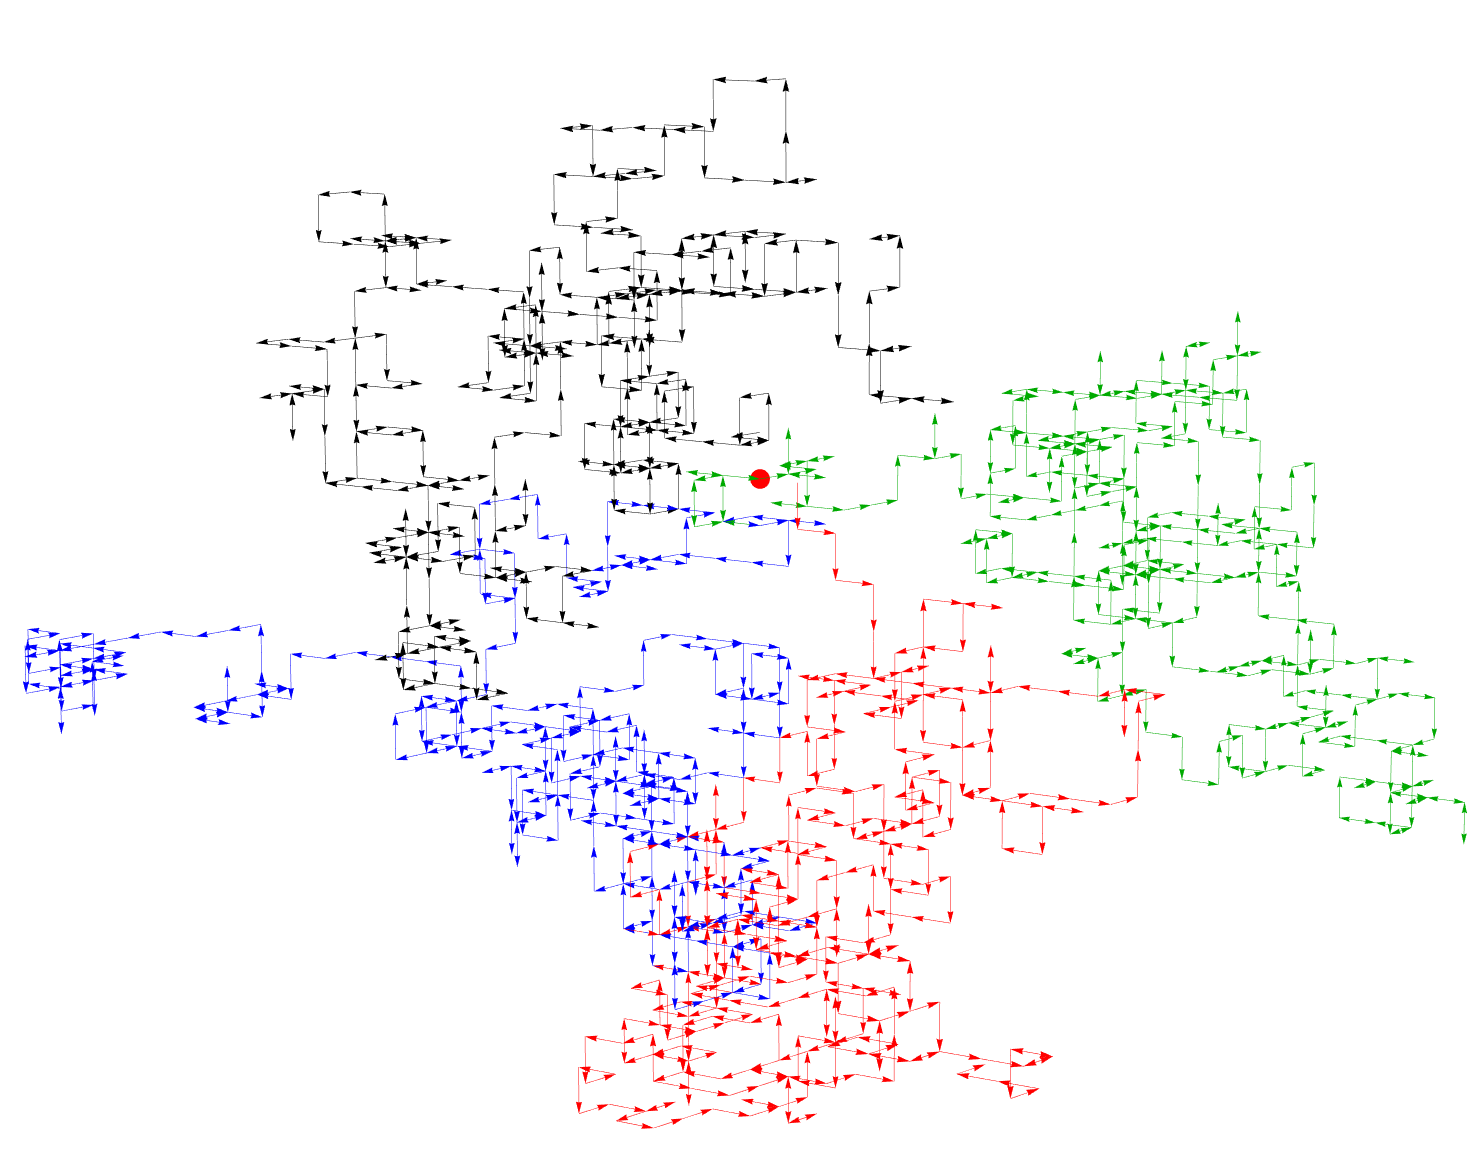
\includegraphics[width=0.8\linewidth]{Figures/quantum-walks/3d-randomwalk.png}
%     \caption{Example of three random walks on $\ZZ^3$.}
%     \label{fig:intro:3DQWs}
% \end{figure}
% \begin{wrapfigure}{r}{10cm}
%     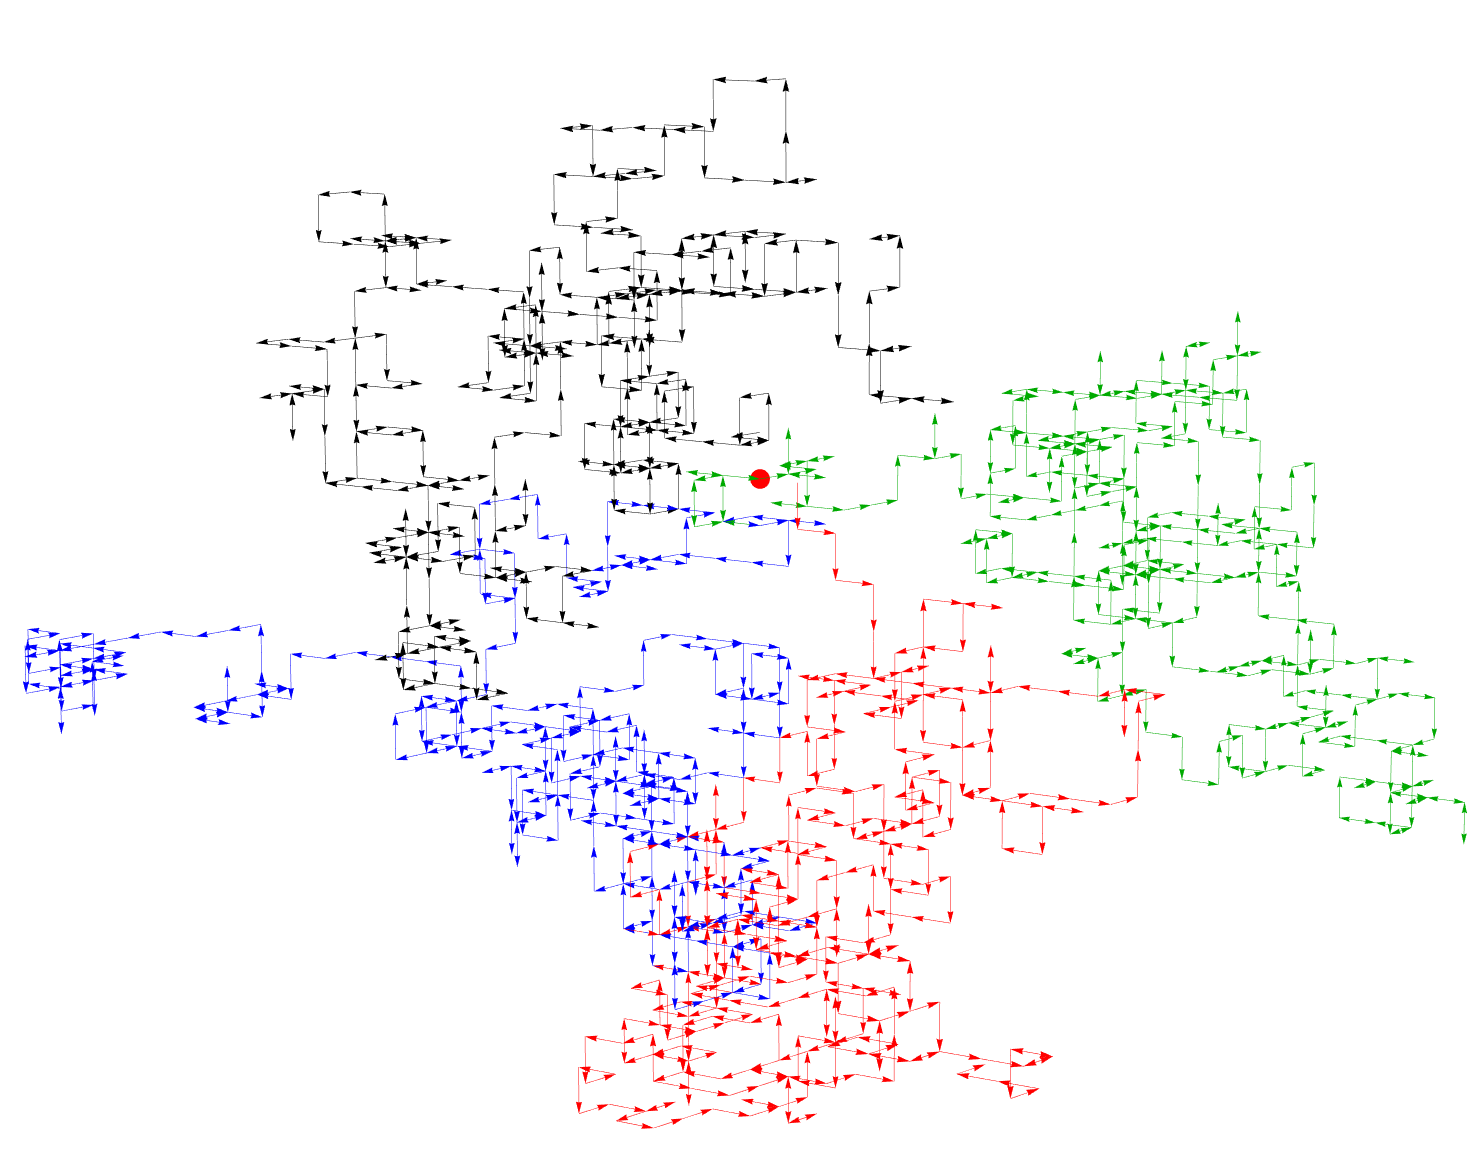
\includegraphics[width=\linewidth]{Figures/quantum-walks/3d-randomwalk.png}
%     \caption{Example of three random walks on $\ZZ^3$.}
% \end{wrapfigure}
% conversionRules = {1 -> {1, 0}, 2 -> {0, 1}, 3 -> {-1, 0}, 
%    4 -> {0, -1}};
% conversionRules3D = {1 -> {1, 0, 0}, 2 -> {0, 1, 0}, 3 -> {0, 0, 1}, 
%    4 -> {0, 0, -1}, 5 -> {0, -1, 0}, 6 -> {-1, 0, 0}};
% makeSteps[num_] := RandomInteger[{1, 4}, num] /. conversionRules;
% makeSteps3D[num_] := RandomInteger[{1, 6}, num] /. conversionRules3D;
% Graphics3D[{
%   {Red, PointSize@0.01, Point@{0, 0, 0}},
%   {Black, Arrowheads@0.005, 
%    Arrow /@ Most@Transpose@{#, RotateLeft@#} &@
%     Accumulate@makeSteps3D@400},
%   {Red, Arrowheads@0.005, 
%    Arrow /@ Most@Transpose@{#, RotateLeft@#} &@
%     Accumulate@makeSteps3D@400},
%   {Blue, Arrowheads@0.005, 
%    Arrow /@ Most@Transpose@{#, RotateLeft@#} &@
%     Accumulate@makeSteps3D@400},
%   {Darker@Green, Arrowheads@0.005, 
%    Arrow /@ Most@Transpose@{#, RotateLeft@#} &@
%     Accumulate@makeSteps3D@400}
%   },
%  (*PlotRange\[Rule]ConstantArray[{-25,25},3],Axes\[Rule]True*)
%  
%  PlotRange -> All, Boxed -> False
%  ]


% \tmpHeading{They are time-homogeneous MCs}
% The fact that the transition probability does not depend neither on the time $t$ nor on the previous history of the walker, but rather it depends exclusively on the current position, is a crucial properties of random walks, that characterises them as \textit{time-homogeneous Markov chains},
% \footnote{A \textit{Markov chain}, or \textit{Markov process}, is a generic type of stochastic process in which the probability of each event only depends on the state of the system at the previous time, rather than on the entire history of the system. Random walks are a notable example of Markov process.}
% which is a more general class of memoryless stochastic processes.

% \tmpHeading{Transition matrix}
% We can collect the set transition probabilities into a matrix $M$. This matrix will then be a \textit{bistochastic matrix}, that is a matrix satisfying $\sum_i M_{ij}=\sum_j M_{ij}=1$. If we collect the set of transition probabilities of going from $i$ to $j$ in the $i$-th column of $M$, we can then write compactly the evolution of a walk in linear algebraic notation as
% \begin{equation}
%     P_{k+1} = M P_k = M^k P_0,
% \end{equation}
% where $P_k$ is the vector of probabilities at the set $k$ ($(P_k)_i$ is the probability of finding the walker at the position $i$ at the $k$-th step).


\tmpHeading{Quantum walks}
\acp{QW} are models of quantum dynamics which share many similarities with classical random walks, and are often understood as their quantum counterparts~\cite{aharonov2000quantum,kempe2003quantum,venegasandraca2012quantum,portugal2013quantum}.
We will consider here exclusively \emph{discrete-time} \acp{QW}, which bear the more direct analogy with classical random walks. In the rest of this thesis, we will therefore always refer to this type of model when talking about ``QWs''.
In its simplest form, a \ac{QW} involves a high-dimensional system, usually referred to as \emph{walker}, endowed with an inner $2$-dimensional degree of freedom, referred to in this context as the \emph{coin}, in analogy with the classical case.
Like classical random walks, QWs are in general definable on graphs~\cite{aharonov2000quantum}, but we will limit ourselves to consider QWs \emph{on a line}, that is, QWs in which the walker can only move in one of two direction~\cite{ambainis2001onedimensional}.
A single \textit{step} of such a discrete-time \ac{QW} consists of a unitary evolution applied to the current state of the \ac{QW}. The time is therefore \emph{discrete} in the sense that there is no real notion of ``time'' as a continuous parameter. Rather, the state changes by discrete amounts at each step, just as its classical counterpart does.

% \tmpHeading{Discrete and continuous QWs}
% A first important distinction is between \textit{discrete} and \textit{continuous} \acp{QW}.
% Discrete-time QWs are systems comprised of a low-dimensional degree of freedom, usually referred to as the \textit{coin}, coupled with a high-dimensional one named the \textit{walker}.
% In this model, the time is discrete in the sense that the state evolves in discrete \textit{jumps}, rather than evolving continuously in time.
% A different model is the so-called \ac{CTQW}. Here, the dynamics is instead governed by a standard Schr\"odinger equation, and the process is therefore defined via some Hamiltonian. In a \ac{CTQW} there is no place for the notion of a \textit{coin} degree of freedom, which makes the structure of these kinds of model rather different, at least on the surface, from their discrete counterparts\highlight{(maybe mention equivalence between discrete and continuous models)}.

\tmpHeading{QWs for quantum algorithms?}
In contrast with the classical case, QWs evolve \textit{coherently}, bringing interference effects into the picture, which allows for features not found in the standard random walk model.
\acp{QW} have also been proven to be useful to develop quantum algorithms, and it was recently proved that \acp{QW} are universal for quantum compuation~\cite{childs2009universal,childs2003exponential,lovett2010universal,lovett2018quantum,underwood2010universal}.
Reviews of QW-based quantum search algorithms~\cite{ambainis2011search,ambainis2008quantum,ambainis2010developments,kempe2003quantum,kendon2006random,santha2008quantum,venegasandraca2012quantum,venegasandraca2008quantum}.
\highlight{(better literature review)}


\tmpHeading{Mathematical formalism}
The state of a QW is, for our purposes, described by a state living in a Hilbert space $\calH\equiv\calH_C\otimes\calH_W$, with $\calH_C$ a two-dimensional \emph{coin space}, and $\calH_W$ an high-dimensional space accommodating the possible states of the walker.
A generic state is thus written as
\begin{equation}
    \ket\Psi = \sum_j \sum_{s\in\{0,1\}} c_{j,s} \ket{s, j},
\end{equation}
for some coefficients $c_{j,s}\in\CC$, where $j$ spans the possible values of the walker.
The evolution of \acp{QW} is a two-step process.
First, a unitary operation is applied locally to the coin.
Then, a controlled-shift operation is applied to the walker, changing its state conditionally to that of the coin.
Formally, we write a single \textit{step operator} as $\calW=\calS\calC$, where $\calS,\calC\in\Lin(\calH)$ are linear operators on $\calH$ such that $\calC\equiv\calC\otimes I_W$.
and
\begin{equation}
    \calS = \PP_0\otimes \EE_+ + \PP_1\otimes \EE_-,
    \label{eq:qws_shitty_definition_cshift}
\end{equation}
where $\PP_k\equiv\ketbra k$ and $\EE_\pm$ are operators moving the walker in one direction or the other:
\begin{equation}
    \EE_+\equiv \sum_k \ketbra{k+1}{k},
    \qquad
    \EE_-\equiv\sum_k\ketbra{k}{k+1}.
\end{equation}
The choice of coin operation $\calC$ is what defines a particular \ac{QW}.
A standard choice is to use a \textit{Hadamard coin}, that is, $\calC=H$ where $H$ is the Hadamard matrix, defined via its action on the computational basis as
$H\ket0=\ket+$ and $H\ket1=\ket-$, where $\ket\pm\equiv\frac{1}{\sqrt2}(\ket0\pm\ket1)$.

\begin{example}[label=ex:hadamard_walk]
As an example, consider what happens with an initial state $\ket{\Psi_0}\equiv\ket{\uparrow,0}$, writing for ease of notation write the coin states as $\uparrow,\downarrow$ instead of $0$ and $1$.
The first coin operation sends this to $\ket{+,0}\equiv\frac{1}{\sqrt2}(\ket0+\ket1)$, after which the shift $\calS$ gives
\begin{equation}
    \ket{\Psi_1} \equiv 
    \calS\calC\ket{\Psi_0} =
    \calS\ket{+,0} =
    \frac{1}{\sqrt2} \left( \ket{\uparrow,+1} + \ket{\downarrow, -1} \right).
\end{equation}
The next step then sends this into
\begin{equation}
    \ket{\Psi_2} \equiv
    \frac12\left[
        \ket{\uparrow,+2} +
        (\ket{\downarrow}
        + \ket{\uparrow})\otimes \ket{0}
        - \ket{\downarrow, -2}
    \right],
\end{equation}
and then at the third step,
\begin{equation}
    \ket{\Psi_3} \equiv
    \frac{1}{2\sqrt2}\left[
        \ket{\uparrow,+3} +
        (\ket{\downarrow} + 2\ket{\uparrow})\otimes \ket{+1}
        - \ket{\uparrow,-1}
        + \ket{\downarrow,-3}
    \right].
\end{equation}
The calculation proceeds similarly for larger numbers of steps.
Note how the walker proceeds asymmetrically, even though the direct classical analogue of an Hadamard walk would be a random walk with equal probabilities of going left or right at every step.
The reason for this is in the interference effects, and the fact that the Hadamard treats $\ket\uparrow$ and $\ket\downarrow$ asymmetrically.
See~\cref{fig:hadamardwalk_Nsteps} for a simulation of the Hadamard walk with $20$ and $40$ steps, which shows clearly the asymmetry present in the output states.
\end{example}

\tmpHeading{A more efficient formalism for QWs}
One feature that emerges clearly from the above example is that, at each step, some of the possible walker's position are never occupied. More precisely, if we start with the walker at a single fixed position, say the position $\ket0$, then at odd-numbered steps only even positions will have nonzero probability amplitudes.
This symmetry can be exploited to make simulations more efficient, as well as simplify the derived expression removing modes that we know are never going to be occupied.
We will then in the following use a variation of~\cref{eq:qws_shitty_definition_cshift} in which instead of having the walker move either left or right, we have the walker either stay still or moving in one direction (say, right):
\begin{equation}
    \calS = \PP_0\otimes I + \PP_1\otimes \EE_+
    =\ketbra0\otimes I +\ketbra1\otimes\sum_k\ketbra{k+1}{k}.
\end{equation}
This notation, while somewhat nonstandard, has proven useful in some works~\cite{hoyer2009faster,montero2013unidirectional,montero2015quantum}, and will be used in~\cref{sec:intro:QWs} to obtain most of our analytical results.

\tmpHeading{The type of QWs we will consider}
We will allow the coin operation to change from step to step, while remaining site-independent~\cite{ribeiro2004aperiodic,wjcik2004quasiperiodic,bauls2006quantum}.
We demonstrate the effectiveness of this framework for the state engineering of $d$-dimensional systems and provide a set of efficiently verifiable necessary and sufficient conditions for a given state to be the output of a \ac{QW} evolution.

\begin{figure}[tb]
    \centering
    \subfloat[$20$ steps]{{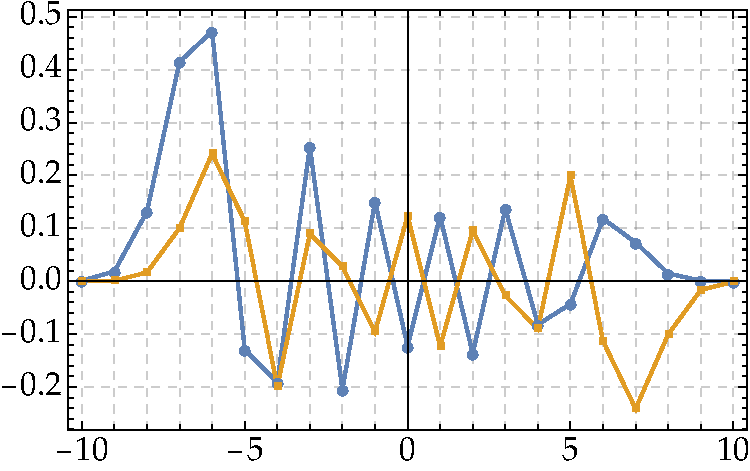
\includegraphics[width=.4\linewidth]{QW20steps_initstateUp} }}%
    \qquad
    \subfloat[$40$ steps]{{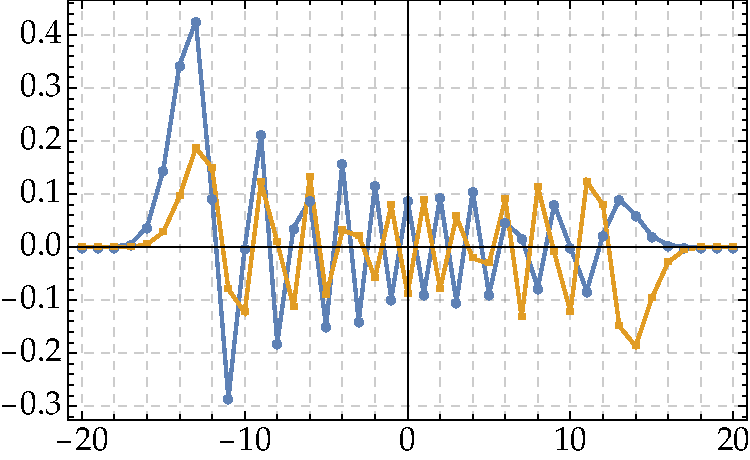
\includegraphics[width=.4\linewidth]{QW40steps_initstateUp} }}%
    % 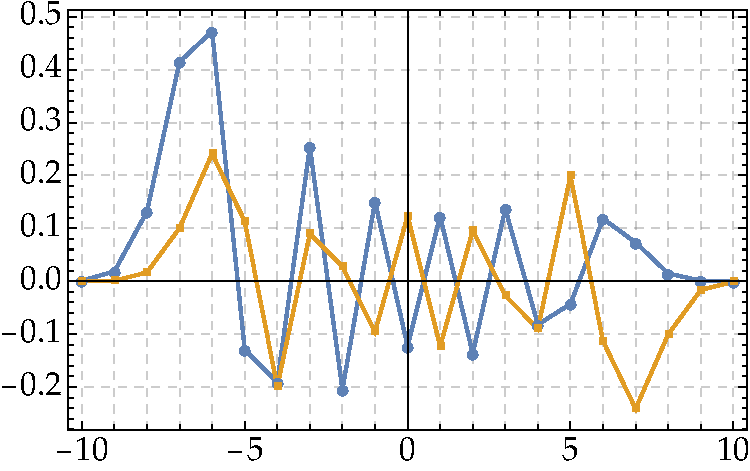
\includegraphics[width=.5\linewidth]{QW20steps_initstateUp}
    \caption{
        Output amplitudes of $20$ steps of Hadamard walk, with initial state $\ket{\Psi_0}\equiv\ket{\uparrow,0}$.
        Blue (circles) and orange (squares) points are the output amplitudes corresponding to the coin state $\ket\uparrow$ and $\ket\downarrow$, respectively.
    }
    \label{fig:hadamardwalk_Nsteps}
\end{figure}
% reindexForQW[amps_] := Transpose[
%    {{#[[1]], #[[2, 1]]}, {#[[1]], #[[2, 2]]}} & /@ 
%       Thread@{Range@Length@# - 1/2 - Length@#/2, #} &@amps
%    ];
% outAmps = 
%   QWEvolve[{1., 0}, ConstantArray[{\[Pi]/4, \[Pi]/2, \[Pi]/2}, 20], 
%     "SimulationMethod" -> "StepByStep"] // Partition[#, 2] &;
% fig = ListPlot[reindexForQW@outAmps, Joined -> True, 
%   PlotMarkers -> Automatic, Frame -> True, 
%   GridLines -> {Range[-20, 20], Range[-1, 1, 0.1]},
%   GridLinesStyle -> Directive[Opacity@.4, Gray, Dashed],
%   FrameStyle -> 
%    Directive[Black, FontFamily -> "TeX Gyre Pagella Math", 
%     FontSize -> 16]
%   ]





%! TEX program = xelatex

\chapter{Quantum Gate Learning}
\label{Section:GateLearning}

Synthesising target quantum operations is pivotal is a number of contexts in quantum information science, for example in quantum simulation~\cite{feynman1982simulating,lloyd1996universal}, quantum computation~\cite{feynman1982simulating,deutsch1985quantum,gottesman1998theory,nielsen2002quantum,ladd2010quantum}.
In particular, unitary gates play a key role in the majority of schemes for quantum computation and quantum algorithms, and more generally are a fundamental component of most quantum information protocols.

Implementing a given target unitary gate can however often be a daunting task. Different techiniques can be used to achieve this, depending on the particular experimental context and constraints.
For example, in a photonics context, one often has access to a toolbox of elementary components, such as beamsplitters and phaseshifters, which are used to build up more complex operations.
In this context, to built a complex operation $U$, one is tasked with finding a suitable combination of such elementary (generally unitary) operations $G_i$ such that $U=\prod_i G_i$. Given a fixed set of \textit{elementary gates} $\{G_i\}_i$, finding a suitable combination of these gates that results in the target operation $U$ is highly nontrivial, and is a task often referred to as the \textit{gate compilation} or \textit{gate synthesis} problem~\cite{mottonen2004quantum,nielsen2006quantum,loke2014optqc,loke2016optqc,nakajima2009synthesis,maslov2017basic,swaddle2017generating}. \highlight{(add more citations)}
\highlight{are there other experimental contexts in which it is common to have such \textit{black boxes} that are composed together?}
Solving gate compilation problems is especially important in the light of the recent significant experimental advances in the construction of experimental quantum devices, especially superconducting~\cite{devoret2013superconducting} and ion trap~\cite{blatt2008entangled,debnath2016demonstration} architectures.

A completely different type of problem is the one faced when, instead of a discrete set of gates, one is able to tune continuous parameters of an underlying dynamics.
In other words, it can be the case that the experimenter has access to some parameters $\bs\lambda$ of the system \textit{Hamiltonian} $H_{\bs\lambda}$, and wants to find the values of $\bs\lambda$ to achieve some target dynamics.
One might for example be interested in driving a fixed input to a fixed target output, or in obtaining a full effective evolution via tuning the dynamics.
In this kind of scenario, it is also common to allow for \textit{time-dependent} dynamics. This makes it much easier, in general, to achieve different types of evolutions, but at the same times makes the resulting optimisation problem that much harder, as one then has to look for an optimal \textit{function} $t\mapsto\bs\lambda(t)$, rather than just an optimal value $\bs\lambda\in\mathbb R^n$.
This types of problems are usually referred to as \textit{quantum (optimal) control} problems.
\highlight{quantum control refs}



\begin{itemize}
    \item \textbf{\textit{You can also mix these types of problems together, and/or add ancillary resources.}}
    \item The third situation is ours: we want to tune the dynamics to getter better black boxes.
    \item What's the advantages of doing it our way?
\end{itemize}

We are \cite{innocenti2018supervised}.

Open problems and solutions, literature.

\section{Standard techniques for gate engineering, previous work}
\highlight{I'm not actually sure we want this section}

\section{Time-independent dynamics for target gates}

Here, we explore a different approach to devise target unitary evolutions. More specifically, we ask the following question: is there a way to implement a given target gate \textit{without} decomposing it as a sequence of simpler gates, \textit{and} without using a time-dependent dynamics, \textit{and} without the aid of additional ancillary resources?
In other words, given a target operation $\calU$, and a set of possible candidate Hamiltonians $\calH[\bullet]\equiv \{\calH_{\bs\lambda}\}_{\bs\lambda}\subseteq\on{Herm}$\footnote{Here, $\on{Herm}\equiv\on{Herm}(N)$ is the set of Hermitian $N\times N$ matrices with complex entries, for some integer $N\ge2$. The dimension $N$ will be taken to be understood from the context.},
can we find a \textit{time-independent} Hamiltonian $\calH\in\calH[\bullet]$ such that, at some time $t$, we have $\calU = e^{-it \calH}$?
\footnote{Throughout this work, we will only consider the cases of operations and Hamiltonians acting on \textit{finite-dimensional} systems (generally sets of qubits).}
Note that if no restriction is imposed on $\calH[\bullet]$, then the problem is always trivially solvable. Indeed, writing $\calU$ in its eigendecomposition as
$\calU=\sum_k e^{i\varphi_k}\PP_k$ for some set of orthogonal projectors $\PP_j\PP_k=\delta_{jk}\PP_j$ with $\sum_k\PP_k=I_N$ and phases $\varphi_k\in\RR$, then any $\calH$ of the form
$\calH = -\sum_k \varphi_k\mathbb P_k$ satisfies $e^{-i\calH}=\cal U$.
\highlight{Do we want to prove this linear algebra stuff at some point?}
The interesting cases, both from a theoretical and practical perspective, are therefore when $\calH[\bullet]$ is constrained to have some specific structure.
Here, we will consider the case of $\calH[\bullet]$ being a set of Hamiltonians parametrised by a number of continuous parameters (in other words, it's taken to be a parametrised surface in $\on{Herm}(N)$).
We will therefore always assume that there is a continuous mapping $\RR^\ell\ni\bs\lambda\mapsto\calH(\bs\lambda)\in\on{Herm}$ such that $\calH[\bullet]=\calH(I)$ for some $I\subseteq\RR^\ell$ (which will be usually taken to equal $\RR^\ell$ for simplicity).

We can also consider the time $t$ as part of the definition of $\calH$, which amounts to a rescaling of the energy levels. We can therefore also assume $t=1$ in the following. Finally, to ease the calculations, we will consider the equivalent problem of finding $\calH$ such that $\calU=e^{i\cal H}$ (with the plus sign), as the solutions to one can be seamlessly translated into solutions to the other problem.

For concreteness, let us analyse what happens when we try to find Hamiltonian generators for a few common two- and three-qubit gates, namely the CNOT and the Toffoli gate.
\highlight{Ensure no other gates are added in the examples}
\begin{example}[label=ex:eigendecomposition_cnot]
Assume that the target operation is $\CNOT$: the two-qubit unitary gate which flips the second qubit conditionally to the value of the first one.
In matrix notation, this reads
\begin{equation}
    \on{CNOT} \equiv\begin{pmatrix}1&0&0&0 \\ 0&1&0&0 \\ 0&0&0&1\\0&0&1&0\end{pmatrix} =
    \PP_0\otimes I_2 + \PP_1\otimes X,
\end{equation}
where $\PP_k\equiv\ketbra k$ and $X$ is the Pauli $X$ gate.
The eigendecomposition of this matrix is
\begin{equation}
    \on{CNOT} =
    \ketbra{0,0} + \ketbra{0,1} + \ketbra{1,+} - \ketbra{1,-}.
    \label{eq:cnot_eigendecomposition}
\end{equation}
A more expressive way to write~\cref{eq:cnot_eigendecomposition} is by introducing the projectors $X^\pm\equiv(1\pm X)/2$, and the similarly defined $Y^\pm$ and $Z^\pm$ (here, $X,Y,Z$ denote the one-qubit Pauli matrices).
\Cref{eq:cnot_eigendecomposition} is then equivalently written as
\begin{equation}
    \on{CNOT} =
    Z^+_1 Z^+_2 + Z^+_1 Z^-_2
    + Z^-_1 X^+_2
    - Z^-_1 X^-_2
    = Z_1^+ + Z_1^- X_2^+ - Z_1^- X_2^-.
    \label{eq:cnot_eigdecomp_with_paulis}
\end{equation}
The eigenvalues are therefore $\lambda_{1,2,3}=1$ and $\lambda_4=-1$.
Can this gate be obtained via a two-qubit time-independent Hamiltonian $\calH$?
Consider for the purpose a general parametrisation of the possible two-qubit Hamiltonians, which we can write using the set of Pauli matrices on the two qubits as operatorial basis:
\begin{equation}
    \calH({\bs\lambda}) =
    \sum_{j,k=0}^4 \lambda_{j,k} \sigma^j_1\sigma^k_2.
\end{equation}
Given the decomposition of~\cref{eq:cnot_eigdecomp_with_paulis}, it is natural to use as an Ansatz for $\calH(\bs\lambda)$ an expression bearing the same eigenstructure as the CNOT. Let us therefore write
\begin{equation}
    \calH(\bs\lambda) = \lambda_1 Z_1^+ + \lambda_2 Z_1^- X_2^+ + \lambda_3 Z_1^- X_2^-.
\end{equation}
Finding $\bs\lambda\equiv(\lambda_1,\lambda_2,\lambda_3)$ such that $e^{i\calH}=\CNOT$ is then quite easy: just use $\lambda_1=\lambda_2=0$ and $\lambda_3=2\pi$. Indeed, as it is easy to check, $e^{\pi i Z_1^- X_2^-} = \CNOT$.
The natural next question is then: is this the \textbf{only} such $\calH$? It is straightforward to see that the answer is negative: for example, it is also true that $e^{\pi i n Z_1^- X_2^-}=\CNOT$ for any $n\in\ZZ$.
It is less trivial to get a complete characterisation of the solution set.
Indeed, as will be shown in~\cref{sec:solutions_matrix_equation_f(A)=B}, there is a rich set of solutions for these types of matrix equations.
\end{example}

\begin{example}[label={ex:eigendecomposition_Toffoli}]
Consider now the \textbf{Toffoli gate}, which is a three-qubit gate which flips the third qubit conditionally to the first two qubits being in the $\ket1$ state.\highlight{Ensure Toffoli was defined before, or add relevant references here.}
More explicitly, this means
\begin{equation}
    \Toff =
    \PP_0\otimes I_4 + \PP_1\otimes\CNOT
    \equiv
    \begin{pmatrix}
        I_4 & \mathbb{0}_4 \\
        \mathbb 0_4 & \CNOT
    \end{pmatrix}.
    % \begin{pmatrix}
    %     1&0&0&0&0&0&0&0 \\
    %     0&1&0&0&0&0&0&0 \\
    %     0&0&1&0&0&0&0&0 \\
    %     0&0&0&1&0&0&0&0 \\
    %     0&0&0&0&1&0&0&0 \\
    %     0&0&0&0&0&1&0&0 \\
    %     0&0&0&0&0&0&0&1 \\
    %     0&0&0&0&0&0&1&0
    % \end{pmatrix}
\end{equation}
In terms of projectors onto eigenvalues of (products of) Pauli matrices, we have
\begin{equation}
    \Toff = Z_1^+ + Z_1^- Z_2^+ + Z_1^- Z_2^- X_3^+ - Z_1^- Z_2^- X_3^-.
\end{equation}
The eigenvalues of $\Toff$ are thus readily seen to be $+1$ with multiplicity $7$, and $-1$ with multiplicity $1$.
A possible $\calH$ such that $e^{i\cal H}=\Toff$ is then $\calH=\pi Z_1^- Z_2^- X_3^-$.
Note how expanding this Hamiltonian we get
\begin{equation}
    \calH = \frac{\pi}{8}\left[
        I - (Z_1 - Z_2 - X_3)
        + (Z_1 Z_2 + Z_1 X_3 + Z_2 X_3)
        - Z_1 Z_2 X_3
    \right],
\end{equation}
which contains three-qubit interaction terms (the $Z_1 Z_2 X_3$ factor). While this is to be expected , as the Toffoli is a non-trivial three-qubit gate, these kinds of terms make practically implementing these Hamiltonians significantly harder.
Indeed, natural interactions, and in particular interactions that can be easily implemented in experiments, generally \highlight{can we promote this to \textbf{always}?} involve only one- and two-qubit interaction terms.
It is then natural to wonder about whether this is a \textbf{necessary} feature of time-independent generators of the Toffoli gates.
As will be shown in the following sections, the answer is in fact that yes, it is possible to find time-independent Hamiltonians that generate a Toffoli gate \textbf{and} only use up to two-qubit interactions.
\end{example}

As shown in~\cref{ex:eigendecomposition_cnot,ex:eigendecomposition_Toffoli}, looking for Hermitian generators of few-qubit gates is not a fairly straightforward task. There are, however, two notable issues with the type of analysis conducted so far:
\begin{enumerate}
    \item It lacks in generality: while finding specific generators essentially amounts to computing the eigendecomposition of the target $\calU$, and then the logarithm of the eigenvalues, this says nothing about whether such procedure provides the most general kind of Hamiltonian generator for the given gate. In other words, can \textit{all} generators $\calH$ be obtained this way?
    \item We have no control over the kind of generators that we obtain with this procedure. For example, in~\cref{ex:eigendecomposition_cnot} we obtained generators containing two-qubit interactions of the form $Z_1 X_2$. Does this mean that this type of interaction term is \textit{necessary} to generate a CNOT? Or is there instead some Hamiltonian that can still generate the CNOT without using such terms?
    Similar questions arise in~\cref{ex:eigendecomposition_Toffoli}.
\end{enumerate}
To address these issues, we will study the underlying mathematical problem in more depth. As it turns out, we can divide such analysis in two parts. In~\cref{sec:solutions_matrix_equation_f(A)=B}, we show how to find general solutions to inverse matrix equations of the form $f(A)=B$. Then, in~\cref{sec:constraints_on_interaction_pars}, we present a way to bring additional constraints on the interaction terms into the discussion.
\highlight{to review this part probably}

\section{Solutions of the matrix equation \texorpdfstring{$f(A)=B$}{f(A)=B}}
\label{sec:solutions_matrix_equation_f(A)=B}
Let $A,B$ be normal matrices such that $f(A)=B$ for some function $f$ (assumed to be regular on the spectrum of $A$), with $f(A)$ defined as usual on the eigenvalues of $A$.
In this section we will provide a full characterisation of the set of solutions $A\in f^{-1}(B)$ .

Explicitly, $f(A)=B$ amounts to
\begin{equation}
    \sum_j \lambda_j^B \PP_j^B = \sum_k f(\lambda_k^A) \PP_k^A,
    \label{eq:f(A)=B_eigendecomp_proof}
\end{equation}
where $\PP_k^{A} (\PP_k^{B})$ are the projectors onto the corresponding eigenspaces of $A$ and $B$, so that
$A\PP_k^A=\lambda_k \PP_k^A$, and similarly for $B$.
Because both sides of~\cref{eq:f(A)=B_eigendecomp_proof} define the eigendecomposition of some (normal) operator, by the uniqueness of the eigendecompositions it follows that $\lambda_j^B=f(\lambda_j^A)$ and $\PP_j^B=\PP_j^A$.
What is interesting about this is that it means that the relation $f(A)=B$ puts strong constraints on the eigenstructure of $A$: the eigenspaces of $A$ must be the same as those of $B$.

Consider now the problem of finding a matrix $A$ such that $f(A)=B$, for some predetermined mapping $f$.
If $f$ is injective (at least on $f^{-1}(\sigma(B))$), then, by our above argument, it follows that $A$ is uniquely determined. Indeed, we the condition would then be
\begin{equation}
    \sum_j \lambda_j^B \PP_j = \sum_j f(\lambda_j^A) \PP_j,
\end{equation}
which can only be true for $\lambda_j^A = f^{-1}(\lambda_j^B)$.
However, because we are considering here matrices and functions defined over $\CC$, most interesting cases will correspond to \textit{non-injective} functions $f$\footnote{Indeed, the only entire, injective functions $\CC\to\CC$ are the linear mappings $z\mapsto az+b$ for some $a,b\in\CC$.}. The case $f(z)=e^z$, which is the one with which we will be mostly concerned with for the gate learning problem, is one such case of non-injective function.

When $f$ is non-injective, there can be multiple $A$ such that $f(A)=B$. There are two main reasons for this, one fairly evidence, and the other one less so.
Clearly, being $f$ not injective, for any given eigenvalue $\lambda_j^B$ there can be multiple $\lambda$ such that $f(\lambda)=\lambda_j^B$. This is indeed the only source of non-uniqueness whenever the eigenspaces of $B$ are all one-dimensional (equivalently, the projetors $\PP_k^B$ in~\cref{eq:f(A)=B_eigendecomp_proof} have all unit trace).
However, whenever there are eigenspaces of dimension greater than one, there are multiple (infinite) ways to write a corresponding projector $\PP$ as sum of unit-trace projectors. Assume for example that $\Tr\PP=d$, and let $\PP_k$ be a set of $d$ unit-trace projectors such that $\PP=\sum_{k=1}^d \PP_k$. Let $U$ be an arbitrary operator that is unitary in the range of $\PP$.
Then we have
\begin{equation}
    \PP=U^\dagger \PP U =\sum_{k=1}^d U^\dagger \PP_k U
    \equiv \sum_{k=1}^d \tildePP_k,
    \label{eq:rewriting_proj_with_rotated_projs}
\end{equation}
where we defined the ``rotated projectors'' $\tildePP_k\equiv U^\dagger \PP U$.
While this rewriting is ininfluent in~\cref{eq:rewriting_proj_with_rotated_projs}, such rotations of the degenerate eigenspaces turn out to be of great relevance when looking for solutions of $f(A)=B$.
To see this, let us consider again~\cref{eq:f(A)=B_eigendecomp_proof}, and focus on a single eigenspace $\PP_j^B$ such that $\Tr\PP_j^B=d_j>1$ (assuming $B$ has one), and write an arbitrary decomposition of $\PP_j^B$ in terms of on unit-trace projectors as $\PP_j^B=\sum_{\ell=1}^{d_j}\PP^B_{j,\ell}$.
Let $\{\lambda_{j,\ell}\}_{\ell=1}^{d_j}\subseteq f^{-1}(\lambda_j^B)$ be a subset of inverses of $\lambda_j^B$. Then, any $A$ which has $\lambda_{j,\ell}$ as eigenvalues within the eigenspace $\PP_j^B$ is a suitable solution for $f^{-1}(B)$.
In other words, we have
\begin{equation}
    A \equiv \sum_j \sum_{\ell=1}^{d_j} \lambda_{j,\ell} \PP_{j,\ell}\in f^{-1}(B),
    \quad \forall \lambda_{j,\ell}\in\CC \text{ with } f(\lambda_{j,\ell})=\lambda_j^B.
    \label{eq:general_form_f-1B}
\end{equation}
Note how this means that $f^{-1}(B)$ \textit{can break the degeneracies in $B$} thanks for the non-injectivity of $f$.

Let us give now a few concrete examples of the freedom allowed by the degeneracies.

\begin{example}[label={ex:solutions_f(A)=I2}]
Consider the two-dimensional identity matrix $I_2$, and an arbitrary complex function $f$ defined on the complex unit. \textbf{What is then the set of matrices $A$ such that $f(A)=I_2$?}
Note that $I_2=P+Q$ for any pair of orthogonal projectors $P,Q$, and $\lambda P + \mu Q\in f^{-1}(I_2)$ for any $\lambda,\mu\in f^{-1}(1)$.
This can be equivalently stated saying that, for any pair of orthonormal states $\ket u$ and $\ket v$, we have
$\lambda \ketbra u + \mu \ketbra v\in f^{-1}(I_2)$.
Going further, we parametrise the set of all such vectors writing (we can define the vectors up to an overall phase, as we are only interested in the corresponding projectors):
\begin{equation}
    \begin{cases}
    \ket u =\cos\alpha\ket 0+e^{i\theta}\sin\alpha \ket 1, \\
    \ket v =-e^{-i\theta}\sin\alpha\ket 0 + \cos\alpha\ket 1.
\end{cases}
\end{equation}
This provides us with a parametrisation for the set of solutions $f^{-1}(B)$:
\begin{equation}
\begin{aligned}
    A = &\lambda\left(\cos^2(\alpha) \PP_0 + \sin^2(\alpha) \PP_1 + \sin(2\alpha)\Re[e^{i\theta}\ketbra{1}{0}]\right) \\
    +&\mu\left(
        \sin^2(\alpha) \PP_0 + \cos^2(\alpha) \PP_1 - \sin(2\alpha)\Re[e^{i\theta}\ketbra{1}{0}]
    \right),
\end{aligned}
\end{equation}
or in matrix form,
\begin{equation}
    A = \begin{pmatrix}
        \lambda \cos^2(\alpha)+\mu\sin^2(\alpha) &
        \frac12 e^{-i\theta} \sin(2\alpha) (\lambda-\mu) \\ 
        \frac12 e^{i\theta} \sin(2\alpha) (\lambda-\mu) &
        \lambda \sin^2(\alpha)+\mu\cos^2(\alpha)
    \end{pmatrix}.
    \label{eq:explicit_inverse_f(A)_matrix_form}
\end{equation}
We conclude that any such $A$ is such that $f(A)=I_2$, as long as $f(\lambda)=f(\mu)=1$, and that this form covers the set of all possible normal matrices satisfying this equation.
Whenever $\lambda=\mu$,~\cref{eq:explicit_inverse_f(A)_matrix_form} reduces to $A=\lambda I_2$, which is the trivial solution. When $\lambda\neq\mu$, however, it is less obvious that the corresponding matrix in~\cref{eq:explicit_inverse_f(A)_matrix_form} satisfies $f(A)=I_2$.
\end{example}

\begin{example}[label={ex:solutions_f(A)=I_3}]
\highlight{To decide where to put this crap.}

Consider how to split the eigenspace of the three-dimensional identity $I_3$.
This essentially amounts to the problem of parametrising a set of three orthonormal complex vectors. For the purpose, let us write them as
\begin{equation}
\begin{cases}
    \ket{u_1} = \cos(\alpha)\ket0
    + e^{i\theta}\sin(\alpha)\cos(\beta)\ket1
    + e^{i\varphi}\sin(\alpha)\sin(\beta)\ket2, \\
    \ket{u_2} = \cos(\alpha)\ket0
    + e^{i\theta}\sin(\alpha)\cos(\beta)\ket1
    + e^{i\varphi}\sin(\alpha)\sin(\beta)\ket2, \\
\end{cases}
\end{equation}
\highlight{Actually, there might not be a general nice way to parametrise such sets of vectors!}
\end{example}

\begin{example}[label={ex:solutions_e^A=I2}]
Picking up from~\cref{ex:solutions_f(A)=I2}, let us analyse the solutions to $f(A)=I_2$ when $f(z)=e^z$.
Then $f^{-1}(1)=2\pi i\ZZ$, and the set of solutions becomes
\begin{equation}
    A_{\alpha,\theta;n,m} = 2\pi i
    \begin{pmatrix}
        n \cos^2(\alpha)+m\sin^2(\alpha) &
        \frac12 e^{-i\theta} \sin(2\alpha) (n-m) \\ 
        \frac12 e^{i\theta} \sin(2\alpha) (n-m) &
        n \sin^2(\alpha)+m\cos^2(\alpha)
    \end{pmatrix},
\end{equation}
for all $n,m\in\ZZ$ and $\alpha,\theta\in\RR$.
\end{example}

\begin{example}[label={ex:cnot_generator_decomposition}]
We gave in~\cref{ex:eigendecomposition_cnot} a possible Hamiltonian generator for the CNOT gate.
Here, strong on the general characterisation of matrix inverses given in~\cref{eq:general_form_f-1B}, we work out a more general expression for the set of Hamiltonians $\calH$ such that $e^{i\calH}=\CNOT$.
Specialising~\cref{eq:general_form_f-1B} to the specific eigenstructure of $\CNOT$ (which we worked out in~\cref{ex:eigendecomposition_cnot}), we see that a generic (normal) generator for $\CNOT$ has the form
\begin{equation}
    \sum_{j=1}^3 \lambda_j \tildePP_j + \mu\PP_4,
\end{equation}
where
$\PP_4\equiv\ketbra 4\equiv\ketbra{1,-}$, the projectors 
$\{\tildePP_j\}_{j=1}^3$ define an arbitrary splitting of the degenerate eigenspace $\ker[(\CNOT-I_4)]$ into orthonormal vectors, and $\lambda_j,\mu\in\CC$ are such that $e^{i\lambda_j}=1$ and $e^{i\mu}=-1$.
These last conditions identify $\lambda_j\in2\pi\ZZ$ and $\mu\in\pi + 2\pi\ZZ$.
% \begin{equation}
%     \lambda_{j,\ell} = 2\pi n_{j,\ell},
%     \quad
%     \mu_\ell = \pi + 2\pi m_\ell,
%     \quad
%     n_{j,\ell},m_\ell\in\ZZ.
% \end{equation}
A generic generator for the CNOT can thus be written as
\begin{equation}
    \calH =
    2\pi\left[
    \sum_{j=1}^3 n_j \tildePP_j +
    \frac{1}{2} m\PP_4
    \right].
\end{equation}
It is worth stressing how the set of viable generators $\calH$ has both a discrete and a continuous degree of freedom.
\end{example}

In the rest of the thesis, we will focus on the case $f(A)\equiv e^{iA}$, which is case of relevance to find Hamiltonians generating target unitaries.

\section{Adding physical practical constraints}
\label{sec:constraints_on_interaction_pars}

In~\cref{sec:solutions_matrix_equation_f(A)=B} we described how to write the full set of solution for a matrix equation of the form $f(A)=B$.
In this section we will show how introducing further constraints on the type of interaction terms allowed in the final generator reveals a particularly daunting task.

To restrict the type of interaction terms allowed in the final generator, means to fix some set $\calP$ comprised of orthogonal Hermitian operators $\sigma_i$, and ask for a generator $\calH\in f^{-1}(\calU)$ such that $\calH$ is in the span of $\{\sigma_i\}_i$:
\begin{equation}
    \calH \in f^{-1}(\calU) \cap \on{Span}\calP.
\end{equation}
In the following, we will focus on the case  $f(A)\equiv e^{iA}$. \highlight{probably need to specify what is $f$ here}
A typical (but not necessary) choice for the $\sigma_i$ is the set of one- and two-qubit interaction terms $\calP_{\le2}$, defined as
\begin{equation}
    \calP_{\le2} \equiv \{ I, X_i,Y_i,Z_i, X_i Y_j, X_i Z_j, Y_i Z_j : \,\,i,j=1,2,3 \}.
\end{equation}
We thus have for example $X_i,Y_j\in\calP_{\le2}$ and $X_i Z_j\in\calP_{\le2}$, but $X_i Y_j Z_k\notin\calP_{\le2}$ for $i\neq j,i\neq k$ and $j\neq k$.

Given a candidate generator $\calH\in f^{-1}(\calU)$, one would therefore need to decompose $\calH$ in a basis containing the elements of $\calP$, and impose that all terms outside of this set are vanishing.
Given a target gate with eigendecomposition
$\calU=\sum_j e^{i\varphi_j}\PP_j$ with $\Tr\PP_j=d_j$ and $\sum_j d_j=2^n$ with $n$ the number of qubits, this would entail in practice finding bases for each $\on{Range}(\PP_j)$ built out of states $\{\ket*{u_{jk}}\}_{k=1}^{d_j}\subset \mathbb{CP}^{d_j}$, and integers $n_{jk}$, such that
\begin{equation}
    \sum_j\sum_{k=1}^{d_j} (\varphi_j + 2\pi n_{jk}) \PP[\ket*{u_{jk}}]
    \in \on{Span}_{\RR}\calP.
\end{equation}

\begin{example}[label={ex:cnot_physical_constraints}]
Let $\calU=\CNOT$, and consider a set of allowed interactions containing only single-qubit terms: $\calP_1\equiv\{X_i,Y_i,Z_i\}_{i\in\{1,2\}}$.
Is there an $\calH$ containing only interactions in $\calP_1$ and such that $e^{i\calH}=\CNOT$?

From a physical point of view, the answer should obviously be that no, there cannot be any such Hamiltonian, as that would mean that an entangling two-qubit gate can be obtained without having the qubits interact in any way.
Still, it is interesting to see if we can recover this result using the formalism introduced in the previous section, as a testbed to see it in action.
Consider then the decomposition given in~\cref{ex:cnot_generator_decomposition} for the CNOT:
\begin{equation}
    \calH =
    2\pi\left[
    \sum_{j=1}^3 n_j \tildePP_j +
    \frac{1}{2} m\PP_4
    \right],
\label{eq:cnotex_general_H_expr}
\end{equation}
where
$\PP_4\equiv Z_1^- X_2^-$ and $\tildePP_1,\tildePP_2,\tildePP_3$ define an arbitrary splitting of the eigenspace generated by $\ket{0,0},\ket{0,1}$ and $\ket{1,+}$.
Let us write down explicitly the decompositions of these projectors in terms of Pauli matrices:
\begin{equation}
\begin{cases}
    \tildePP_1 &= Z_1^+ Z_2^+ \,= \frac{1}{4} (I + Z_1 + Z_2 + Z_1 Z_2), \\
    \tildePP_2 &= Z_1^+ Z_2^- \,= \frac{1}{4} (I + Z_1 - Z_2 - Z_1 Z_2), \\
    \tildePP_3 &= Z_1^- X_2^+ = \frac{1}{4} (I - Z_1 + X_2 - Z_1 X_2), \\
    \PP_4 &= Z_1^- X_2^- = \frac{1}{4} (I - Z_1 - X_2 + Z_1 X_2),
\end{cases}
\end{equation}
where we made a canonical choice for the $\tildePP_i$.
Without exploiting the freedom given by the degeneracies, it is straightforward to see that it is not possible to find values for the $n_j\in\ZZ$ such annihilate the two qubit interaction terms, due to the $1/2$ factor in~\cref{eq:cnotex_general_H_expr}.
Indeed, expanding~\cref{eq:cnotex_general_H_expr} and focusing on the two-qubit interaction terms, we get
\begin{equation}
    \calH = (...) + \frac{2\pi}{4}\left[
    (n_1 - n_2) Z_1 Z_2 +
    (n_4/2 - n_3) Z_1 X_2
    \right].
\end{equation}
Remarkably, this shows how the $Z_1 X_2$ seems to be a necessary part of a generator, as there is no choice of $n_3,n_4\in\ZZ$ such that $n_4-2 n_3=0$.
Still, this does not rule out the possibility that for some other choice of $\tildePP_j$ it is possible.
The difficulty in showing this in full generality arises from the lack of a nice general expression for a arbitrary unitary rotations in more than two dimensions \highlight{maybe make sure this is actually true. What about Jarlskogwhateverthefuckitscalled decomposition?}.
In~\cref{sec:gatelearning_solution_framework} we will provide a way to answer these questions more easily.
\end{example}

\begin{example}[label={ex:toffoli_physical_constraints}]
Let $\UToff$ denote the Toffoli gate, and consider the set of allowed interactions $\calP_{\le2}$ comprised of one- and two-qubit interaction terms (but notably \textit{not} three-qubit terms).
\textbf{\textit{Is there a generator $\HToff\in f^{-1}(\UToff)\cap\calP_{\le2}$?}}

The eigenstructure of the Toffoli gate was given in~\cref{ex:eigendecomposition_Toffoli}. Similarly to the case of the CNOT, we here have a sevenfold degenerate eigenvalues $+1$ and a nondegenerate eigenvalue $-1$.
The eigenvector of the eigenvalue $-1$ is $\ket{1,1,-}$. We can therefore write a general expression for generators of $\Toff$ in the form
\begin{equation}
    \calH=2\pi \left[
        \sum_{j=1}^7 n_j \tildePP_j
        +\frac12 m\PP_8,
    \right]
\end{equation}
where $\PP_8\equiv\ketbra{1,1,-}$ and $\sum_{j=1}^7\tildePP_j+\PP_8=I_8$.
Note how the choice $n_j=0$ gives a generator proportional to $\PP_8$, which contains the three-qubit interaction term $Z_1 Z_2 X_3$, and is therefore not contained in $\calP_{\le2}$.
A canonical choice for the $\tildePP_j$ is the following:
\begin{equation}
\begin{cases}
    \tildePP_1 &= Z_1^+ Z_2^+ Z_3^+ = (...) + \frac18 Z_1 Z_2 Z_3, \\
    % = \frac{1}{8} (I + Z_1 + Z_2 + Z_3 + Z_1 Z_2 + Z_1 Z_3 + Z_2 Z_3 + Z_1 Z_2 Z_3), \\
    \tildePP_2 &= Z_1^+ Z_2^+ Z_3^- = (...) - \frac{1}{8} Z_1 Z_2 Z_3, \\
    %\,= \frac{1}{4} (I + Z_1 - Z_2 - Z_1 Z_2), \\
    \tildePP_3 &= Z_1^+ Z_2^- Z_3^+ = (...) - \frac18 Z_1 Z_2 Z_3, \\
    \tildePP_4 &= Z_1^+ Z_2^- Z_3^- = (...) + \frac18 Z_1 Z_2 Z_3, \\
    \tildePP_5 &= Z_1^- Z_2^+ Z_3^+ = (...) - \frac18 Z_1 Z_2 Z_3, \\
    \tildePP_6 &= Z_1^- Z_2^+ Z_3^- = (...) + \frac18 Z_1 Z_2 Z_3, \\
    \tildePP_7 &= Z_1^- Z_2^- X_3^+ = (...) + \frac18 Z_1 Z_2 X_3, \\
    \PP_8 &= Z_1^- Z_2^- X_3^- = (...) - \frac18 Z_1 Z_2 X_3.
\end{cases}
\end{equation}
Similarly to what we found in~\cref{ex:cnot_physical_constraints}, we have here a three-qubit interaction term, $Z_1 Z_2 X_3$, which is proportional to $(n_7 - m/2)$, and therefore cannot be removed by any choice of the integer parameters.
% \begin{equation}
%     (n_7 - m/2) Z_1 Z_2 X_3
% \end{equation}
There is, however, a marked difference between the present case and~\cref{ex:cnot_physical_constraints}: while for the CNOT we have strong physical reasons to believe that it is impossible to obtain the gate without two-qubit interaction terms, this is not the case for the Toffoli.
Indeed, while it is in principle possible to achieve a three-qubit entangling gate without using three-qubit interaction terms, although the veracity of this claim is not obvious.
Indeed, we will show in~\cref{sec:gatelearning_solution_framework} how, by appropriately rotating the degenerate eigenspace, it \textit{is} possible to achieve such a feat.
\end{example}

\section{A solution framework}
\label{sec:gatelearning_solution_framework}
As demonstrated in~\cref{sec:constraints_on_interaction_pars}, injecting physical constraints into the problem makes it significantly harder to solve.
Nevertheless, we will show in this section how a few observations can be exploited to significantly simplify the task.

Piggybacking on the results of~\cref{sec:solutions_matrix_equation_f(A)=B}, consider the general problem of looking for generators $\calH$ such that $e^{i\calH}=\calU$ for a given unitary $\calU$.
While, as previously discussed, there are in general many possible such $\calH$, there \textit{is} one ``natural'' choice that can be considered as \textit{canonical} in this context.
Indeed, while a generic $\calH$ can break the degeneracies of $\calU$, let us denote with $\calH_{\calU}$ a \textit{canonical generator}, which is one that preserves the degeneracies of $\calU$.
Note that computing such a generator is generally a straightforward task.
% Indeed, given an eigendecomposition of $\calU$ 
% As previously discussed, it is easy to find \textit{one} possible $\calH$ satisfying this requirement. Let us denote such a ``canonical'' generator with $\calH_{\calU}$.
Any other generator $\calH$ will have to be related to $\calH_{\calU}$ through the equation $e^{i\calH}=e^{i\calH_{\calU}}=\calU$.
We will show in this section that the following two conditions must be always satisfied by any such $\calH$:
\begin{itemize}
    \item Every such $\calH$ must commute with $\calH_{\calU}$.
    % : $[\calH,\calH_{\calU}]=0$.
    \item The eigenvalues of $\calH-\calH_{\calU}$ must all be integer multiples of $2\pi$.
\end{itemize}

Indeed, assume that $\calH$ and $\calH_{\calU}$ satisfy these two conditions.
% Then, as shown in~\cref{sec:solutions_matrix_equation_f(A)=B}, 
While, in general, two Hamiltonians $\calH_1,\calH_2$ with $e^{i\calH_1}=e^{i\calH_2}=\calU$ need not commute with each other, this must be the case when one of the two is a canonical generator $\calH_{\calU}$. In other words, we must always have $[\calH,\calH_{\calU}]=0$.
This is for the same reason why, for any generator $\calH$, we must have $[\calH,\calU]=0$.
Moreover, $[\calH,\calH_{\calU}]=0$ implies that
$I=e^{i\calH}e^{-i\calH_{\calU}}=e^{i(\calH-\calH_{\calU})}$.
But for this to be true, the eigenvalues of $\calH-\calH_{\calU}$ must necessarily be integer multiples of $2\pi$, which proves the first implication.

For the other direction, let us assume that, given some $\calH_{\calU}$ such that $e^{i\calH_{\calU}}=\calU$, we have $[\calH,\calH_{\calU}]=0$ and $\on{Spec}(\calH-\calH_{\calU})\subseteq2\pi\ZZ$.
Then,
\begin{equation}
    e^{i\calH} =
    e^{i\calH} e^{-i\calH_{\calU}} e^{i\calH_{\calU}} =
    e^{i(\calH-\calH_{\calU})} \calU =
    \calU.
\end{equation}
This suggests the following plan of action to solve the general problem in the presence of constraints on the Hamiltonian generators: let $\calU$ be a target gate with canonical generator $\calH_{\calU}$. Then, to find $\calH\in f^{-1}(\calU)\cap\calP$ is equivalent to find $\calH$ satisfying the following three conditions:
\begin{subequations}
\begin{gather}
    \calH\in\calP, \label{eq:3conditions_1st}\\
    [\calH,\calU]=0 \text{ (equivalently, $[\calH,\calH_{\calU}]=0$)}, \label{eq:3conditions_2nd}\\
    \on{Spectrum}(\calH-\calH_{\calU})\subseteq2\pi\ZZ \label{eq:3conditions_3rd}
\end{gather}
\label{eq:3conditions}
\end{subequations}
% \begin{enumerate}
%     \item $\calH\in\calP$,
%     \item $[\calH,\calU]=0$ (or, equivalently, $[\calH,\calH_{\calU}]=0$),
%     \item $\on{Spectrum}(\calH-\calH_{\calU})\subseteq2\pi\ZZ.$
% \end{enumerate}
To approach a given problem, we can therefore proceed as follows:
1) write a general expression for an element in the (real) span of $\calP$: $\calH=\sum_k c_k \sigma_k$ summed over all $\sigma_k\in\calP$.
2) Impose $[\calH,\calU]=0$, this immediately cuts many of the coefficients in the general expression for $\calH$.
3) Look into the remaining set of coefficients $c_k$ for a combination that satisfies the third condition.

Note how the first two conditions are easy to impose, while the third one remains difficult. To see this more concretely let us consider a few applications of this framework.

\begin{example}[label={ex:cnot_with_conditions}]
Taking up where we left off in~\cref{ex:cnot_physical_constraints}, let us see if~\cref{eq:3conditions} can give us a conclusive way to prove the impossibility of generating a CNOT with only one-qubit interactions.
A canonical generator for the CNOT is obtained by setting $n_i=0$ and $m=1$ in~\cref{eq:cnotex_general_H_expr}, which results in
$\calH_{\CNOT}=\pi Z_1^- X_2^-$.
A general form for an $\calH$ containing one-qubit interactions is
\begin{equation}
    \calH = h_0 I +
    \sum_{\alpha=1}^3 (h_1^\alpha\sigma_1^\alpha + h_2^\alpha\sigma_2^\alpha),
\end{equation}
where $\sigma_i^1\equiv X_i, \sigma_i^2\equiv Y_i, \sigma_i^3\equiv Z_i$.
Imposing $[\calH,\CNOT]=0$ removes most of the parameters, leaving us with the simplified expression
\begin{equation}
    \calH = h_0 I_4 + h_1^3 Z_1 + h_2^1 X_2.
    \label{eq:cnot_expr_after_commutativity_condition}
\end{equation}
One easy way to see this is to note that for $\calH$ to commute with $\CNOT$, the two matrices must respect each other's eigenspaces. In particular, this means that $\calH$ must preserve the nondegenerate eigenvector of $\CNOT$, which is $\ket{1,-}$.
The only one-qubit gates that do this are $I_4, Z_1$ and $X_2$, hence we arrive to~\cref{eq:cnot_expr_after_commutativity_condition}.

The question is now reduced to that of figuring out whether there are coefficients $h_0,h_1^3,h_2^1\in\RR$ such that the spectrum of $\calH-\calH_{\CNOT}$ contains nothing but integer multiples of $2\pi$.
In matrix form,~\cref{eq:cnot_expr_after_commutativity_condition} reads
\begin{equation}
    \calH = \begin{pmatrix}
        h_0 + h_1^3 & h_2^1 & 0 & 0 \\
        h_2^1 & h_0 + h_1^3 & 0 & 0 \\
        0 & 0 & h_0 - h_1^3 & h_2^1 \\
        0 & 0 & h_2^1 & h_0 - h_1^3
    \end{pmatrix},
\end{equation}
which has the four eigenvalues $h_0\pm h_1^3 \pm h_2^1$.
At the same time,
\begin{equation}
    \calH_{\CNOT} = \frac{\pi}{2}\begin{pmatrix}
        0 & 0 & 0 & 0 \\
        0 & 0 & 0 & 0 \\
        0 & 0 & 1 & -1 \\
        0 & 0 & -1 & 1
    \end{pmatrix},
\end{equation}
which has eigenvalues $\pi,0$. The eigenvalues of $\calH-\calH_{\CNOT}$ are then
\begin{equation}
\def\id{h_0}
\def\Z1{h_1^3}
\def\X2{h_2^1}
\begin{cases}
    \id + \Z1 - \X2 &= 2\pi \nu_1, \\
    \id - \Z1 + \X2 &= 2\pi \nu_2, \\
    \id + \Z1 + \X2 &= 2\pi \nu_3, \\
    \id - \Z1 - \X2 - \pi &= 2\pi \nu_4.
\end{cases}
\end{equation}
Inverting this system, we get from the first three equations
\begin{equation}
\def\id{h_0}
\def\Z1{h_1^3}
\def\X2{h_2^1}
\begin{cases}
    \id &= \pi (\nu_1 + \nu_2), \\
    \X2 &= \pi (\nu_3 - \nu_1), \\
    \Z1 &= \pi (\nu_3 - \nu_2).
\end{cases}
\end{equation}
However, using now these with the fourth equation, we arrive to the condition
\begin{equation}
    2(\nu_1 + \nu_2 - \nu_3 - \nu_4) = 1,
\end{equation}
which is clearly unsatisfiable for integer $\nu_i\in\ZZ$.

It is worth noting that, of course, this result could have been obtained more easily from a more physical line of reasoning. Indeed, an Hamiltonian $\calH$ containing only one-qubit interactions can always be written as $\calH=h_0 I+\calH_1+\calH_2$ with $\calH_i$ containing only one-qubit terms on the $i$-th qubit. Then, $[\calH_1,\calH_2]=0$, and therefore
\begin{equation}
    e^{it\calH}=e^{it h_0}e^{it\calH_1}e^{it\calH_2}=e^{it h_0} \calU_1\otimes\calU_2,
\end{equation}
with $\calU_i$ a gate acting only on the $i$-th qubit.

Nevertheless, this example is interesting to show how the technique suggested by~\cref{eq:3conditions} can be put into action.
\end{example}
\highlight{Is there a way to do a reasoning like the above for a generic two-qubit gate?}

\section{Toffoli gate}
Consider now the Toffoli gate $\UToff$, and let $\calP_{\le2}$ be the set of one- and two-qubit Pauli matrices. In this section we ask the question: \textit{\textbf{is there a time-independent $\HTildeToff\in\spanR(\calP_{\le2})$ such that $e^{i\HTildeToff}=\UToff$?}}

A canonical generator for $\UToff$ is $\HToff=\pi Z_1^- Z_2^- X_3^-$.
As previously discussed in~\cref{ex:toffoli_physical_constraints}, $\UToff$ has the nondegenerate eigenvector $\ket{1,1,-}$ with eigenvalue $-1$, which implies that any $\calH$ such that $[\calH,\HToff]=0$ must also stabilise $\ket{1,1,-}$.
We then write down the general parametrisation of an Hamiltonian containing only one- and two-qubit interactions:
\begin{equation}
    \HTildeToff =
    h_0 I + \sum h_{i,\alpha}\sigma_i^\alpha
    + J_{ij}^{\alpha\beta}\sigma_i^\alpha\sigma_j^\beta.
    \label{eq:general_toffoli_onetwoqubitints}
\end{equation}
\Cref{eq:general_toffoli_onetwoqubitints} contains $37$ free parameters: $9$ for the one-qubit interactions, $\binom{3}{2}\times 3^2=27$ for the two-qubit interactions, plus one for the identity.
Imposing $[\HTildeToff,\HToff]=0$ then translates into a series of conditions over the coefficients in~\cref{eq:general_toffoli_onetwoqubitints}, which allows to remove $13$ of the coefficients, leaving us with $24$ of them.
If we furthermore remove all terms containing $Y_k$ matrices, we are left with the following simplified expression
\begin{equation}
\begin{aligned}
    \HTildeToff =
    % &h_1^x X_1 + J_{13}^{xx} X_1 X_3 + (h_1^x - J_{13}^{xx}) X_1 Z_2 \\
    & X_1 [h_1^x (1 + Z_2) + J_{13}^{xx} (X_3 - Z_2)] \\
    % + &h_2^x X_2 + J_{23}^{xx} X_2 X_3 + (h_2^x - J_{23}^{xx}) Z_1 X_2 \\
    +&X_2 [h_2^x (1 + Z_1) + J_{23}^{xx} (X_3 - Z_1)] \\
    % + &h_3^z \,Z_3 + J_{13}^{zz} \, Z_1 Z_3\, + (h_3^z - J_{13}^{zz}) Z_2 Z_3 \\
    +&\,Z_3 [h_3^z(1 + Z_2) + J_{13}^{zz} (Z_1 - Z_2)] \\
    + &h_1^z Z_1 + h_2^z Z_2
    + J_{13}^{zx} Z_1 X_3 + J_{12}^{zz} Z_1 Z_2 + J_{23}^{zx} Z_2 X_3
    +h_0 I.
    \label{eq:general_toffoli_onetwoqubitints_without_Ys}
\end{aligned}
\end{equation}
% HToff = QPauliExpr[Pi (1 - z[1]) (1 - z[2]) (1 - x[3])/8];
% generalOneTwoQubitsExpr = 
%   QPauliOpsList@3 /. _[_, _, _] -> 0 // DeleteCases[0] // Rest // 
%     Times[a /@ Range@Length@#, #] & // Total;
% generalOneTwoQubitsExprAfterComm = 
%  Comm[HToff, generalOneTwoQubitsExpr] // Normal // Flatten // 
%       DeleteCases[0] // Map[# == 0 &] // Solve[#, a /@ Range@36] & // 
%   First // generalOneTwoQubitsExpr /. # &
% generalOneTwoQubitsExprAfterComm /. {a[4] -> 0, a[5] -> 0, a[6] -> 0, 
%   a[12] -> 0, a[13] -> 0, a[17] -> 0, a[10] -> 0, a[20] -> 0, 
%   a[25] -> 0, a[18] -> 0, a[31] -> 0, a[15] -> 0}
We now need to find values of these coefficients such that the eigenvalues of $\HTildeToff-\HToff$ are integer multiples of $2\pi$.
Solving this condition directly on~\cref{eq:general_toffoli_onetwoqubitints_without_Ys} remains a daunting task due to he large number of coefficients involved, which result in high-order polynomials when resolving the characteristic equation of the matrix.
Nevertheless, we can still obtain solutions by making a few guesses on the values of the coefficients.

% We thus obtain the general form of a generator that respects the symmetries of the Toffoli. Any such $\HTildeToff$ will either preserve $\ket{1,1,-}$ (first row) or annihilate it (the other rows).
% We write a general real linear combination of the operators listed in~\cref{eq:toffoli_ops_after_commcondition} as
% \begin{equation}
% \begin{gathered}
%   \HTildeToff =
%   h_0 I + h_3^x X_3 + h_1^z Z_1 + h_2^z Z_2 \\
%   + J_{13}^{zx} Z_1 X_3 + J_{23}^{zx} Z_2 X_3 + J_{12}^{zz} Z_1 Z_2 \\
%   + (J_{13}^{xx} X_1 + J_{23}^{xx} X_2)(1 + X_3) \\
%   + (1 + Z_1)(J_{12}^{zx} X_2 + J_{13}^{zz} Z_3)
%   + (J_{12}^{xz} X_1 + J_{23}^{zz} Z_3)(1 + Z_2).
% \end{gathered}
% \end{equation}

\subsection{A lucky guess}

Let us try here the following values for the coefficients:
\begin{equation}
\begin{gathered}
  h_1^z = h_2^z = -\frac{\pi}{8},\quad
  h_1^x = h_2^x = 0,
%   J_{12}^{xz} = J_{12}^{zx} = 0,
  \quad J_{13}^{zx} = J_{23}^{zx} = \frac{\pi}{8}, \\
  J_{13}^{xx} = J_{23}^{xx},
%   J_{23}^{zz} = -J_{13}^{zz}.
\end{gathered}
\end{equation}
With these values, we get the following simplified expression
\begin{equation}
\begin{aligned}
  \HTildeToff &= h_0 I + h_3^x X_3 + h_3^z(1+ Z_2)Z_3
  + J_{13}^{zz}(Z_1 - Z_2)Z_3 + J_{12}^{zz} Z_1 Z_2 \\
  + &J_{13}^{xx} [X_1(X_3 - Z_2) + X_2(X_3 - Z_1)]
  - \pi/8 ( Z_1 +  Z_2)(1 - X_3)
  % + \pi/8 (Z_1 + Z_2)X_3
%   + J_{12}^{zz} Z_1 Z_2 \\
\end{aligned}
\end{equation}
% With these values, we get the following simplified expression
% \begin{equation}
% \begin{aligned}
%   \HTildeToff &= h_0 I + h_3^x X_3 - \pi/8 ( Z_1 +  Z_2)(1 - X_3)
%   % + \pi/8 (Z_1 + Z_2)X_3
%   + J_{12}^{zz} Z_1 Z_2 \\
%   &+ J_{13}^{xx} (X_1 + X_2)(1 + X_3)
%   + J_{13}^{zz} (Z_1 - Z_2) Z_3.
% \end{aligned}
% \end{equation}
% Check on Mathematica with
% hToff = QPauliExpr[
%   h[0] + h[3, x] x[3] - \[Pi]/8 (z[1] + z[2]) (1 - x[3]) + 
%   j[1, 2, zz] z[1] z[2] +
%   j[1, 3, xx] (x[1] + x[2]) (1 + x[3]) + 
%   j[1, 3, zz] (z[1] - z[2]) z[3]
%   ]
% Normal@hToff /. {h[n_] :> Subscript[h, n], 
%   h[n_, m_] :> Subsuperscript[h, n, m], 
%   j[n_, m_, k_] :> Subsuperscript["J", Row@{n, m}, k]} // MatrixForm
If we further impose $J_{13}^{xx}=0$, so that the generator is diagonal on the first two qubits, we get
\begin{equation}
\begin{aligned}
    \HTildeToff &= h_0 I + h_3^x X_3 + h_3^z(1+ Z_2)Z_3
    + J_{13}^{zz}(Z_1 - Z_2)Z_3 \\
    &+ J_{12}^{zz} Z_1 Z_2 - \pi/8 (Z_1 +  Z_2)(1 - X_3)
\end{aligned}
\end{equation}
and finally assuming also $h_3^z=0$ we get
\begin{equation}
\begin{aligned}
    \HTildeToff &= h_0 I + h_3^x X_3 + J_{13}^{zz}(Z_1 - Z_2)Z_3 \\
   +& J_{12}^{zz} Z_1 Z_2 - \pi/8 ( Z_1 +  Z_2)(1 - X_3)
\end{aligned}
\end{equation}
and, finally,
% Use the following for the version WITH the h_3^z term
% \begin{equation}
% \begin{aligned}
% 	\HPrimeToff{}\equiv \HTildeToff-\HToff =
% 		\pi/8\, Z_1 Z_2 X_3 + (h_0 - \pi/8)I
% 		+ (h_3^x + \pi/8) X_3 \\
% 		+ (J_{12}^{zz} - \pi/8) Z_1 Z_2 +
% 		J_{13}^{zz} (Z_1 - Z_2)Z_3 +
% 		h_3^z (1 + Z_2)Z_3.
% \end{aligned}
% \label{SM:eq:toffoli_HPrime_reduced}
% \end{equation}
% Reproduce with:
% nicerSymbols[expr_] := expr /. {
%     h[n_] :> Subscript[h, n], h[n_, m_] :> Subsuperscript[h, n, m], 
%     j[n_, m_, k_] :> Subsuperscript["J", Row@{n, m}, k]};
% HToffWithoutJ13xx = QPauliExpr[
%     h[0] + h[3, x] x[3] - \[Pi]/8 (z[1] + z[2]) (1 - x[3]) + 
%      j[1, 2, zz] z[1] z[2] +
%      j[1, 3, xx] (x[1] + x[2]) (1 + x[3]) + 
%      j[1, 3, zz] (z[1] - z[2]) z[3]
%     ] /. {j[1, 3, xx] -> 0};
% HToffCaonical = QPauliExpr[Pi/8 (1 - z[1]) (1 - z[2]) (1 - x[3])];
% HToffPrime = HToffWithoutJ13xx - HToffCaonical;
% Normal@HToffPrime // Eigenvalues // Column
\begin{equation}
\begin{aligned}
	\HPrimeToff{}\equiv \HTildeToff-\HToff &=
		\pi/8\, Z_1 Z_2 X_3 + (h_0 - \pi/8)I
		+ (h_3^x + \pi/8) X_3 \\
		&+ (J_{12}^{zz} - \pi/8) Z_1 Z_2 +
		J_{13}^{zz} (Z_1 - Z_2)Z_3.
% 		h_3^z (1 + Z_2)Z_3.
\end{aligned}
\label{eq:toffoli_HPrime_reduced}
\end{equation}
With the above simplified expression it is now possible to directly solve the eigenvalue problem. Note that with this choice of coefficients we are left with a block-diagonal matrix (notice the lack of off-diagonal Pauli matrices on the first and second qubit) which depends on only four parameters, the diagonalisation of which is much easier to carry out.
The four different eigenvalues of $\HPrimeToff{}$ are
\begin{equation}
\begin{cases}
    \lambda_1 &= h_0 + h_3^x + J_{12}^{zz}, \\
    \lambda_2 &= h_0 - h_3^x + J_{12}^{zz} - \pi/2, \\
    \lambda_3 &= h_0 - J_{12}^{zz}
                - \sqrt{(h_3^x)^2+ (2J_{13}^{zz})^2}\\
    \lambda_4 &= h_0 - J_{12}^{zz}
                + \sqrt{(h_3^x)^2+ (2J_{13}^{zz})^2}.
\end{cases}
\end{equation}
Imposing $\lambda_k=2\pi\nu_k$, we obtain the following conditions on the coefficients:
\begin{equation}
\begin{cases}
    % h_3^x/\pi &= \nu_2 - 1/4, \\
    % h_0/\pi &= 1/8 + \nu_1 - (\nu_2 - \nu_3 - \nu_4)/2, \\
    % J_{12}^{zz}/\pi &= 1/8 + \nu_1 - (\nu_2 + \nu_3 + \nu_4)/2,
    \lambda_1 - \lambda_2 &= 2 h_3^x + \pi/2, \\
    \lambda_1 + \lambda_2 &= 2(h_0 + J_{12}^{zz}) - \pi/2, \\
    \lambda_4 - \lambda_3 &= 2\sqrt{(h_3^x)^2+ (2J_{13}^{zz})^2}, \\
    \lambda_4 + \lambda_3 &= 2(h_0 - J_{12}^{zz}),
\end{cases}
\label{eq:toffoli_lambdas_vs_parameters}
\end{equation}
which then resolves to
\begin{equation}
\begin{cases}%\displaystyle
    h_3^x &= \frac{1}{2}(\lambda_1 - \lambda_2) - \frac{\pi}{4}, \\
    h_0 &= \frac{1}{4}(\lambda_1 + \lambda_2 + \lambda_3 + \lambda_4) + \frac{\pi}{8}, \\
    J_{12}^{zz} &= \frac{1}{4}(\lambda_1 + \lambda_2 - \lambda_3 - \lambda_4) + \frac{\pi}{8}, \\
    (2J_{13}^{zz})^2 &=
    [(\lambda_4-\lambda_3)/2]^2 -
    [(\lambda_1-\lambda_2)/2 - \pi/4]^2.
\end{cases}
\end{equation}
Note that we stil did not impose $\lambda_k\in2\pi\ZZ$. For the corresponding Hamiltonian to be physical, we need all the coefficients to be real, and thus in particular $(J_{13}^{zz})^2\ge0$ which gives
% \begin{equation}
%     \left(\lambda_4-\lambda_3\right)^2 \ge
%     \left[(\lambda_1-\lambda_2) - \pi\right]^2
% \end{equation}
% and thus
\begin{equation}
    -\abs{\lambda_4 -\lambda_3} \le
    (\lambda_1 - \lambda_2) - \pi \le \abs{\lambda_4 -\lambda_3}.
    \label{eq:toffoli_lambdas_condition}
\end{equation}
As long as this condition is satisfied, any combination of values for the $\lambda_k$ can be obtained, and thus in particular we can find values for the interaction strengths which give $\lambda_k\in2\pi\ZZ$.

This results in the following family of solutions:
\begin{equation}
\begin{aligned}
	% \frac{8}{\pi}\tilde{\mathcal H}_{\on{Toff}}(\nu_1, \nu_2, \nu_3, \nu_4) =
	\frac{8}{\pi}\HTildeToff &=
	[1 + 4(\nu_1+\nu_2+\nu_3+\nu_4)] I +
	2[4(\nu_1-\nu_2) - 1] X_3 \\
	&- (Z_1 + Z_2)(1 - X_3) +
	[1 + 4(\nu_1+\nu_2-\nu_3-\nu_4)] Z_1 Z_2 \\
	&\pm \sqrt{c(\nu_1,\nu_2,\nu_3,\nu_4)} (Z_1 - Z_2)Z_3.
\end{aligned}
\label{eq:toff_tilde_general_solution}
\end{equation}
% \begin{equation}
% \begin{aligned}
% 	% \frac{8}{\pi}\tilde{\mathcal H}_{\on{Toff}}(\nu_1, \nu_2, \nu_3, \nu_4) =
% 	&\tilde{\mathcal H}_{\on{Toff}} =
% 	\frac{\pi}{8} \bigg[
% 	1 + 4 \left(\nu_1 + \nu_2 + 2\nu_3 + \sqrt{(\nu_3-\nu_4)^2} \right) \\
% 	&- (Z_1 + Z_2)(1 - X_3) + X_3 (-2 - 8\nu_1 + 8\nu_2) \\
% 	% &+ (Z_1 + Z_2) X_3 \\
% 	&+ 4 Z_1 Z_2 \left(1/4 + \nu_1 + \nu_2 - 2\nu_3 - \sqrt{(\nu_3-\nu_4)^2} \right) \\
% 	&+ (Z_2 - Z_1) Z_3 \,\,\sqrt{c(\nu_1, \nu_2, \nu_3, \nu_4)}
% 	\bigg],
% \end{aligned}
% \label{eq:toff_tilde_general_solution}
% \end{equation}
where
\begin{equation}
\begin{split}
	c(\nu_1, \nu_2, \nu_3, \nu_4) &\equiv
		-[1 - 4(\nu_1 - \nu_2 + \nu_3 - \nu_4)]
		\, [1 - 4(\nu_1 - \nu_2 - \nu_3 + \nu_4)]\\
		&= -[(1-4\nu_{12})^2-(4\nu_{34})^2],
\end{split}
\end{equation}
for all integer values of $\nu_i$ such that $c(\nu_1, \nu_2, \nu_3, \nu_4) \ge 0$ (which is the same condition written in~\cref{eq:toffoli_lambdas_condition} in terms of $\lambda_k$).
The corresponding spectrum of $\HPrimeToff$ is
\begin{equation}
\begin{aligned}
	\lambda_1 &= \lambda_2 = 2\pi \nu_1, \\
	\lambda_3 &= \lambda_4 = 2\pi \nu_2, \\
	\lambda_5 &= \lambda_6 = 2\pi \nu_3, \\
	\lambda_7 &= \lambda_8 = 2\pi \nu_4, 
\end{aligned}
\end{equation}
while the spectrum of $\HTildeToff$ changes only in that
$\lambda_4 = 2\pi(\nu_2 + 1/2)$.
Consistently with this, $\lambda_2$ is also the eigenvalue corresponding to the non-degenerate eigenspace of $\HToff$.
More specifically, we have
\begin{equation}
\begin{aligned}
	\ket{\lambda_1} &= \ket{0, 0, +}, \\
	\ket{\lambda_2} &= \ket{1, 1, +}, \\
	\ket{\lambda_3} &= \ket{0, 0, -}, \\
	\ket{\lambda_4} &= \ket{1, 1, -}, \\
	\ket{\lambda_5} &= \ket{1, 0} \otimes N_5\left[(a - b) \ket0 + \ket1 \right], \\
	\ket{\lambda_6} &= \ket{0, 1} \otimes N_6\left[(a + b) \ket0 + \ket1 \right], \\
	\ket{\lambda_7} &= \ket{1, 0} \otimes N_6\left[(a + b) \ket0 - \ket1 \right], \\
	\ket{\lambda_8} &= \ket{0, 1} \otimes N_5\left[(a - b) \ket0 - \ket1 \right],
\end{aligned}
\label{eq:toffoli_eigenvectors_solution}
\end{equation}
\highlight{recheck these coefficients at some point}
where
\begin{equation}
\newcommand{\denom}{1 + \bar\nu_{12}}
\begin{gathered}
	a = \frac{\lvert\bar\nu_{34}\rvert}{\denom{}},
	\qquad
	b = \frac{\sqrt{\bar\nu_{34}^2 - (\bar\nu_{12} + 1)^2}}{\denom{}},
\end{gathered}
\end{equation}
% \begin{equation}
% \begin{gathered}
% 	a = 4\lvert \nu_3 - \nu_4 \rvert / c,
% 	\qquad
% 	b = \sqrt{-b_1 b_2} / c, \\
% 	% a &= \frac{4\lvert \nu_3 - \nu_4 \rvert}{1 + 4\nu_1 - 4\nu_2}, \\
% 	% b &= \frac{\sqrt{-b_1 b_2}}{1 + 4\nu_1 - 4\nu_2}, \\
% 	b_1 = (1 + 4(\nu_1 - \nu_2 + \nu_3 - \nu_4)), \\
% 	b_2 = (1 + 4(\nu_1 - \nu_2 - \nu_3 + \nu_4)), \\
% 	c = 1 + 4\nu_1 - 4\nu_2, \\
% 	N_5^2 = ( (a-b)^2 + 1 )^{-1},\quad
% 	N_6^2 = ( (a+b)^2 + 1 )^{-1}, \\
% 	N_5^2 + N_6^2 = 1.
% \end{gathered}
% \end{equation}
It is worth noting that the orthogonality of these eigenvectors follows from the easily verified property of the above coefficients: $a^2 - b^2 = 1$.
Furthermore, we note that $c(\nu_1, \nu_2, \nu_3, \nu_4) \ge 0$ cannot be satisfied unless $\nu_3 \neq \nu_4$.
This can also be verified by looking back at~\cref{eq:toffoli_lambdas_vs_parameters}, from which we deduce that $\nu_3=\nu_4$ is only possible if $h_3^x=J_{13}^{zz}=0$, which when used in~\cref{eq:toffoli_HPrime_reduced} gives a matrix whose eigenvalues can be seen to not be made equal to multiple integers of $2\pi$.
The condition $\nu_3\neq\nu_4$, in turn, looking at \cref{eq:toffoli_eigenvectors_solution},
reveals that all the solutions are made possible by a non-trivial lifting of the degeneracy of the subspaces $\ketbra{0,1}$ and $\ketbra{1,0}$.
A simple example of such a $\HTildeToff$, obtaining with the choice $\nu_1=\nu_2=\nu_3=0$ and $\nu_4=1$, is
\begin{equation}
    \frac{8}{\pi}\HTildeToff =
    5 I - 2 X_3 - (Z_1 + Z_2)(1 - X_3)
    - 3 Z_1 Z_2 \pm \sqrt{15}(Z_1 - Z_2)Z_3,
\end{equation}
which can be readily verified to satisfy $e^{i\HTildeToff}=\UToff$.

\highlight{to recheck the following}
Let us now try to understand how and why the derived $\HPrimeToff{}$ works.
Let us use the notation $P_i \equiv \ketbra{\lambda_i}$,
and consider the projector over the last two eigenvectors.
Highlighting the 3-qubit terms, we find
\begin{equation}
\begin{aligned}
	P_7 \simeq - N_6^2 \frac{Z_1 Z_2}{4} \bigg[
		\big((a + b)^2 - 1\big) \frac{Z_3}{2}
		- (a + b) X_3
	\bigg], \\
	P_8 \simeq - N_5^2 \frac{Z_1 Z_2}{4} \bigg[
		\big((a - b)^2 - 1\big) \frac{Z_3}{2}
		- (a - b) X_3
	\bigg].
\end{aligned}
\end{equation}
The term in the Hamiltonian to which these two projectors contribute is
$2\pi \nu_{3,4} (P_7 + P_8)$, with $\nu_{3,4} = \nu_3 + \lvert \nu_3 - \nu_4\rvert$.
A little algebra reveals that the 3-qubit terms in $P_7 + P_8$ are
\begin{equation}
\begin{aligned}
	- \frac{Z_1 Z_2 Z_3}{8} \left[
		N_6^2\big((a+b)^2 - 1\big)
		+ N_5^2 \big((a-b)^2 - 1\big)
	\right] \\
	+ \frac{Z_1 Z_2 X_3}{4} \left[
		N_6^2(a+b) + N_5^2(a-b)
	\right].
\end{aligned}
\end{equation}
Recalling the definitions of $a,b,N_5,N_6$, we see that the coefficient of $Z_1 Z_2 Z_3$ vanishes, and the resulting expression becomes
\begin{equation}
	P_7 + P_8 = (...) +
	Z_1 Z_2 X_3 \frac{1 + 4(\nu_1 - \nu_2)}{16\lvert \nu_3 - \nu_4\rvert}.
\end{equation}
Substitution of the appropriate values of $\nu_i$ shows that the above term can be used to generate the 3-qubit factor $\pi/8 \,\,Z_1 Z_2 X_3$,
\emph{without introducing additional 3-qubit factors}.
In Box~\ref{tcolorbox:toffoli} are given the full expressions for the projectors and the found solutions for the Toffoli gate.
It is also interesting to note that all of the above still holds if the $X_i$ operators are replaced with $Y_i$ operators.
That is, the expressions found solving for the Toffoli, by simple substitution $X_i \to Y_i$,
also give a generator with only 2-qubit interactions for the CCY gate
(that is, the gate that applies $Y$ to the third qubit conditionally to the first 2 qubits being in the $\ket1$ state).

\begin{tbox}[label=tcolorbox:toffoli]{Toffoli}
\fontsize{9pt}{9pt}\selectfont
	\begin{equation*}
	\begin{aligned}
		P_1 &= Z_1^+ Z_2^+ X_3^-,
		\qquad
		P_2 &= Z_1^- Z_2^- X_3^-,
		\qquad
		P_3 &= Z_1^+ Z_2^+ X_3^+,
		\qquad
		P_4 &= Z_1^- Z_2^- X_3^+,
	\end{aligned}
	\end{equation*}
	%
	\begin{equation*}
	\begin{aligned}
		P_5 &= Z_1^- Z_2^+ \frac{1}{2\lvert\bar{\nu}_{34}\rvert}
		\left[
			\lvert\bar\nu_{34}\rvert +
			(1 + \bar\nu_{12}) X_3 -
			\sqrt{-(1 + \bar\nu_{12})^2 + \bar\nu_{34}^2} Z_3
		\right], \\
		P_6 &= Z_1^+ Z_2^- \frac{1}{2\lvert\bar{\nu}_{34}\rvert}
		\left[
			\lvert\bar\nu_{34}\rvert +
			(1 + \bar\nu_{12}) X_3 +
			\sqrt{-(1 + \bar\nu_{12})^2 + \bar\nu_{34}^2} Z_3
		\right], \\
		P_7 &= Z_1^- Z_2^+ \frac{1}{2\lvert\bar{\nu}_{34}\rvert}
		\left[
			\lvert\bar\nu_{34}\rvert -
			(1 + \bar\nu_{12}) X_3 +
			\sqrt{-(1 + \bar\nu_{12})^2 + \bar\nu_{34}^2} Z_3
		\right], \\
		P_8 &= Z_1^+ Z_2^- \frac{1}{2\lvert\bar{\nu}_{34}\rvert}
		\left[
			\lvert\bar\nu_{34}\rvert -
			(1 + \bar\nu_{12}) X_3 -
			\sqrt{-(1 + \bar\nu_{12})^2 + \bar\nu_{34}^2} Z_3
		\right].
	\end{aligned}
	\end{equation*}
	%
	\begin{equation*}
		P_1 + P_2 = \frac{1}{4} (1 + Z_1 Z_2) (1 - X_3),
		\qquad
		P_3 + P_4 = \frac{1}{4} (1 + Z_1 Z_2) (1 + X_3).
	\end{equation*}
	%
	\begin{align*}
		P_5 + P_6 = \frac{1}{4\lvert\bar\nu_{34}\rvert} \left[
			(1 - Z_1 Z_2) \lvert\bar\nu_{34}\rvert +
			(1 - Z_1 Z_2) X_3 (1 + \bar\nu_{12}) +
			(Z_1 - Z_2)Z_3 \sqrt{\bar\nu_{34}^2 - (1 + \bar\nu_{12})^2}
		\right], \\
		P_7 + P_8 = \frac{1}{4\lvert\bar\nu_{34}\rvert} \left[
			(1 - Z_1 Z_2) \lvert\bar\nu_{34}\rvert -
			(1 - Z_1 Z_2) X_3 (1 + \bar\nu_{12}) -
			(Z_1 - Z_2)Z_3 \sqrt{\bar\nu_{34}^2 - (1 + \bar\nu_{12})^2}
		\right].
	\end{align*}
	% \begin{align*} 
	% 	P_5 + P_6 &= \frac{1}{16} \left[
	% 	4(1 - Z_1 Z_2)
	% 	+ \frac{1 + 4(\nu_1 - \nu_2)}{\lvert \nu_3 - \nu_4 \rvert}
	% 		(1 - Z_1 Z_2)X_3
	% 	- (Z_2 - Z_1)Z_3 \sqrt{16 - \frac{(1 + 4(\nu_1 - \nu_2))^2}{(\nu_3-\nu_4)^2}}
	% 	\right], \\
	% 	P_7 + P_8 &= \frac{1}{16} \left[
	% 	4(1 - Z_1 Z_2)
	% 	- \frac{1 + 4(\nu_1 - \nu_2)}{\lvert \nu_3 - \nu_4 \rvert}
	% 		(1 - Z_1 Z_2)X_3
	% 	+ (Z_2 - Z_1)Z_3 \sqrt{16 - \frac{(1 + 4(\nu_1 - \nu_2))^2}{(\nu_3-\nu_4)^2}}
	% 	\right].
	% \end{align*}
	It is easily verified from the above that
	\begin{equation*}
		P_1 + P_2 + P_3 + P_4 = \frac{1}{2} (1 + Z_1 Z_2),
		\qquad
		P_5 + P_6 + P_7 + P_8 = \frac{1}{2} (1 - Z_1 Z_2),
	\end{equation*}
	so that the sum of the projectors gives the identity as it should.
	On the other hand, multiplying by the appropriate $\nu_i$ factors, we get
	\begin{equation*}
	\begin{aligned}
		2\pi\left[\nu_1(P_1 + P_2) + \nu_2(P_3 + P_4)\right]
		&= (...) + \frac{\pi}{2} (\nu_2 - \nu_1) Z_1 Z_2 X_3, \\
		%
		2\pi\left[\nu_3(P_5 + P_6) + \nu_4(P_7 + P_8)\right]
		&= (...) + \frac{\pi}{2} (\nu_1 - \nu_2) Z_1 Z_2 X_3 + \frac{\pi}{8} Z_1 Z_2 X_3,
	\end{aligned}
	\end{equation*}
	with the last identity holding for $\nu_3\neq \nu_4$.
\end{tbox}

\subsection{Work diagonalising the 2D blocks}
A different way to understand $\HTildeToff$ is to analyse the four two-dimensional subspaces on the main diagonal, exploiting the fact that $\HTildeToff{}$ acts diagonally on the first two qubits.
Straightforward calculations lead to
\begin{equation*}
\begin{aligned}
	\mel{00}{\HTildeToff}{00} &= \pi \left[(\nu_1+\nu_2)-(\nu_1-\nu_2)X\right], \\
	\mel{01}{\HTildeToff}{01} &= 2\pi\nu_3 + \pi\lvert\nu_{34}\rvert(1 - \sigma_{01}), \\
	\mel{10}{\HTildeToff}{10} &= 2\pi\nu_3 + \pi\lvert\nu_{34}\rvert(1 - \sigma_{10}), \\
	\mel{11}{\HTildeToff}{11} &= \frac{\pi}{2}\left[
		(1+2(\nu_1+\nu_2))-(1+2\nu_{12})X
	\right], \\
\end{aligned}
\end{equation*}
where
\begin{equation}
\begin{aligned}
	\sigma_{01}&\equiv\frac{(1+4\nu_{12})X + \sqrt{c}Z}{4\lvert\nu_{34}\rvert}, \\
	\sigma_{10}&\equiv\frac{(1+4\nu_{12})X - \sqrt{c}Z}{4\lvert\nu_{34}\rvert}.
\end{aligned}
\end{equation}
It can be verified that for all values of $\nu_1, \nu_2, \nu_3, \nu_4$, the two-dimensional identity and $X$ are correctly generated in the $\ket{00}$ and $\ket{11}$ spaces, respectively.
On the other hand, in the $\ket{01}$ and $\ket{10}$ spaces, the two-dimensional identity is generated as long as $\nu_3\neq\nu_4$, as was also derived before.

In particular, the class of solutions given by $\nu_1 = \nu_2 = \nu_3 = 0$ is
\begin{equation}
\begin{split}
	\frac{\pi}{8} \bigg[
	1 + 4\lvert\nu_4\rvert
	- 2 X_3 - Z_1 - Z_2
	+ (Z_1 + Z_2) X_3 \\
	+ Z_1 Z_2 (1 - 4\lvert\nu_4 \rvert)
	+ (Z_2 - Z_1) Z_3 \sqrt{16\nu_4^2 - 1}
	\bigg],
\end{split}
\label{SM:eq:toffoli_generator_nu4}
\end{equation}
for all $\nu_4\neq 0$.
It is interesting to look at the explicit form of the exponentials
generated by this class generators.
Computing $\exp(i \tilde{\mathcal H} t)$ with $\tilde{\mathcal H}$ as in \cref{SM:eq:toffoli_generator_nu4}, we get the following unitary:
\begin{equation}
	\begin{pmatrix}
		I_2 & \mathbb0 & \mathbb0 & \mathbb0 \\
		\mathbb0 & S(t, \nu_4) & \mathbb0 & \mathbb0 \\
		\mathbb0 & \mathbb0 & S(t, \nu_4) & \mathbb0 \\
		\mathbb0 & \mathbb0 & \mathbb0 & X(t)
	\end{pmatrix},
\end{equation}
where
\begin{equation}
	S(t, \nu_4) = \begin{pmatrix}
		a + b & c \\
		c & a - b
	\end{pmatrix},
\end{equation}
\begin{equation}
\begin{gathered}
	a = \frac{1 + e^{2i\pi t \nu_4}}{2},
	\qquad c = \frac{1 - e^{2i\pi t \nu_4}}{8\nu_4},  \\
	b = \frac{(-1 + e^{2i\pi t \nu_4})\sqrt{16\nu_4^2 - 1}}{8\nu_4},
\end{gathered}
\end{equation}
and
\begin{equation}
	X(t) = \frac{1}{2} \begin{pmatrix}
		(1 + e^{i\pi t}) & (1 - e^{i\pi t}) \\
		(1 - e^{i\pi t}) & (1 + e^{i\pi t})
	\end{pmatrix}
\end{equation}
For large (in modulus) values of $\nu_4$,
$a + b \to e^{2i\pi t \nu_4}$, $a - b \to 1$ and $c\to0$,
so that the exponential becomes
\begin{equation}
	\begin{pmatrix}
		I & & & & &\\
		& e^{2i\pi t \nu_4} & & & & \\
		& & 1 & & & \\
		& & & e^{2i\pi t \nu_4} & & \\
		& & & & 1 & \\
		& & & & & X(t)
	\end{pmatrix},
\end{equation}
which very closely resembles the matrix obtained by exponentiating the principal generator
$\mathcal H_{\on{Toff}} = \pi Z_1^- Z_2^- X_3^-$:
\begin{equation}
	\exp(i t \mathcal H_{\on{Toff}}) =
	\begin{pmatrix}
		I & & & \\
		& I & & \\
		& & I & \\
		& & & X(t)
	\end{pmatrix}.
\end{equation}
A different solution derived from~\cref{eq:toff_tilde_general_solution} is
\begin{equation}
\begin{aligned}
	\tilde{\mathcal H}_{\on{Toff}} =
	\frac{9\pi}{8} + \frac{3\pi}{4} X_3 - \frac{\pi}{8} (Z_1 + Z_2)
	+ \frac{\pi}{8} Z_1 Z_2 \\
	+ \frac{\pi}{8} (Z_1 + Z_2) X_3
	- \frac{\sqrt7 \pi}{8} (Z_1 - Z_2) Z_3.
\end{aligned}
\end{equation}
Moreover, it is worth noting that~\cref{eq:toff_tilde_general_solution} is only one possible family of solutions, and that different assumptions will lead to different ones.
For example, a similar reasoning as above, starting however from the assumptions $J_{23}^{zz}=J_{13}^{zz}$ will lead to solutions such as (note the use of $(Z_1+Z_2)$ terms here, making this solution not derivable from~\cref{eq:toff_tilde_general_solution}):
\begin{equation}
\begin{aligned}
	\HTildeToff{} =\,
		&\frac{9\pi}{8} - \frac{7\pi}{8}X_3 + \frac{\sqrt{15}\pi}{8} Z_3 + \frac{\pi}{8}Z_1 Z_2 \\
		&\frac{\pi}{8}(Z_1+Z_2)\left(-1+\frac{5}{2}X_3 + \frac{\sqrt{15}}{2}Z_3\right).
\end{aligned}
\end{equation}

\subsection{\textit{A posteriori} alternative derivation}
\label{sec:toffoli_posteriori_derivation}

We will here show a line of thought that could have conceivably led to \cref{SM:eq:toffoli_generator_nu4} (in the case $\nu_4=1$), by direct analysis, and without using any of the previously used techniques.
It will be useful to keep in mind the expressions of $Z_1 \pm Z_2$:
\begin{equation}
\begin{aligned}
	Z_2 + Z_1 &= \on{diag}(2, 2, 0, 0, 0, 0, -2, -2), \\
	Z_2 - Z_1 &= \on{diag}(0, 0, -2, -2, 2, 2, 0, 0).
\end{aligned}
\end{equation}
Given that we want to generate a CC-X gate, and remembering that
$\exp\left[\frac{i\pi}{2}(1-X)\right] = X$, it is reasonable to start building our Hamiltonian as
\begin{equation}
	\mathcal H_1 = - \pi \left(\frac{Z_1+Z_2}{2}\right)\left(\frac{1-X_3}{2}\right),
\end{equation}
which however will generate an $X$ evolution both in the $\ket{00}$ and in the $\ket{11}$ sectors, while we want it only in the latter sector:
% \begin{equation}
	$\mathcal H_1 \doteq \on{diag}(-X^-, 0, 0, X^-)$.
% \end{equation}
We can remove the term in the $\ket{00}$ sector exploiting the sign difference introduced by $Z_1 + Z_2$, by directly adding an appropriate 1-qubit interaction term:
\begin{equation}
\begin{aligned}
	\mathcal H_2 &= \frac{1}{2} \left[ \mathcal H_1 + \frac{\pi}{2} (1 - X_3) \right] \\
				 &= \pi \on{diag}(0, X^-\!/2, X^-\!/2, X^-),
\end{aligned}
\label{eq:toffoli_analytical_step2}
\end{equation}
where we remember that $\exp(i\pi X^-) = X$.
\Cref{eq:toffoli_analytical_step2} now correctly reproduces the evolution on $\ket{00}$ and $\ket{11}$, but also wrongly evolves $\ket{01}$ and $\ket{10}$.
To remove these additional terms while at the same time leaving the others unaffected we use the fact that
$\exp(i\pi (1 \pm \bs{\sigma})) = I$, for any normalised vector of sigma matrices: $\bs\sigma \equiv \sum_{i=1}^3 n_i \sigma_i$ with $n_1^2 + n_2^2 + n_3^2 = 1$.
To convert the central terms in~\cref{eq:toffoli_analytical_step2} into something like this we observe that we can rewrite the second term in the above equation as
\begin{equation}
	\pi/4(1-X_3) = \pi/8(2 - 2 X_3) = \pi/8(5 - 3 - 2 X_3).
\end{equation}
Remembering that $Z_1 Z_2 = \on{diag}(1, -1, -1, 1)$, we substitute the above with
$\pi/8(5 - 3Z_1 Z_2 - 2X_3)$.
This change affects only the central terms, converting the expression into:
$\pi \on{diag}(0, 1 - X/4, 1 - X/4, X^-)$.
The reason this form is preferable is that we can now simply add a factor in the central terms to convert them into an expression of the form $1 - \bs\sigma$.
Adding an interaction of the form $\pi \alpha (Z_2 - Z_1)Z_3$ gives
\begin{equation}
	\pi\on{diag}(0, 1 - X/4 - 2\alpha Z, 1 - X/4 + 2\alpha Z, X^-).
\end{equation}
For the central terms to exponentiate to the identity we need them to become of the form $1-\bs\sigma$ with normalised $\bs\sigma$.
This is easily achieved by choosing $\alpha=\pm\sqrt{15}/8$.
The final expression is therefore:
\begin{equation}
\begin{aligned}
	8/\pi \,\, \mathcal H_3 = -(Z_1 + Z_2)(1 - X_3) \\+ (5 - 3Z_1Z_2 - 2 X_3)
				 \pm \sqrt{15} (Z_2 - Z_1)Z_3.
\end{aligned}
\end{equation}
Note that instead of $\pi \alpha (Z_2 - Z_1)Z_3$ we could have equivalently chosen
$\pi\alpha(Z_2-Z_1)O_3$ for any $O_3 = a Y_3 + b Z_3$ and $a^2 + b^2 = 1$.
The above reasoning explains the origin of the weird $\sqrt{15}$ factor: it comes as the coordinate necessary to make the vector unitary: for $X/4 + x Z / 4$ to be normalized, $x = \sqrt{15}$ must be satisfied.

\section{Fredkin gate}
% BEGIN FREDKIN
We show here how to use the framework given in~\cref{sec:gatelearning_solution_framework} to find a Hamiltonian that does not contain three-qubit interaction terms, and generates the Fredkin gate at $t=1$.
The quantum Fredkin gate $\UFred$ is the three-qubit gate which swaps the first two qubits conditionally to the third one being in the state $\ket1$.
This gate finds widespread use for a number of quantum information protocols~\cite{patel2016a,loft2018quantum}.
\highlight{probably more uses?}
A time-independent two-body Hamiltonian simulating $\UFred$ with four qubits has been found in~\cite{banchi2016quantum} using numerical optimization.
We show here that it is possible to implement $\UFred$ via a time-independent dynamics using only \textit{three} qubits, and without using non-diagonal interaction terms.

Explicitly,
\begin{equation}
    \UFred = \PP_0 \otimes I_4 + \PP_1 \otimes \on{SWAP} =
    \begin{pmatrix}
        I_4 & \mathbb0_4 \\
        \mathbb0_4 & \on{SWAP},
    \end{pmatrix}
    % \begin{pmatrix}
    %     1 & 0 & 0 & 0 & 0 & 0 & 0 & 0 \\
    %     0 & 1 & 0 & 0 & 0 & 0 & 0 & 0 \\
    %     0 & 0 & 1 & 0 & 0 & 0 & 0 & 0 \\
    %     0 & 0 & 0 & 1 & 0 & 0 & 0 & 0 \\
    %     0 & 0 & 0 & 0 & 1 & 0 & 0 & 0 \\
    %     0 & 0 & 0 & 0 & 0 & 0 & 1 & 0 \\
    %     0 & 0 & 0 & 0 & 0 & 1 & 0 & 0 \\
    %     0 & 0 & 0 & 0 & 0 & 0 & 0 & 1
    % \end{pmatrix}
\end{equation}
where
\begin{equation}
    \on{SWAP} \equiv
    \frac{1}{2}(I + X_1 X_2 + Y_1 Y_2 + Z_1 Z_2) =
    \begin{pmatrix}
        1 & 0 & 0 & 0 \\
        0 & 0 & 1 & 0 \\
        0 & 1 & 0 & 0 \\
        0 & 0 & 0 & 1
    \end{pmatrix}.
\end{equation}
The $\on{SWAP}$ gate has eigenvalues $\pm1$ with $+1$ being three-fold degenerate.
It follows that $\UFred$ has a seven-fold degenerate eigenvalue $+1$ and a non-degenerate eigenvalue $-1$.
The eigenstate of $\on{SWAP}$ with eigenvalue $\lambda=-1$ is $\ket{01}-\ket{10}$, and thus the corresponding eigenstate of $\UFred$ is $\ket{-1}\equiv\ket1\otimes(\ket{01}-\ket{10})/\sqrt2$.
The projector onto this eigenstate can be written in the Pauli basis as
\begin{equation}
    \PP_{-1}\equiv \ketbra{-1} =
    % \frac{I}{2} -\frac{1}{2}( X_1 X_2 + Y_1 Y_2 + Z_1 Z_2)
    \left(\frac{1-Z_1}{2}\right)
    \left(\frac{I - X_2 X_3 - Y_2 Y_3 - Z_2 Z_3}{4}\right).
    \label{eq:fredkin_projector_negeigspace}
\end{equation}
The principal logarithm $\HFred$ is then
$\HFred = \pi\PP_{-1}$.
% HFredkin = QPauliExpr[\[Pi] (1 - z[1])/ 2 (1 - x[2] x[3] - y[2] y[3] - z[2] z[3])/4]
% HFredkin // Normal // N // MatrixExp[I #] & // Chop // MatrixForm

\subsection{Generators with two-qubit interactions}
Note how the projector in~\cref{eq:fredkin_projector_negeigspace}, and therefore $\HTildeFred$, contains three-qubit interaction terms.
Are these terms strictly necessary?

To answer this question, we start by finding the Hermitians that commute with $\HTildeFred$.
These are those that generate the space $I-\PP_{-1}$, plus $\PP_{-1}$ itself.
In terms of Pauli matrices, $I-\PP_{-1}$ reads
\begin{equation}
    % \frac{I+Z_1}{2}\otimes I_4,
    % Z^+\otimes I_4
    I - \PP_{-1} = Z_1^+ + Z_1^- (3 + X_{23} + Y_{23} + Z_{23})/4.
\end{equation}
To generate the Fredkin, $\HTildeFred$ must necessarily contain a term of the form
$(1 + 2n)\pi \PP_{-1}$ for some $n\in\ZZ$.
This term contains three-qubit interactions, so we must hope that some other term in $I-\PP_{-1}$ removes these.


\highlight{check consistency of \textit{principal}/\textit{canonical} notation}
% \begin{equation}
%   \HFred = (\pi/8) \left(I-\sigma^z_1\right)\left[I - \sum_{\alpha}\sigma^\alpha_2 \sigma^\alpha_3 \right],
%   \label{HGF}
% \end{equation}
% where qubit $1$ is the control. %\cref{HGF} contains both two- and three-body interactions.

Writing down the general parameterization $\HTildeFred(\bs\lambda)$ for a 3-qubit Hamiltonian containing only pairwise \emph{diagonal} interactions,
and imposing~\cref{eq:3conditions_2nd}, we cut the number of parameters $\bs\lambda$ down to 12, getting to the following expression:
% \begin{equation}
% \begin{aligned}
%     \HTildeFred &=
%     h_0 I
%     + h_2^x (X_2 + X_3)
%     + h_2^y (Y_2 + Y_3)
%     + h_1^z Z_1 + h_2^z Z_2 + h_3^z Z_3 \\
%     &+ (h_2^z - h_3^z + J_{13}^{zz}) Z_1 Z_2
%     + J_{13}^{zz} Z_1 Z_3
%     + J_{23}^{zz} Z_2 Z_3 \\
%     &+ J_{13}^{xx} X_1(X_2 + X_3)
%     + J_{23}^{xx} X_3 X_2 \\
%     &+ J_{13}^{yy} Y_1 (Y_2 + Y_3)
%     + J_{23}^{yy} Y_2 Y_3
% \end{aligned}
% \end{equation}
\begin{equation}
\begin{aligned}
    \HTildeFred &=
    h_0 I
    + h_2^x (X_2 + X_3)
    + h_2^y (Y_2 + Y_3)
    + h_1^z Z_1 \\
    &+ J_{13}^{zz} Z_1(Z_2 + Z_3)
    + h_2^z (1 + Z_1) Z_2
    + h_3^z (Z_3 - Z_1 Z_2)
    + J_{23}^{zz} Z_2 Z_3 \\
    &+ J_{13}^{xx} X_1(X_2 + X_3)
    + J_{23}^{xx} X_3 X_2 \\
    &+ J_{13}^{yy} Y_1 (Y_2 + Y_3)
    + J_{23}^{yy} Y_2 Y_3.
\end{aligned}
\end{equation}
\highlight{recheck the above}
Imposing the following further constraints:
\begin{equation}
\begin{gathered}
    h_3^z = h_2^z = h_2^y = 0, \quad
    h_1^z = \pi/2, \\
    J_{13}^{yy} = 0,\quad
    J_{23}^{yy} = J_{23}^{xx} = J_{23}^{zz},
\end{gathered}
\end{equation}
we get the following simplified expression
\begin{equation}
\begin{aligned}
    \HTildeFred &=
    h_0 I
    + J_{23}^{zz} (X_2 X_3 + Y_2 Y_3 + Z_2 Z_3) \\
    % + h_2^x (X_2 + X_3)
    % + J_{13}^{xx} X_1 (X_2 + X_3)
    &+ (h_2^x + J_{13}^{xx} X_1)(X_2 + X_3)
    + J_{13}^{zz} Z_1 (Z_2 + Z_3)
    + \frac{\pi}{2}  Z_1,
\end{aligned}
\end{equation}
corresponding to the following expression for $\HPrimeFred$:
\begin{equation}
\begin{aligned}
    \HPrimeFred &=
    (X_2+X_3) h_2^x
    + J_{13}^{xx} X_1 (X_2+X_3)
    + J_{23}^{zz} X_2 X_3 
    + J_{23}^{zz} Y_2 Y_3
    + J_{13}^{zz} Z_1 Z_2  \\
    &+ Z_1 Z_3 J_{13}^{zz}
    + 1/8 Z_2 Z_3 (8 J_{23}^{zz}-\pi Z_1+\pi)
    + h_0+1/8 \pi (X_2 X_3+Y_2 Y_3+5 Z_1-1)-1/8 \pi X_2 X_3 Z_1
    -1/8 \pi Y_2 Y_3 Z_1
\end{aligned}
\end{equation}

While much simpler, this expression is still 

Imposing additional physically plausible conditions, such as the symmetry between second and third qubit, we manage to reduce the number of parameters enough to solve the eigenvalue problem, finding %the following solution
\begin{align}
    \HTildeFred &{=} 
    % \frac{\pi}{8} \left( \sqrt{\frac{143}{5}}I+5\sqrt 3 \sigma^x_1\right)(\sigma^x_2 + \sigma^x_3) {-}\frac{3\pi}{8} \sum_{\alpha=x,y,z}\sigma^\alpha_2 \sigma^\alpha_3
    % \nonumber\\
    % &+
    % \frac{3\pi}{4}\sqrt{\frac{7}{5}}\sigma^z_1(\sigma^z_2+\sigma^z_3) +\frac{\pi}{2}\sigma^z_1+\frac{3\pi}{8}I.
    \frac{\pi}{8} \left( \sqrt{\frac{143}{5}}I+5\sqrt 3 X_1\right)(X_2 + X_3) {-}\frac{3\pi}{8} \sum_{\alpha=x,y,z}\sigma^\alpha_2 \sigma^\alpha_3
    \nonumber\\
    &+
    \frac{3\pi}{4}\sqrt{\frac{7}{5}}Z_1(Z_2+Z_3) +\frac{\pi}{2}Z_1+\frac{3\pi}{8}I.
    \label{eq:fredkin_generator}
\end{align}
% HFredLeonardo = QPauliExpr[
%  \[Pi]/8 (Sqrt[143/5] + 5 Sqrt[3] x[1]) (x[2] + x[3])
%   - 3 \[Pi]/8 (x[2] x[3] + y[2] y[3] + z[2] z[3])
%   + 3 \[Pi]/4 Sqrt[7/5] z[1] (z[2] + z[3]) + \[Pi]/2 z[1] + 
%   3 \[Pi]/8
%  ]

Therefore, also a non-trivial gate of crucial relevance such as the Fredkin gate can be implemented without time-dependent dynamics using only at most two-qubit interactions.
The physical reason behind this simplification can be understood from the study of the spectral properties.
For example, the gate $\UFred$ has only two eigenvalues, $\lambda_\pm=\pm1$
with $\lambda_+$ having a sevenfold degeneracy. Such degeneracy makes the propagator generated by $\HFred$ operate in a two-level subspace.
On the other hand, the spectrum of $\HTildeFred-\HFred$ is $\{{-}4\pi,{-}2\pi,0,0,0,2\pi,2\pi,4\pi\}$, showing that the degeneracy in the spectrum of $\HFred$ is partially lifted when considering 
$\HTildeFred-\HFred$, and the dynamics thus occurs in an  larger effective Hilbert space.  %Therefore, $\HTildeFred$ breaks some of the symmetries of $\calFred$, it acts on an effectively larger 
%space where the simulation of  $\calFred$ with a two-body Hamiltonian is possible. 
Although $\exponential(it\HTildeFred)$ is non-symmetric for most of the evolution times, all the symmetries are restored at $t=1$ and any subsequent integer times. This  shows that breaking the symmetries of $\calU$ and exploiting its degenerate space can help the gate gesign when restricting the set of viable interactions.
%END FREDKIN

\section{ML to the rescue}
\highlight{Probably these sections will be merged at some point, they're a bit to dispersive.}

What kind of ML do we use here? Does what we do even qualify as ML? Why do we use supervised learning instead of other types of learning?


\section{Supervised learning approach}
\label{sec:supervised_learning_approach}
We here study more in depth the following problem: given a target gate $\calG$ and a parametrised Hamiltonian ${\mathcal H(\bs\lambda) = \sum_k \lambda_k \sigma_k}$, with $\lambda_k\in\mathbb R$ and $\sigma_k$ Hermitian operators, what is the set of parameters $\bs\lambda_0$ such that $\exponential(i\HH(\bs\lambda_0)) = \calG$?
We present a supervised learning approach to numerically solve this problem, considerably extending the ideas presented in Ref.~\cite{banchi2016quantum}.
Thanks to a number of numerical optimisation techniques, and in particular the use of \ac{AD}~\cite{baydin2015automatic,bartholomewbiggs2000automatic,wengert1964a,bischof2008advances}, we can explore a variety of different scenarios, optimising over potentially hundreds of Hamiltonian parameters.
On top of this, condition (1b) in the main text is used to further speed-up the numerical training, removing many interaction parameters that are known not to lead to the target gate.

\subsection{Supervised learning}
\label{subsec:supervised_learning}

Supervised learning is the task of inferring or approximating a function, given a set of pre-labeled data~\cite{bishop2006pattern,mohri2012foundations}.
A supervised learning algorithm starts with some \emph{model} --- a functional relation $g_{\bs\lambda}$ parametrised by a set of parameters $\bs\lambda$ --- and finds a $\bs\lambda_0$ making $g_{\bs\lambda_0}$ as close as possible to a target function $f$.
To do this, a set of pre-labeled \emph{training data} $\{ (x_1, y_1), (x_2,y_2), ...\}$ is used,
where here $y_k=f(x_k)$ is the output that we want the algorithm to associate to the input $x_k$.

Among the most used supervised learning models are \acp{NN}~\cite{hechtnielsen1989theory,haykin1998neural}.
These are parametric non-linear models which play a prominent role in many machine learning tasks, such as dimensionality reduction, classification, and feature extraction~\cite{hechtnielsen1989theory,haykin1998neural}.
\acp{NN} have also recently proven useful for several problems in quantum many-body theory~\cite{amin2016quantum,wang2016discovering,hush2017machine,carleo2017solving,carrasquilla2017machine,torlai2017manybody,broecker2017quantum,deng2017quantum},
quantum compilation~\cite{swaddle2017generating}, quantum stabilizer codes~\cite{krastanov2017deep} and entanglement quantification~\cite{gray2017measuring}.

A \ac{NN} is \emph{trained} by optimising its parameters using a dataset of pre-labelled data.
% A common such method is the so-called \ac{SGD}~\cite{bishop2006pattern}.
A common  way to do this is use variations of a gradient-descent-based technique named \ac{SGD}.
Gradient descent algorithms aim to optimize a problem function $f(\bs x)$, starting from an initial point $\bs x_0$ and performing a number of small steps towards the direction of maximum slope (that is, $\grad f(\bs x)$).
The optimal point $\bsx_{\on{opt}}$ is thus obtained via a sequence of small perturbations of the point $\bsx$, which starting from $\bsx_0$ reaches the nearest local stationary point by following the slope.
In the simplest version of the algorithm, the update rule is simply $\bs x \to \bs x - \eta \grad f(\bs x)$, with $\eta$ a small real parameter commonly referred to as \emph{learning rate}.
\ac{SGD}, on the other hand, is suitable for a situation in which one is given a parametrised functional relationship of the form $f(\bs x; \bs w)$, and asked for a set of ``parameters'' $\bs w_0$ such that $f(\bs x; \bs w_0)$ is minimum (maximum) for all \emph{inputs} $\bs x$.
Such a case can be handled via \ac{SGD}, which in its simplest form involves picking a random $\bs x_1$, executing a number of gradient descent iterations over $\bs w$, then picking a new $\bs x_2$ and iterating the procedure.
The updating rule for \ac{SGD} is therefore of the form
\begin{equation}
	\bs w \to \bs w - \eta\grad_{\bs w}f(\bs x;\bs w).
	\label{eq:updating_rule}
\end{equation}
While standard gradient descent, being a local optimisation algorithm, is liable to getting stuck in local minima, \ac{SGD} can at least partially avoid this issue, in that generally a local minimum for an input $\bs x$ is not a local minimum for a different input $\bs x'$.
Many variations of \ac{SGD} are used in different circumstances.
For example, in the so-called \emph{mini-batch} \ac{SGD}, instead of updating with a single input $\bs x$, one uses a \emph{batch} of inputs $\{\bs x_1,...,\bs x_M\}$, and updates the parameters using the averaged gradient:
$\bs w\to\bs w-\eta\sum_{k=1}^M\grad_{\bs w}f(\bs x_k; \bs w)/M$.
More sophisticated updating rules are used to increase the training efficiency in different circumstances.
Common techniques involve dynamically updating the learning rate, or using \emph{momentum gradient descent}~\cite{goh2017momentum,ruder2016overview} techniques.

To see how this class of optimisation problems is relevant to us, consider the fidelity function $\calF$ defined as
\begin{equation}
	\calF(\bs\lambda, \psi) \equiv \mel{\psi}{\calG^\dagger \exp(i \HH(\bs\lambda)) \calG}{\psi},
	\label{eq:def_fidelity}
\end{equation}
with $\calG$ the target gate, $\bs\lambda$ the set of parameters, and $\psi$ an input state.
The gate design problem is then equivalent to finding $\bs\lambda$ such that $\calF(\bs\lambda, \psi)$ is maximised (that is, equal to 1) for all $\psi$.
One possibility to solve this problem is to consider the average fidelity $\bar{\calF}(\bs\lambda)$, for which explicit formulas are known~\cite{banchi2011nonperturbative,pedersen2007fidelity,magesan2011gate}.
Standard optimisation methods, like standard gradient descent or differential evolution, can be applied directly on $\bar{\calF}(\bs\lambda)$.
This, however, reveals to be impractical, due to the complexity of the associated parameter landscapes.
On the other hand, \ac{SGD} allows to use a simple and efficient local maximisation method, while at the same time being less prone to getting stuck in local maxima.
This works particularly well in this case, because we know that the sets of parameters corresponding to the target gate are \emph{all and only} those such that \emph{for all inputs $\psi$} the fidelity is unitary.

A crucial step, efficiency-wise, in gradient descent algorithms, is the evaluation of the gradient.
Numerically approximating the gradient, as done in previous works~\cite{banchi2016quantum}, is generally inefficient and scales badly with the number of optimised parameters.
Here we will instead make use of the powerful technique of \acf{AD}~\cite{bartholomewbiggs2000automatic,bischof2008advances}, described in~\cref{subsec:backpropagation}.
\ac{AD} dramatically improves the training efficiency, allowing to explore a richer variety of circumstances.

% Another recent application of a machine learning technique to a quantum control problem,
% to find interactions implementing various 3-qubit gates like Toffoli and Fredkin,
% has been reported in~\cite{zahedinejad2015highfidelity,zahedinejad2015designing}.
% In these works however the context is completely different than ours,
% as they aim to use time-dependent interactions to implement the desired evolution,
% while we rely on the unmodulated dynamics of a network with fixed interactions.


\subsection{Backpropagation}
\label{subsec:backpropagation}
The gradient evaluation phase is efficiency-wise crucial for the training of a neural network.
% In fact, large networks contain many weight parameters $w_k$, and the computation of the gradient $\grad E(\bs w^{(t)})$ requires the computation of $\partial_{w_k} E(\bs w^{(t)})$ for all such $k$.
Computing the partial derivatives of the cost function with a standard method, like finite differences, has a complexity $\mathcal O(N_{\bs w}^3)$, with $N_{\bs w}$ the number of parameters to differentiate~\cite{bishop2006pattern}.
This inefficiency can however be avoided using \emph{error backpropagation} via \ac{AD}.
With this technique, the complexity of the gradient evaluation phase can be cut down to $\mathcal O(N_{\bs w}^2)$~\cite{bishop2006pattern}.
This works by first decomposing the cost function of the model in terms of elementary operations, that is, functions the gradient of which is known analytically.
In this way the \emph{computational graph} representing the functional relation between input and output is built.
A computational graph is a directed acyclic graph, whose nodes represent the operations, and edges the flowing direction of inputs into outputs (see~\cref{fig:automatic-differentiation}).
Once the computational graph is built, the gradients with respect to the model parameters can be computed efficiently.
This happens in two stages, as schematically illustrated in~\cref{fig:automatic-differentiation}.
At first, every node of the computational graph is progressively computed, starting from the inputs (the current values of the model parameters) up to the final value of the error function.
During this process, the intermediate values of the elementary operations are cached.
This is the so-called \emph{feed-forward} phase.
The second phase (so-called \emph{backpropagation} phase) starts from the output, and consists of progressively computing the gradients of the error function with respect to the independent variables.

% The core mechanism behind backpropagation is the chain rule of differentiation.
% The name refers to the fact that, exploiting the chain rule of differentiation, the gradient of a complicated function can be expressed in a way that is recursively computed by traversing the neural network in the reverse direction.
% More specifically, when using error backpropagation in reverse-accumulation mode the gradient evaluation is comprised of two steps:
% 1) Given an input vector $\bs x$, forward propagate it through the network, finding and memorizing the activations of all hidden and output neurons, and
% 2) Now starting from the outputs and going back towards the inputs, use the chain rule of differentiation to compute the gradient of the output function $E(\bs w)$ with respect to all inputs $\bs x$.
To better understand \ac{AD}, let us consider a simple example.
Suppose the error function of the model is of the form
$g(\bs w)\equiv f(\bs f^{(2)}(\bs f^{(1)}(\bs w)))$,
where $\bs w$ is a set of parameters, and $\bs f^{(i)}$ are intermediate ``elementary'' functions, the gradients of which are supposed to be known analytically.
Making use of the chain rule, the gradient of $g$ reads
\begin{equation}
\begin{split}
	\grad g(\bs w) =
	\sum_{k} \partial_{k} f(\bs y^{(2)})
	\grad f_{k}^{(2)}(\bs y^{(1)}),
\end{split}
\label{eq:grad_nested_f}
\end{equation}
where $\bs y^{(2)} = \bs f^{(2)}(\bs f^{(1)}(\bs w))$ and
$\bs y^{(1)} = \bs f^{(1)}(\bs w)$.
During the feed-forward phase the values of $\bs y^{(1)}$ and then $\bs y^{(2)}$ are progressively computed and cached.
Using $\bs y^{(2)}$, and the known expression for $\partial_k f$, $\partial_{k} f(\bs y^{(2)})$ is then efficiently computed.
The process continues by evaluating $\grad f_k^{(2)}$, which is written as
\begin{equation}
	\grad f_k^{(2)}(\bs y^{(1)}) =
	\sum_j \partial_j f_k^{(2)}(\bs y^{(1)}) \grad f_j^{(1)}(\bs w).
\end{equation}
Again, being $\bs y^{(1)}$ already computed during the feed-forward, $\partial_j f_k^{(2)}(\bs y^{(1)})$ is readily computed.
The last component needed for the full gradient is $\partial_i f_j^{(1)}(\bs w)$, all parts of which are known.
This method therefore allows to efficiently evaluate numerical the gradient of complicated functions, without approximating the derivatives.

In the context of training neural networks, the function to be derived is the \emph{cost function} of the network, that is, roughly speaking, the (euclidean) distance between the result obtained for an input and the corresponding training output.
For the gate design problem, we will use another notion of \emph{distance} between output obtained and output expected.
For quantum states, the fidelity between these turns out to work well.

\begin{figure*}[tb]
	\centering
	\begin{minipage}{0.3\linewidth}
		\centering
		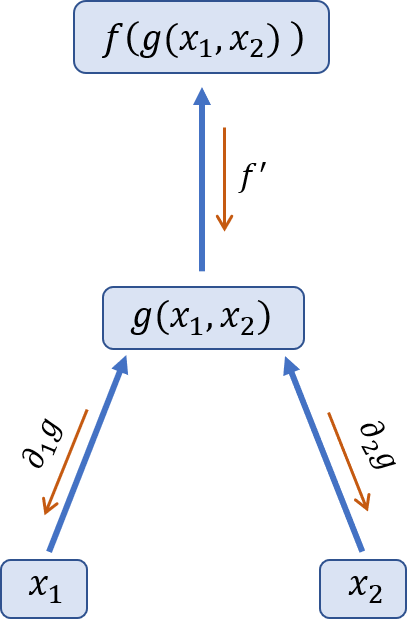
\includegraphics[height=1.3\textwidth]{Figures/automatic-differentiation}
	\end{minipage}\hfill
	\begin{minipage}{0.3\linewidth}
		\centering
		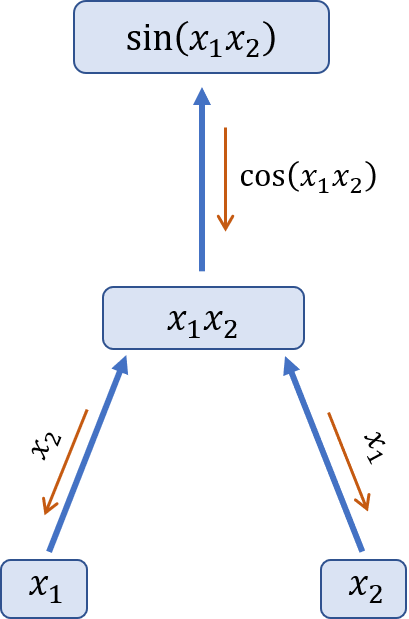
\includegraphics[height=1.3\textwidth]{automatic-differentiation2}
	\end{minipage}\hfill
	\begin{minipage}{0.3\linewidth}
		\centering
		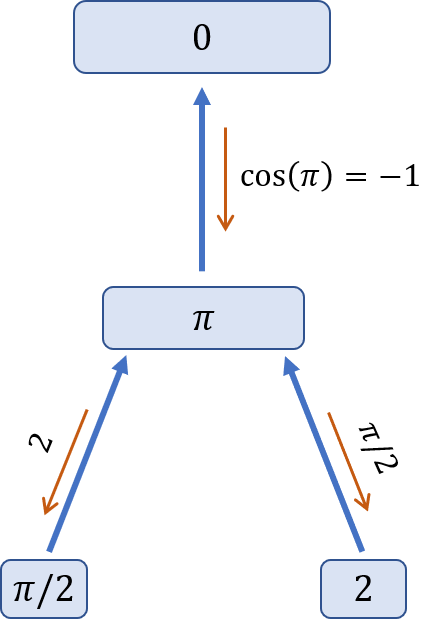
\includegraphics[height=1.3\textwidth]{automatic-differentiation3}
	\end{minipage}
	\caption{
		Examples of \ac{AD} in backpropagation mode.
		\textbf{(a)}
		Schematic representation of \ac{AD} of a function with one output and two inputs.
		Starting from numerical values for $x_1$ and $x_2$, one computes $g(x_1, x_2)$ and then $f(g(x_1, x_2))$.
		To get $\grad f(g(x_1, x_2))$, one then computes $f'(g(x_1, x_2))\partial_i g(x_1, x_2)$.
		Note that all components of this expression are known: $f'$ and $\partial_i g$ are known by assumption, and the value of $g(x_1, x_2)$ has been computed and cached in the forward propagation phase.
		\textbf{(b)} Example of application of \ac{AD} to compute the gradient of $\cos(x_1 x_2)$.
		\textbf{(c)} Using the same example function as (b), we give an example of the actual number computed at all stages when the inputs are $(x_1, x_2) = (\pi / 2, 2)$.
	}
	\label{fig:automatic-differentiation}
\end{figure*}

\subsection{Implementation details}
\label{subsec:implementation_details}

% Following the surge of interest in machine learning, and in particular deep learning, in the recent years
We used python as language of choice for the implementation of the supervised learning.
Being Python language of widespread use in the machine learning community, many libraries and frameworks are available to build computational graphs over which \ac{AD} can be used.
In particular, we used \textsc{Theano}~\cite{team2016theano}, together with the \textsc{QuTiP} library for the simulation of the dynamics of quantum systems~\cite{johansson2012qutip,johansson2013qutip}.
% The code used, together with a number of usage examples, is available on GitHub (\href{https://github.com/lucainnocenti/quantum-gate-learning}{Link}).

Our implementation allows the training of an arbitrary target gate, parametrised via a time-independent Hamiltonian $\mathcal H(\bs\lambda)$.
The parametrisation is completely arbitrary (provided the dependence on the parameters is linear), so that the Hamiltonian can be chosen as $\mathcal H(\bs\lambda)=\sum_i \lambda_i A_i$ for any set of matrices $A_i$ and number of parameters $\lambda_i$.
This is made possible by the flexibility of \ac{AD}, which allows to automatically build an efficiently differentiable computational graph, without needing to hardcode the structure of the Hamiltonian.

The goal of the algorithm is, given a target gate $\mathcal G$ and a parametrisation for the Hamiltonian $\mathcal H(\bs\lambda)$, find the $\bs\lambda_0$ such that $\exp(i\mathcal H(\bs\lambda_0))=\mathcal G$.
We use for the purpose mini-batch \ac{SGD} with momentum.
The \emph{mini-batch} version of \ac{SGD} involves computing the gradient, at every iteration, averaging over the gradients computed for a number of states.
Making such \emph{batches} of states larger or smaller allows to enhance or decrease the variance of the gradients with respect to the input state.
The use of \emph{momentum}~\cite{ruder2016overview,goh2017momentum} involves using a modified version of~\cref{eq:updating_rule}.
The updating rule is instead given by
\begin{equation}
\begin{aligned}
	\bs v &\to \gamma \bs v + \eta \grad_{\bs\lambda} \calF(\psi, \bs\lambda), \\
	\bs\lambda &\to \bs\lambda + \bs v,
\end{aligned}
\label{eq:updating_rule_momentum}
\end{equation}
where here $\eta$ is the \emph{learning rate} and $\gamma$ the \emph{momentum}.
The use of the auxiliary parameter $\bs v$ during the training discourages sudden changes of direction, and can make the training significantly more efficient~\cite{goh2017momentum}.

While the cost function $\calF$ is always real, some of the intermediate calculations needed to compute it involve complex numbers.
While this poses no fundamental problems, many of the \ac{ML} libraries do not support \ac{AD} over functions with complex inputs or outputs.
We worked around this problem using a similar trick to the one reported in~\cite{leung2017speedup}.
In particular, to use the existing framework, we mapped the problem into one involving only real numbers.
To do this, we map complex matrices into real ones via the bijection
$A\mapsto\mathfrak{Re}(A)\equiv\mathds1\otimes A_{R} - i \sigma_y\otimes A_{I}$,
where $A_R$ and $A_I$ are the real and imaginary parts of $A$, respectively.
At the same time, state vectors are to be mapped to
$\Psi\mapsto\mathfrak{Re}(\Psi)\equiv(\Psi_R, \Psi_I)^T$.
It is easy to verify that with this mapping
$A\Psi\mapsto\mathfrak{Re}(A\Psi)=\mathfrak{Re}(A)\mathfrak{Re}(\Psi)$,
so that all calculations can be equivalently be carried out with the real versions of matrices and vectors.

More specifically, the employed algorithm involves the following steps:
\begin{enumerate}
	\item Choose an initial set of parameters $\bs\lambda$ (randomly, or specific values if one has an idea of where a solution might be).
	A number of other hyperparameters have to be decided at this step, depending on the exact \ac{SGD} method used. In particular, for mini-batch \ac{SGD} with momentum and decreasing learning rate, one has to decide the momentum $\gamma$, the initial value of $\eta$, the rate at which $\eta$ decreases during the training, and the size $N_b$ of the batches of states used for every gradient descent step.
	\item Repeat the following loop $N_e$ times, or until a satisfactory result is obtained.
	Each such iteration is conventionally named an \emph{epoch}.
	Another hyperparameter to be chosen beforehand is the number of training states $N_{tr}$ to be used in each epoch.
	Once this is fixed, every epoch will involve a number $N_{tr}/N_e$ of gradient descent steps, each one using $N_e$ states for a single gradient calculation.
	$N_e$ random training states are sampled, to be used during the epoch.
	\begin{enumerate}
		\item Pick $N_b$ of the $N_e$ training states.
		\item Forward-propagate each state of the sample, and then backpropagate the gradients, thus computing the average gradient over the mini-batch $\grad_{\bs\lambda} \calF(\bs\lambda)$.
		\item Update the coupling strengths $\lambda$ as per~\cref{eq:updating_rule_momentum}.
		\item Return to point (a).
	\end{enumerate}
\end{enumerate}

\subsection{Results}
\label{subsec:numerical_results}

A sample of training results for Toffoli, Fredkin, and "double Fredkin" gates are given in Fig. 1 (a), (b), and (c) in the main text.
In~\cref{fig:toffoli_diagonal_parhistories,fig:fredkin_diagonal_parhistories,fig:doublefredkin_diagonal_parhistories} are shown the training histories of the parameters for eight different solutions for Toffoli, Fredkin and \emph{double Fredkin}, respectively.
These illustrate how quickly the networks converge for different initial values of the parameters.
In all the shown cases the target gates are obtained with unit fidelity up to numerical precision (that is, all fidelities are between $1-10^{-16}$ and $1$).
Different sets of optimisation hyperparameters are found to give acceptable solutions.
For the trainings shown in this paper we used a dynamically updated learning rate given, for the $k^{\text{th}}$ epoch, by $\eta=1/(1 + k \alpha)$ with the \emph{decay rate} $\alpha=0.005$.
The other hyperparameters were chosen as
$\gamma=0.5$, 
$N_b = 2$, $N_{tr} = 200$.
Different initial values for the parameters were tested, but in most cases we started the training with either vanishing or random (following a normal distribution) parameters.
For the training of the four-qubit gate we found the network to converge sooner to a solution when the parameters were initialised to a positive value (often with all parameters initialised to $4$).

In~\cref{fig:toffoli_fidVSpars,fig:fredkin_fidVSpars,fig:doublefredkin_fidVSpars} we report the behaviour of the fidelity upon changes of the learnt Hamiltonian parameters, for Toffoli, Fredkin and \emph{double Fredkin} gates, respectively.
As shown in these plots, the stability of the implemented gates with respect to variations of time and interactions values greatly varies between different solutions, as well as between different parameters in the same solutions.

To assess the feasibility of nontrivial gates in more restrictive experimental scenarios, we performed a systematic analysis of the reachability of Fredkin and Toffoli gates when allowing only for single-qubit and $X_i X_j+Y_i Y_j$ two-qubit interactions, and in the less restrictive setting of allowing for all $X_i X_j$ and $Y_i Y_j$ interactions.
The results are shown in~\cref{fig:fredkin_XY,fig:fredkin_XX,fig:toffoli_XX,fig:toffoli_XY}.
For the Fredkin gate, in the more restrictive $XX$ interactions setting, the biggest fidelity obtained was $\calF\simeq 0.94$, while when allowing for all $XX$ and $YY$ interactions the maximum fidelity obtained was $\calF\simeq0.999$.
For the Toffoli gate, the maximum fidelity obtained in the $XX$ scenario was $\calF\simeq0.94$ as well, while when allowing for all $XX$ and $YY$ interactions the best training results corresponded to $\calF\simeq 0.98$.
To have more consistent results, in all the training instances shown here all the hyperparameters, except for the interaction parameters' initial values, were chosen to have the same value.
In particular, each training instance was run for $200$ epochs, each one using $200$ random quantum states as inputs, divided in batches of $2$ elements.
This choice of hyperparameters is mostly empirical, and it is possible for different values to provide better results.

The above provides further evidence for the flexibility of the supervised learning approach, which can produce solutions with good fidelities even in more restrictive scenarios, closer to the capabilities of state of the art experimental architectures.
Furthermore, the values of the interaction strengths for many of the presented solutions are found to be compatible with the capabilities of state of the art circuit-QED architectures with gate times of the order of tens of nanoseconds~\cite{potocnik2018studying}.

Additional solutions and data, as well as the code used to produce them, is available in the GitHub repository
\href{https://github.com/lucainnocenti/quantum-gate-learning-1803.07119}{lucainnocenti/quantum-gate-learning-1803.07119}.
This repository contains all the code used to reproduce the solutions presented in this paper, as well as to train arbitrary gates on arbitrary numbers of qubits.
Even more generally, arbitrary (linearly) parametrised matrices can be used as training model, allowing a high degree of flexibility.

\begin{figure*}[htbp]
	\centering
	\begin{tikzpicture}
		\node[anchor=south west] (A) at (0, 0)%
			{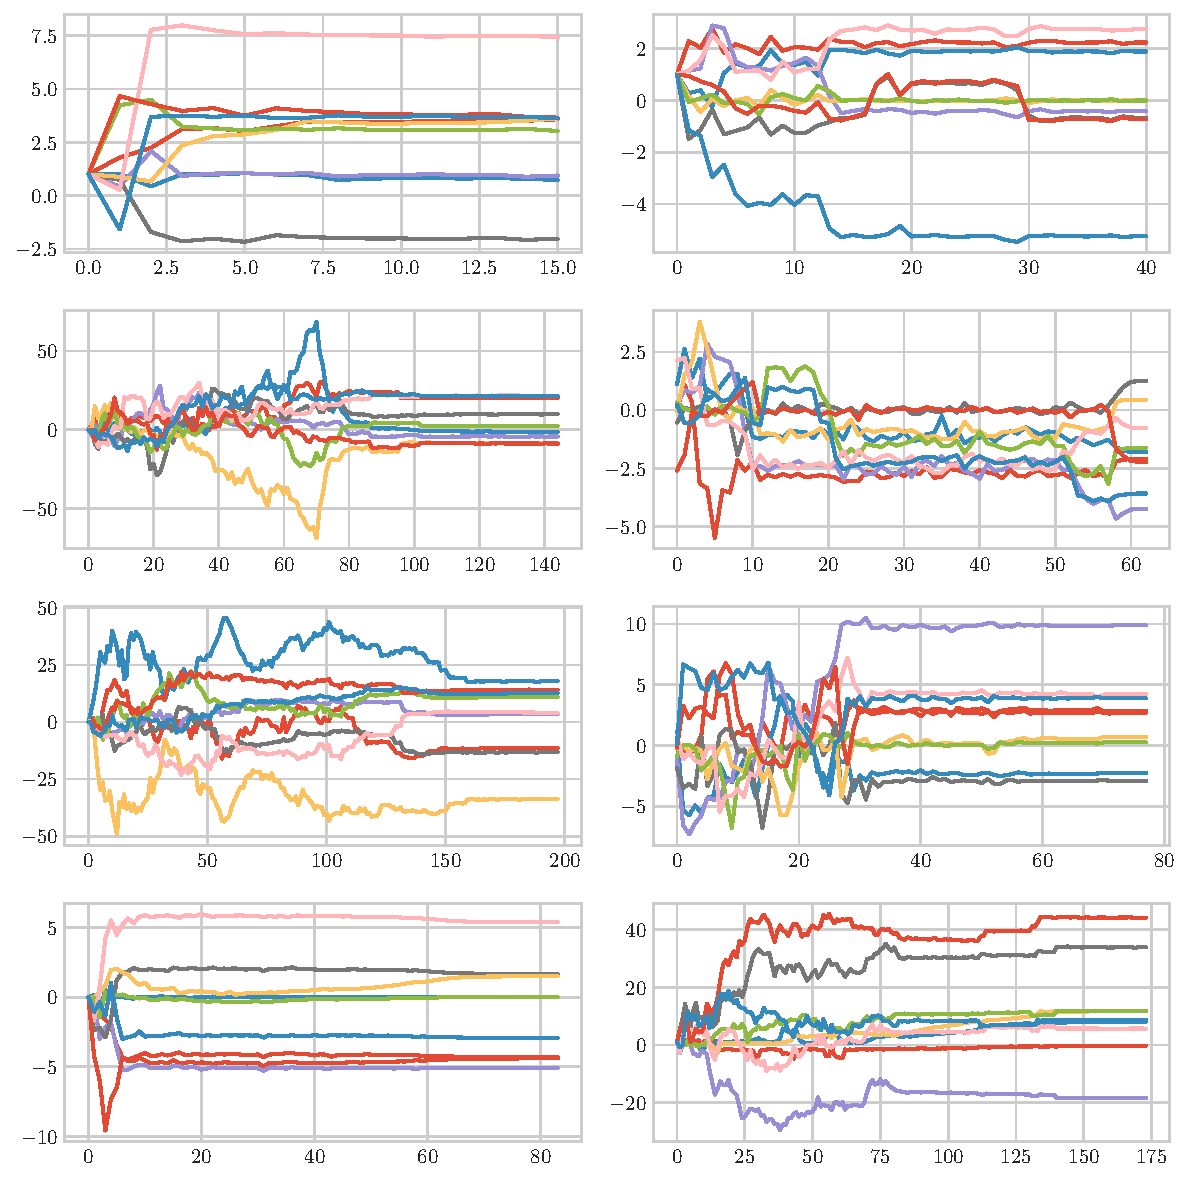
\includegraphics[width=.8\linewidth]{toffoli_diagonal_parhistories}};
		\node[above] at (4., -.2) {$t_e$};
		\node[above] at (11.5, -.2) {$t_e$};
	\end{tikzpicture}%
	% 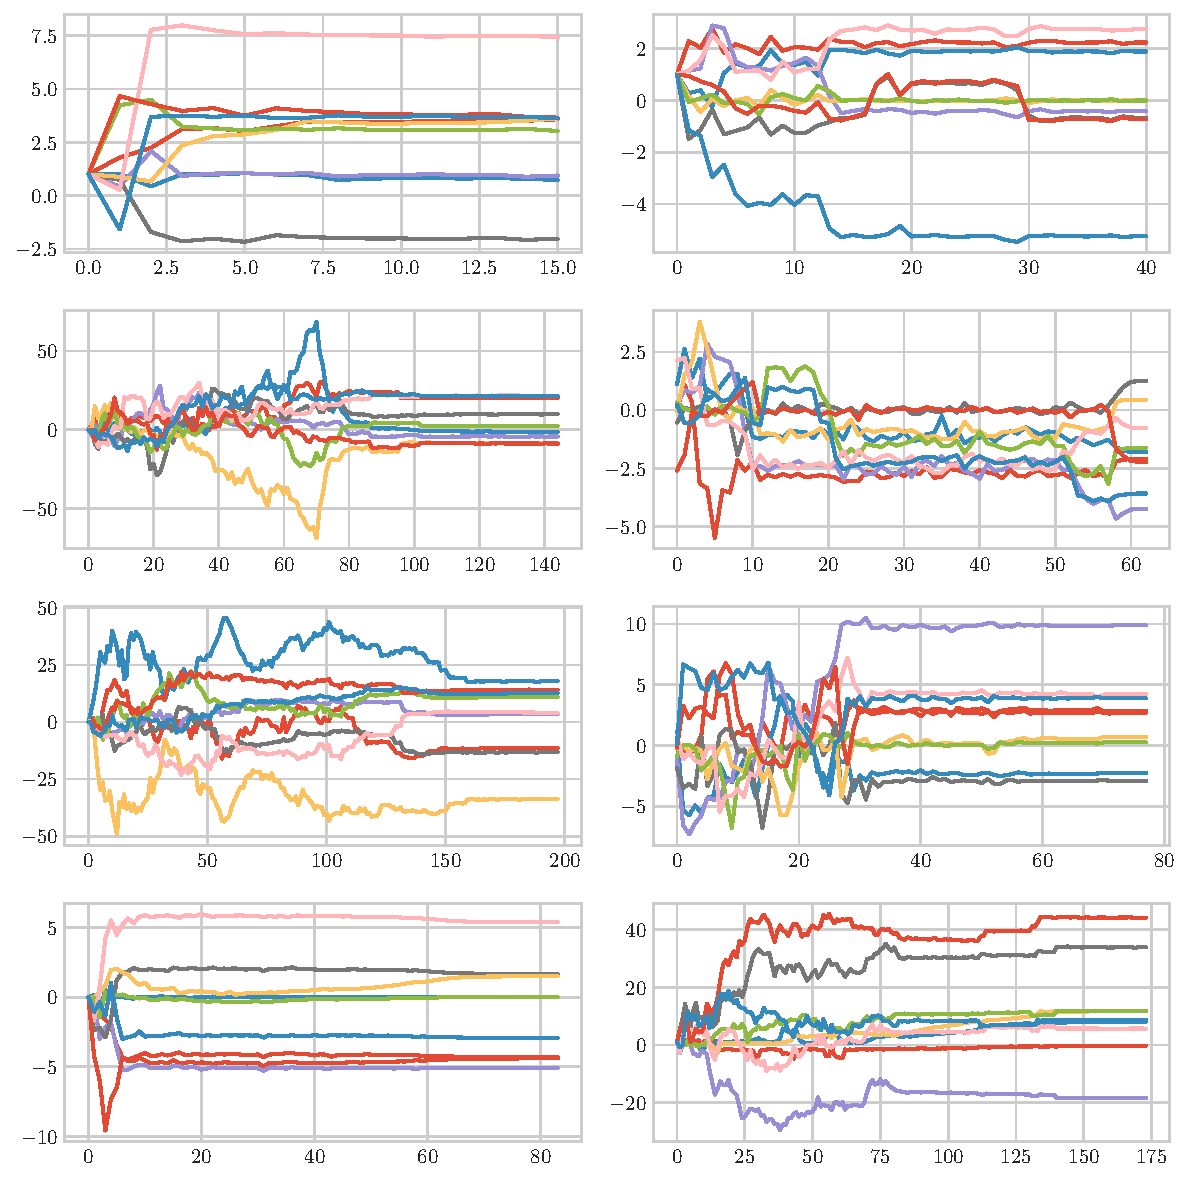
\includegraphics[width=.8\linewidth]{toffoli_diagonal_parhistories}
	\caption{
		Training histories for the \textbf{Toffoli} gate with only diagonal interactions.
		In each plot are reported the values of the $9$ network parameters during the training process, for each training epoch $t_e$.
		Each training process was left running until convergence to unit fidelity, therefore, the number of epochs in the horizontal axes differs for different trainings instances.
		The histories shown here correspond to training instances in which the parameters were initialised at various values, as seen from the leftmost values in each plot.
	}
	\label{fig:toffoli_diagonal_parhistories}
\end{figure*}

\begin{figure*}[htbp]
	\centering
		\begin{tikzpicture}
		\node[anchor=south west] (A) at (0, 0)%
			{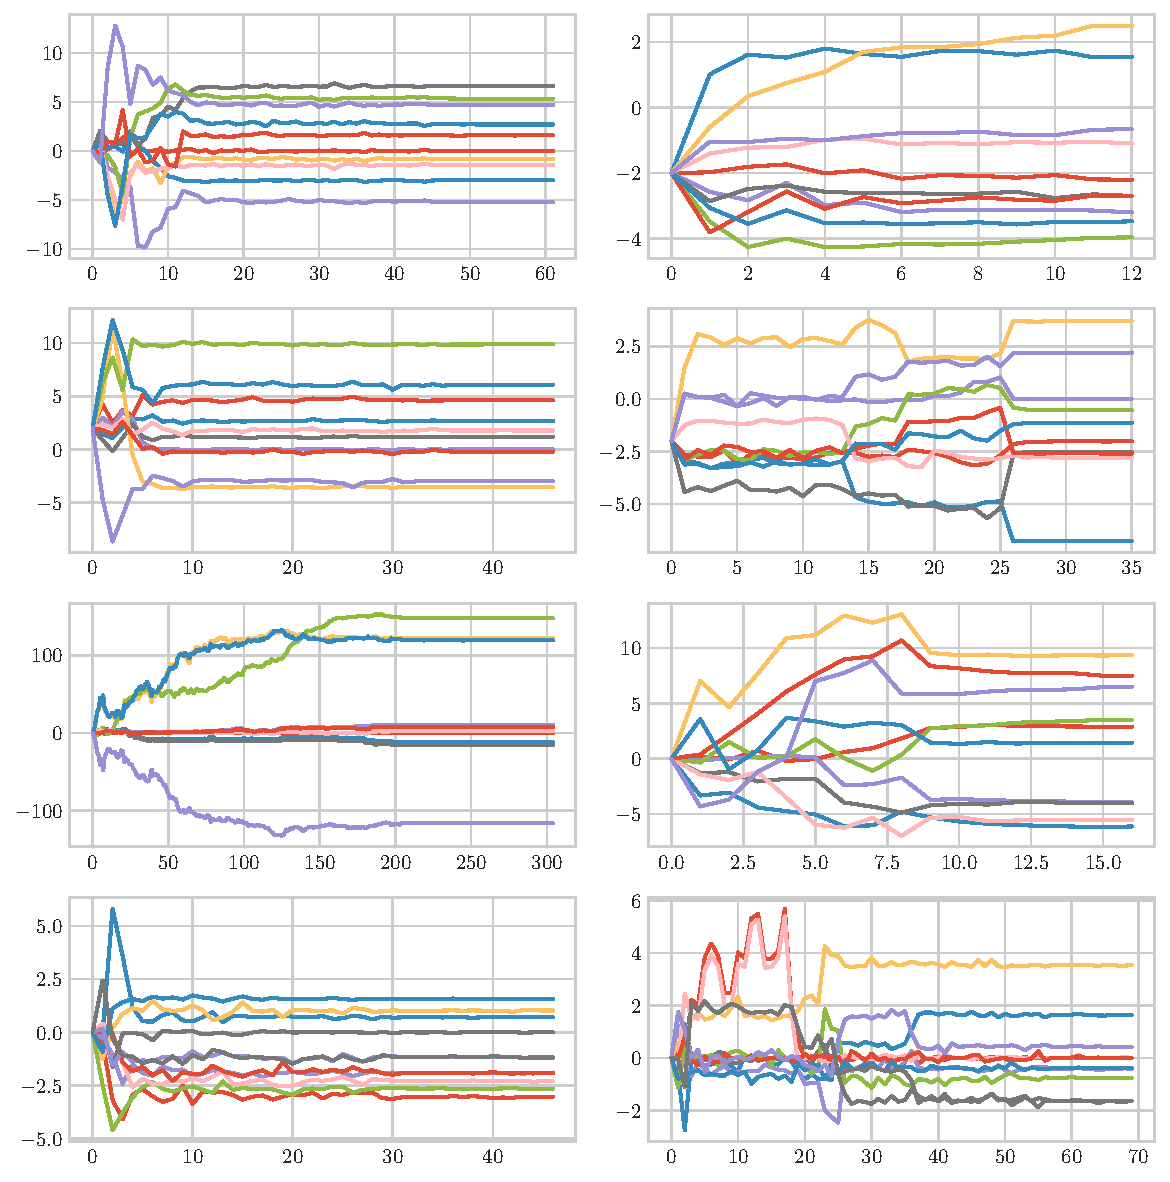
\includegraphics[width=.8\linewidth]{fredkin_diagonal_parhistories}};
		\node[above] at (4., -.2) {$t_e$};
		\node[above] at (11.5, -.2) {$t_e$};
	\end{tikzpicture}%
	% 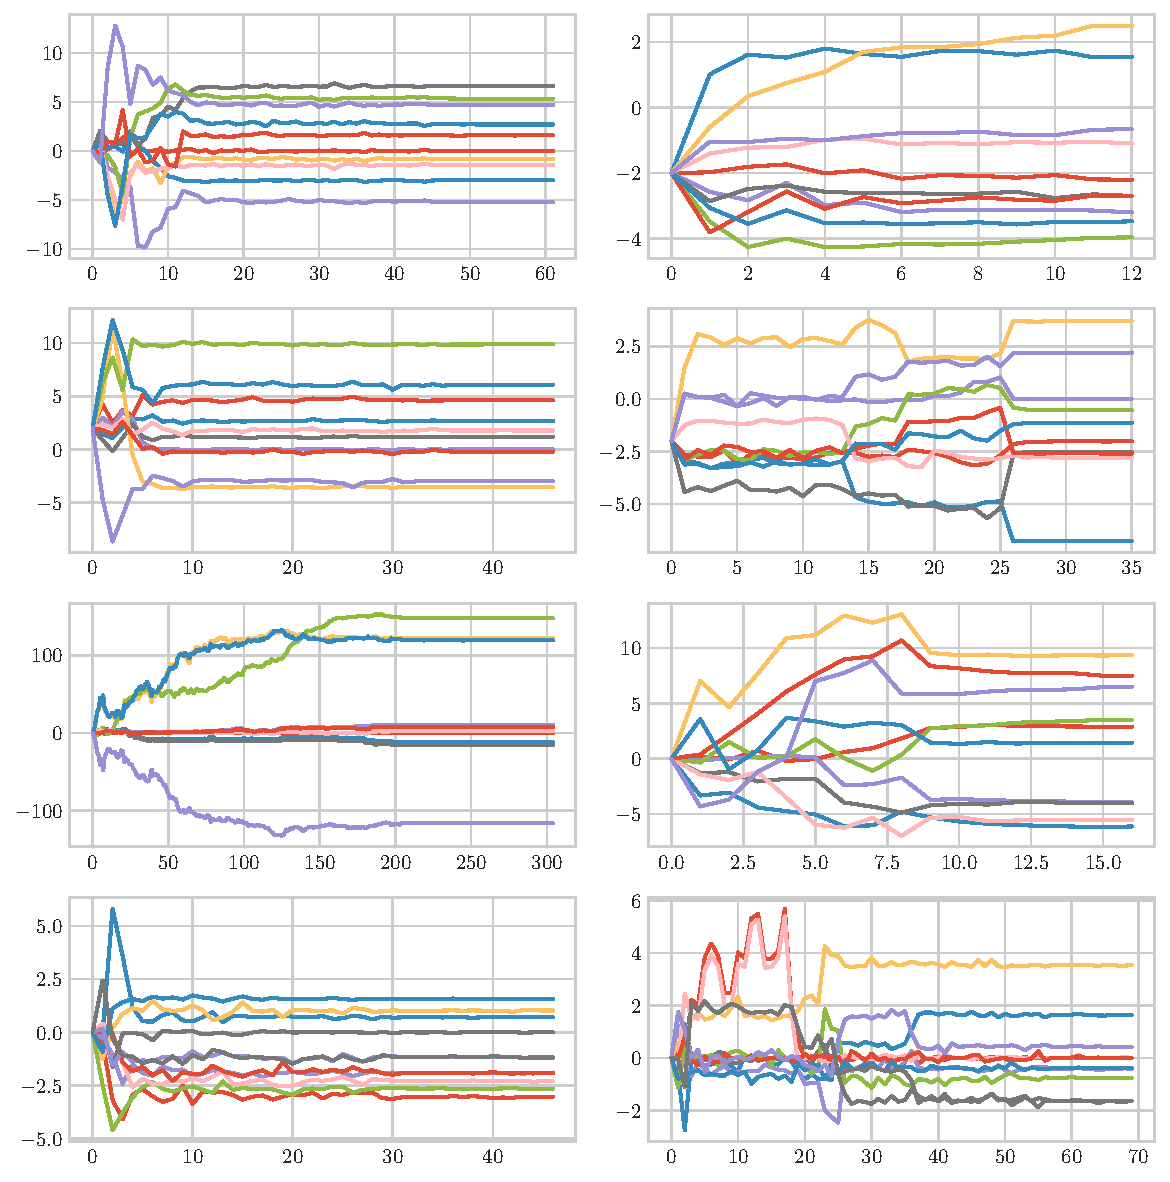
\includegraphics[width=.8\linewidth]{fredkin_diagonal_parhistories}
	\caption{
		Training histories for the \textbf{Fredkin} gate with only diagonal interactions.
		In each plot are reported the values of the $9$ network parameters during the training process, for each training epoch $t_e$.
		Each training process was left running until convergence to unit fidelity, therefore, the number of epochs in the horizontal axes differs for different trainings instances.
		The histories shown here correspond to training instances in which the parameters were initialised at various values, as seen from the leftmost values in each plot.
	}
	\label{fig:fredkin_diagonal_parhistories}
\end{figure*}

\begin{figure*}[htbp]
	\centering
	\begin{tikzpicture}
		\node[anchor=south west] (A) at (0, 0)%
			{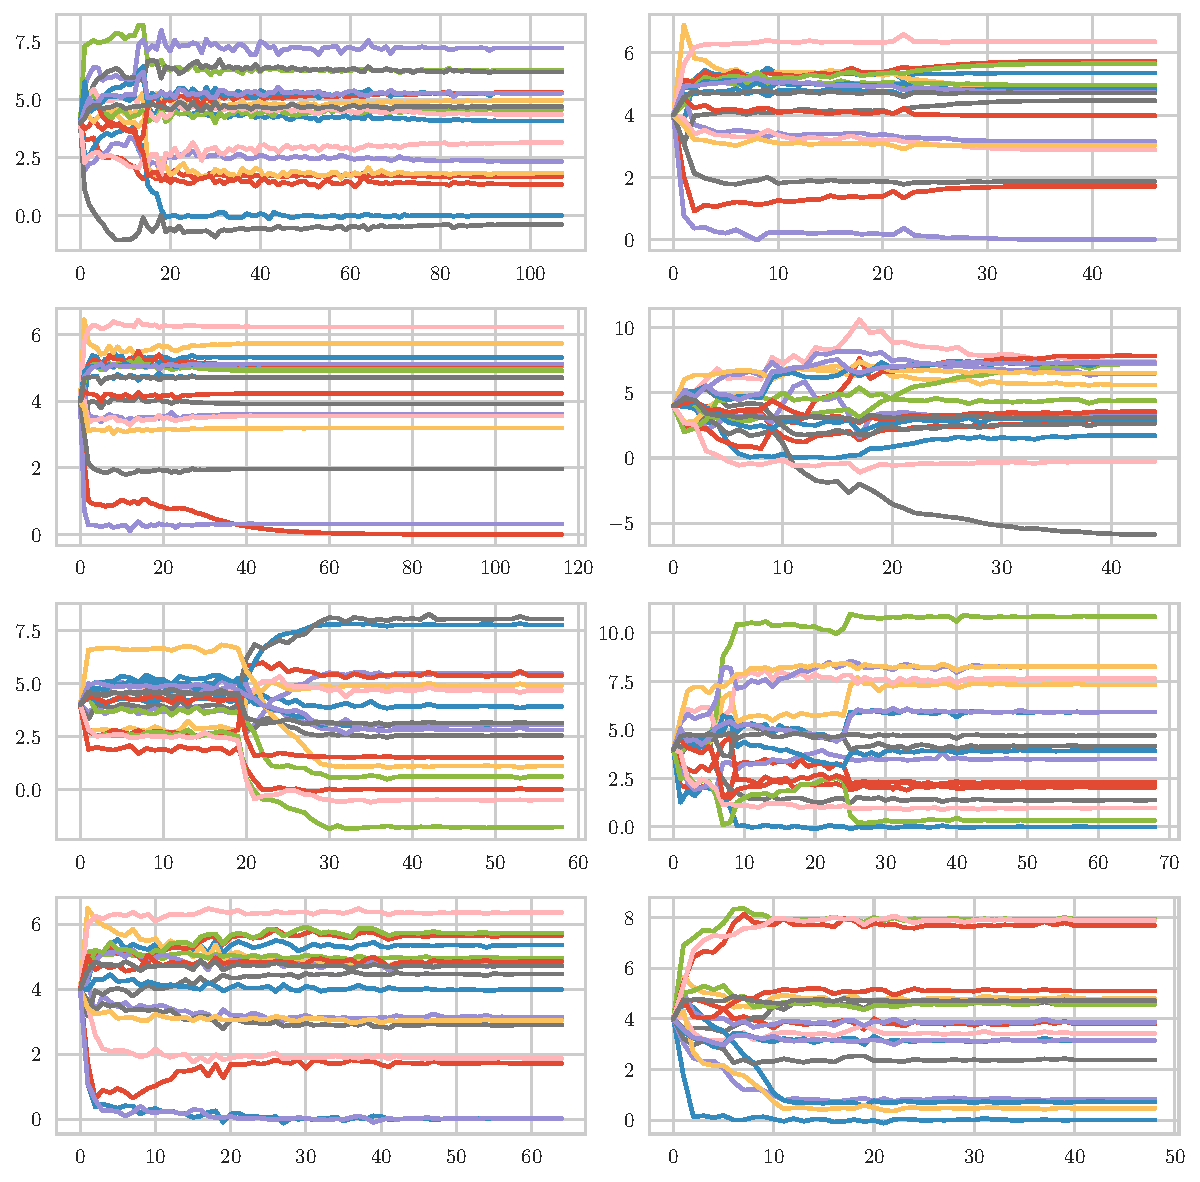
\includegraphics[width=.8\linewidth]{doublefredkin_diagonal_initvalues4_parhistories}};
		\node[above] at (4., -.2) {$t_e$};
		\node[above] at (11.5, -.2) {$t_e$};
	\end{tikzpicture}%
	% 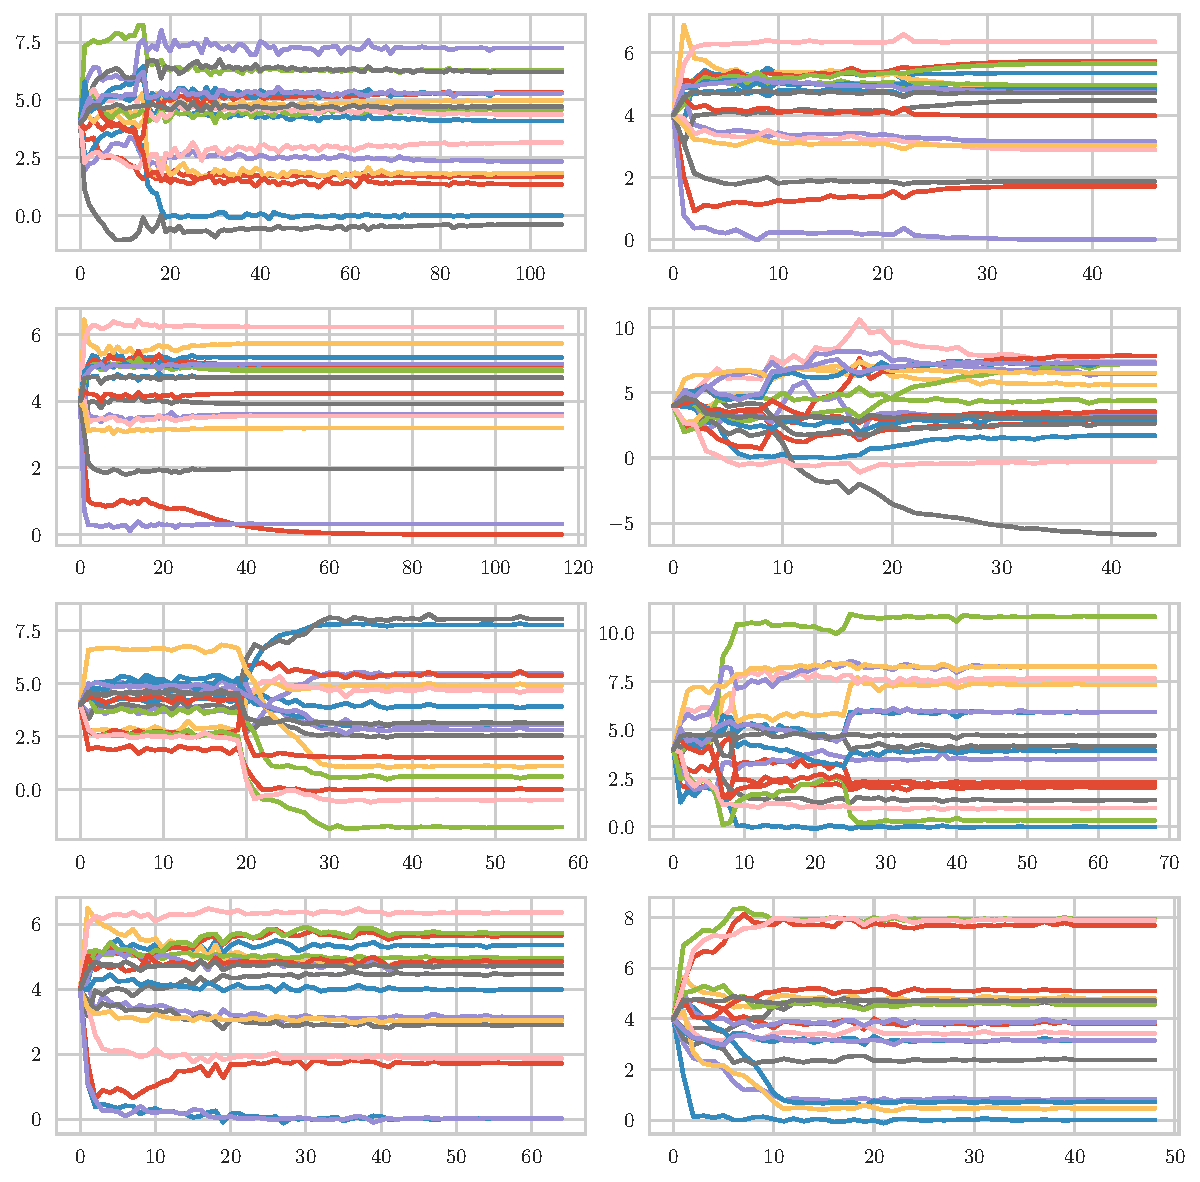
\includegraphics[width=.8\linewidth]{doublefredkin_diagonal_initvalues4_parhistories}
	\caption{
		Training histories for the \textbf{double-Fredkin} gate with only diagonal interactions.
		In each plot are reported the values of the $18$ network parameters during the training process, for each training epoch $t_e$.
		Each training process was left running until convergence to unit fidelity, therefore, the number of epochs in the horizontal axes differs for different trainings instances.
		All the histories shown here correspond to training instances in which the parameters were initialised to $4$.
	}
	\label{fig:doublefredkin_diagonal_parhistories}
\end{figure*}

\newcommand{\graphicswithlabel}[3]{%
	\begin{tikzpicture}
		\node[anchor=north west] (A) at (0, 0)%
			{\includegraphics[width=.48\linewidth]{#2}};
		\node[above] at (1.4, -.85) {\small\textbf{(#1)}};
		\node[above] at (4.6, -4.65) {#3};
		\node[above] at (1., -.2) {$\calF_\bslambda(\psi)$};
	\end{tikzpicture}%
}
\begin{figure*}[htbp]
	\centering
	\graphicswithlabel{a}{toffoli_fidVStime}{$\alpha$}\vspace{-6pt}
	\graphicswithlabel{b}{toffoli_fidVStime_wide}{$\alpha$}
	\graphicswithlabel{c}{toffoli_fidVSpar0}{$\lambda_1$}\vspace{-6pt}
	\graphicswithlabel{d}{toffoli_fidVSpar1}{$\lambda_2$}
	\caption{
		Fidelity $\calF_\bslambda(\psi)$ vs variations of $\bslambda$, for different test states, for the \textbf{Toffoli} gate. The five test states $\psi$ are sampled randomly.
		\textbf{(a)} Global relative variations of $\bslambda$, that is, plotting the fidelity against $\alpha\bslambda$ for $0.9 \le\alpha\le 1.1$.
		Note that this is equivalent to studying how the fidelity changes with respect to uncertainties in the evolution time, that is, how much does $\exp(i\HH t')$ differ from $\exp(i\HH t)$.
		\textbf{(b)} Same as \emph{(a)} but with $0\le\alpha\le 1.2$.
		\textbf{(c)} Plot of $\calF_\bslambda(\psi)$ against \emph{absolute} variations of a single element of $\bslambda$, in this case the first one, i.e. we take $\lambda_1\in[-10,10]$.
		\textbf{(d)} Like \emph{(c)} but for $\lambda_2$.
	}
	\label{fig:toffoli_fidVSpars}
\end{figure*}

\renewcommand{\graphicswithlabel}[3]{%
	\begin{tikzpicture}
		\node[anchor=north west] (A) at (0, 0)%
			{\includegraphics[width=.48\linewidth]{#2}};
		\node[above] at (1.4, -.85) {\small\textbf{(#1)}};
		\node[above] at (4.6, -4.65) {#3};
		\node[above] at (1., -.2) {$\calF_\bslambda(\psi)$};
	\end{tikzpicture}%
}
\begin{figure*}[htbp]
	\centering
	\graphicswithlabel{a}{fredkin_fidVStime}{$\alpha$}\vspace{-6pt}
	\graphicswithlabel{b}{fredkin_fidVStime_wide}{$\alpha$}
	\graphicswithlabel{c}{fredkin_fidVSpar0}{$\lambda_1$}\vspace{-6pt}
	\graphicswithlabel{d}{fredkin_fidVSpar3}{$\lambda_2$}
	\caption{
		Fidelity $\calF_\bslambda(\psi)$ vs variations of $\bslambda$, for different test states, for the \textbf{Fredkin} gate. The five test states $\psi$ are sampled randomly.
		\textbf{(a)} Global relative variations of $\bslambda$, that is, plotting the fidelity against $\alpha\bslambda$ for $0.9 \le\alpha\le 1.1$.
		Note that this is equivalent to studying how the fidelity changes with respect to uncertainties in the evolution time, that is, how much does $\exp(i\HH t')$ differ from $\exp(i\HH t)$.
		\textbf{(b)} Same as \emph{(a)} but with $0\le\alpha\le 1.2$.
		\textbf{(c)} Plot of $\calF_\bslambda(\psi)$ against \emph{absolute} variations of a single element of $\bslambda$, in this case the first one, i.e. we take $\lambda_1\in[-10,10]$.
		\textbf{(d)} Like \emph{(c)} but for $\lambda_2$.
	}
	\label{fig:fredkin_fidVSpars}
\end{figure*}

\renewcommand{\graphicswithlabel}[3]{%
	\begin{tikzpicture}
		\node[anchor=north west] (A) at (0, 0)%
			{\includegraphics[width=.48\linewidth]{#2}};
		\node[above] at (1.4, -.85) {\small\textbf{(#1)}};
		\node[above] at (4.6, -4.65) {#3};
		\node[above] at (1., -.2) {$\calF_\bslambda(\psi)$};
	\end{tikzpicture}%
}
\begin{figure*}[htbp]
	\centering
	\graphicswithlabel{a}{doublefredkin_fidVStime}{$\alpha$}\vspace{-6pt}
	\graphicswithlabel{b}{doublefredkin_fidVStime_wide}{$\alpha$}
	\graphicswithlabel{c}{doublefredkin_fidVSpar0}{$\lambda_1$}\vspace{-6pt}
	\graphicswithlabel{d}{doublefredkin_fidVSpar1}{$\lambda_2$}
	\caption{
		Fidelity $\calF_\bslambda(\psi)$ vs variations of $\bslambda$, for different test states, for the \textbf{double Fredkin} gate. The five test states $\psi$ are sampled randomly.
		\textbf{(a)} Global relative variations of $\bslambda$, that is, plotting the fidelity against $\alpha\bslambda$ for $0.9 \le\alpha\le 1.1$.
		Note that this is equivalent to studying how the fidelity changes with respect to uncertainties in the evolution time, that is, how much does $\exp(i\HH t')$ differ from $\exp(i\HH t)$.
		\textbf{(b)} Same as \emph{(a)} but with $0\le\alpha\le 1.2$.
		\textbf{(c)} Plot of $\calF_\bslambda(\psi)$ against \emph{absolute} variations of a single element of $\bslambda$, in this case the first one, i.e. we take $\lambda_1\in[-10,10]$.
		\textbf{(d)} Like \emph{(c)} but for $\lambda_2$.
	}
	\label{fig:doublefredkin_fidVSpars}
\end{figure*}


\newcommand{\traininggraphicswithlabel}[1]{%
	\begin{tikzpicture}
		\node[anchor=north west] (A) at (0, 0)%
			{\includegraphics[width=.85\linewidth]{#1}};
		\node[above] at (0, -.8) {$\barF$};
	\end{tikzpicture}%
}

\begin{figure*}[htbp]
	\centering
	% 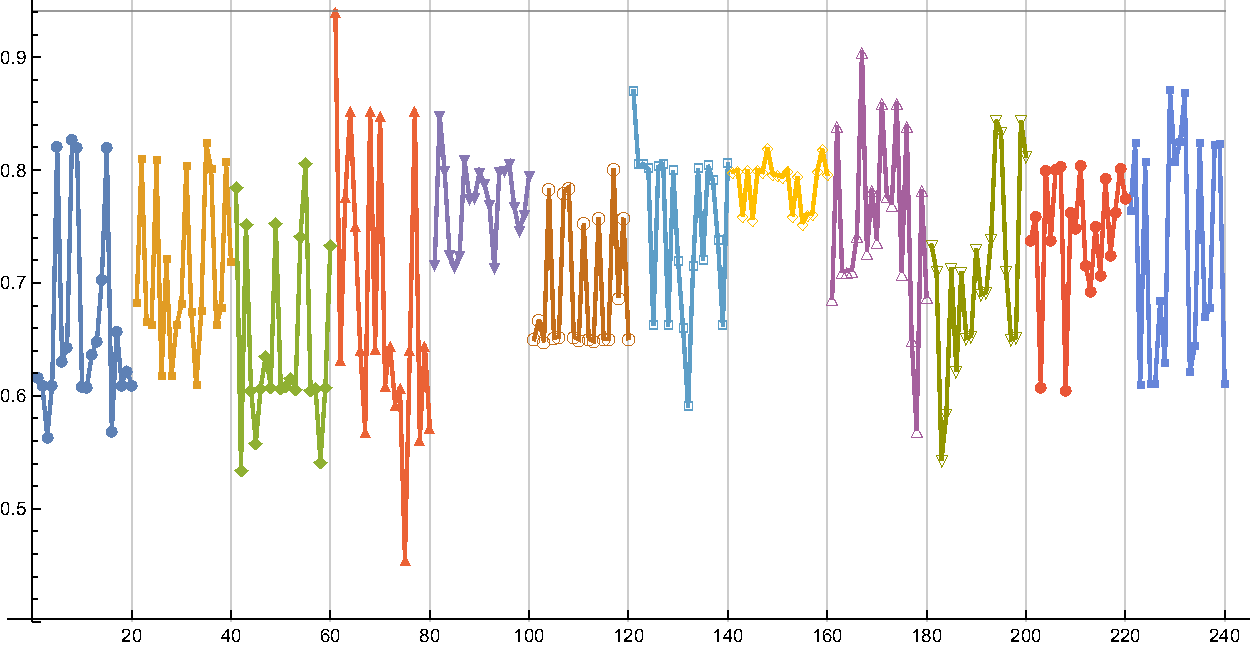
\includegraphics[width=.85\linewidth]{fredkin_noancillae_XXall.pdf}
	\traininggraphicswithlabel{fredkin_noancillae_XXall.pdf}
	\caption{
		Training results for the Fredkin gate with a generator containing one-qubit interactions and two-qubit interactions of the form $J_{ij}(X_i X_j + Y_i Y_j)$.
		Every point shows the final fidelity obtained at the end of a training procedure.
		The hyperparameters, as well as the total number of training iterations, are kept the same in all the training instances shown here.
		The initial parameters' values are the same within each horizontal sector, but changed between different sectors.
		The initial parameters' values within each sector have been chosen as all equal to $c$ (that is, $\lambda_i=c$ for all $i$). The values of $c$ are $0, 1,..., 10$, with $c=0$ in the leftmost sector and $c=10$ in the last to rightmost one.
		The rightmost sector contains the results of training attempts with the initial values chosen at random (that is, with $\lambda_i$ sampled according to the uniform normal distribution, independently for each $i$).
		The greatest reached fidelity, obtained with initial parameters' values $\lambda_i=3$, is $\calF\simeq0.94$.
	}
	\label{fig:fredkin_XX}
\end{figure*}

\begin{figure*}[htbp]
	\centering
	\traininggraphicswithlabel{fredkin_noancillae_XYall.pdf}
	\caption{
		Training results for the Fredkin gate with a generator containing all one-qubit interactions and two-qubit interactions of the form $J^{(1)}_{ij}X_i X_j + J^{(2)}_{ij}Y_i Y_j$.
		The initial conditions are chosen as in~\cref{fig:fredkin_XX}.
		The maximum fidelities obtained are $\calF\simeq0.999$, obtained in multiple instances $c=3$ and $c=4$ sectors.
	}
	\label{fig:fredkin_XY}
\end{figure*}

\begin{figure*}[htbp]
	\centering
	\traininggraphicswithlabel{toffoli_noancillae_XXall.pdf}
	\caption{
		Training results for the Toffoli gate with a generator containing all one-qubit interactions and two-qubit interactions of the form $J_{ij}(X_i X_j + Y_i Y_j)$.
		The initial conditions are chosen as in~\cref{fig:fredkin_XX}.
		The maximum fidelities obtained are $\calF\simeq0.94$, obtained in the $c=3$ sector.
	}
	\label{fig:toffoli_XX}
\end{figure*}

\begin{figure*}[htbp]
	\centering
	\traininggraphicswithlabel{toffoli_noancillae_XYall.pdf}
	\caption{
		Training results for the Toffoli gate with a generator containing all one-qubit interactions and two-qubit interactions of the form $J^{(1)}_{ij}X_i X_j + J^{(2)}_{ij}Y_i Y_j$.
		The initial conditions are chosen as in~\cref{fig:fredkin_XX}.
		The maximum fidelities obtained are $\calF\simeq0.98$, obtained in the $c=4$ and $c=5$ sectors.
	}
	\label{fig:toffoli_XY}
\end{figure*}

\subsection{Numerical approximate results in constrained scenarios}

% \EnableTOCUpdates


%!TEX root = ./Thesis.tex

\newcommand{\bsw}{{\bs{w}}}
\newcommand{\Utarget}{{\calU_{target}}}


\chapter{Porco dio}


\section{Introduction}
Machine learning techniques find fruitful application in several branches of quantum information theory~\cite{mehta2018highbias,spears2017contemporary,biamonte,petruccione,ciliberto2017quantum,perdomoortiz2017opportunities}.
Supervised learning, in particular, provides powerful tools to build algorithms able to pick up patterns from sets of pre-labelled data.
In the context of quantum information science, machine learning techniques have been showcased as a flexible tool to solve complex optimisation tasks in different areas~\cite{zdeborov2017machine,carrasquilla2017machine,carleo2017solving,van2017learning,schoenholz2016structural,torlai2018neural,rocchetto2017experimental,melnikov2018active,banchi2016quantum,fujita2018construction,innocenti2018supervised}.
In particular, supervised learning techniques were recently demonstrated to solve \emph{gate design} problems~\cite{banchi2016quantum,innocenti2018supervised}.

Here, by \emph{gate design problem} we mean the task of identifying a time-independent Hamiltonian generating a target evolution, under a series of restrictions imposed on the allowed Hamiltonian terms.
This problem is well suited for machine learning techniques because, while mathematically well-defined, it presents a complex and strongly context-depend phenomenology.
At the same time, the ability to implement non-trivial gates using time-independent dynamics and experimentally-feasible interactions is potentially of great interest for practical implementations of quantum algorithms.
It was recently shown in Ref.~\cite{innocenti2018supervised} that, by exploiting supervised learning techniques and ideas, it is possible to flexibly tackle arbitrary gate design problems.  A mathematical framework to further improve the efficiency of the numerics by providing improved ansatz for the optimisations can be formalised and used.
In this paper, we illustrate the methodology sketched in Ref.~\cite{innocenti2018supervised} and give further examples of time-independent Hamiltonians found via supervised learning optimisation, exploring cases in which ancillary qubits are used to catalyse the evolution, but are traced out at the end of the dynamics in such a way that the effective evolution over the system qubits is the desired one.

The remainder of this paper is organized as follows. In Sec.~\ref{sec:optimisation} we introduce the context of the problem that we address, stating the mathematical conditions that qualify a successful gate design (or synthesis). Sec.~\ref{learning} is dedicated to the illustration of the supervised learning approach that we use to tackle our problem. In Sec.~\ref{details} we discuss in details the stochastic momentum gradient descent approach that we choose to ensure the fulfilment of the mathematical conditions for gate design. Such methods are used in Sec.~\ref{results} to address quantitatively the training of a qubit network for the synthesis of three non-trivial three-qubit gates, including a half-adder and a quantum Fourier transform. We demonstrate that extremely high-quality gates can be synthesised using only evolutions coupling at most two qubits per time. Moreover, such restricted-resource designs are relatively stable against variations in the controlled parameters of the synthesis, which makes our approach robust, and potentially very interesting for implementation in a number of context, from superconducting quantum systems to trapped ions.
Finally, in Sec.~\ref{concl} we draw our conclusions.

\section{Optimisation of qubit networks}
\label{sec:optimisation}


Consider a set of qubits whose dynamics is described by the time-independent Hamiltonian $\HH_\bslambda=\sum_k \lambda_k A_k$, which is specified by the set of real parameters $\bslambda=\{\lambda_1,\lambda_2,\dots,\lambda_k,\dots\}$ and has been decomposed over the (Hermitian) operatorial basis $\{A_k\}$.
We consider some of the qubits of the set, say the first $M$ ones, as composing the \emph{system} ${\cal S}$ under investigation. The others embody a set  ${\cal A}$ of \emph{ancillary qubits}, whose collective initial state is set to be $\ket{\phi}_{\cal A}$.
We call $\ket\psi_{\cal S}$ the initial state of the system qubits, which we assume to be uncorrelated to the set of ancillae and will thus evolve as
\begin{equation}
	% \ketbra{\psi_{\on{out}}(t,\bslambda)} =
	\rho^{\cal S}_{\on{out}}(t, \bslambda) = %\rho_{\on{out}}(t\bslambda) =
	\Tr_\calA\left[\exp(it\HH_\bslambda)(\psi\otimes\phi)\right],
\end{equation}
where $\Tr_\calA$ denotes the partial trace of the ancillary qubits and we have used the shortcut notation
\begin{equation}
\exp(it\HH_\bslambda)(\psi\otimes\phi)=e^{it\HH_\bslambda}(\ket{\psi}\bra{\psi}_{\cal S}\otimes\ket{\phi}\bra{\phi}_{\cal A})e^{-it\HH_\bslambda}.
\end{equation}
Without loss of generality, in the following we can assume units such that $t=1$, so that the evolution time can be incorporated into a suitable rescaling of the the Hamiltonian parameters $\bslambda$. The evolved system state will henceforth be written as $\rho^{\cal S}_{\on{out}}(t,\bslambda)\equiv \rho^{\cal S}_{\on{out}}(\bslambda)$. Our goal is to find a set of parameters $\bslambda_0$ such that, for a given target evolution $\Utarget$, we have the successful gate synthesis $\Utarget=\exp(i\HH_{\bslambda_0})$.
This is equivalent to having
\begin{equation}
	% \ketbra{\psi_{\on{out}}(\bslambda)}=
	\rho^{\cal S}_{\on{out}}(\bslambda_0) =
	\Utarget(\ket{\psi}\bra{\psi}_{\cal S})\calU^\dagger_{target},\qquad \forall\ket{\psi}_{\cal S}.
\end{equation}
A natural way to quantify how much a given $\bslambda$ is close to the needed set $\bslambda_0$ is to use the state fidelity %function defined as
\begin{equation}
	\calF_\bslambda(\psi) ={}_{\cal S}\!\mel{\psi}{\calU_{target}^\dagger \rho_{\on{out}}^{\mathcal S}(\bslambda) \Utarget}{\psi}_{\cal S}.
	\label{eq:fidelity_definition}
\end{equation}
It then follows that
\begin{equation}
\label{condition}
\calF_{\bslambda_0}(\psi)=1\quad \forall\ket\psi \Leftrightarrow \exp(i\HH_{\bslambda_0})=\Utarget.
\end{equation}
Restricting ourselves to Hamiltonians having at most pairwise interactions, which are easier to implement in many experimental architectures, we can consider the following decomposition over the Pauli basis
\begin{equation}
	\HLambda = h_0 \mathds 1 + \sum h^\alpha_{i} \sigma_i^\alpha + \sum J_{ij}^{\alpha\beta} \sigma_i^\alpha \sigma_j^\beta.
	\label{eq:hamiltonian_atmostpairwise}
\end{equation}
Here, $i, j=1,...,N$ are indices for the qubits of the overall set (system and ancillae), $\alpha, \beta\in\{1,2,3\}$ identify the element of the Pauli vector ${\bm\sigma}=(\sigma^1,\sigma^2,\sigma^3)$ being considered (we use the correspondence $\sigma^1\rightarrow\sigma^x, \sigma^2\rightarrow\sigma^y, \sigma^3\rightarrow\sigma^z$), $J_{ij}^{\alpha\beta}$ is a coupling strength, and $\bslambda=\{h_0, h^\alpha_{i}, J_{ij}^{\alpha\beta}\}$.

Note that, for a given choice of $\Utarget$ and $\HLambda$, it is not known whether a solution to the question posed by Eq.~\eqref{condition} even exists.
% For example, it was until recently assumed that nontrivial three-qubit gates such as Toffoli and Fredkin could not be implemented with a time-independent dynamics without making use of ancillary qubits or higher-dimensional spaces~\cite{banchi2016quantum,zahedinejad2015highfidelity,zahedinejad2015highfidelity} (check).
Indeed, a simple parameter-counting argument shows it does not in general: not all possible evolutions produced using higher-order interactions can be generated when only one- and two-qubit couplings are available. A concrete example of the gate-synthesis problem discussed here is given by the implementation of a Toffoli gate~\cite{shi2002both} over a three-qubit network with a restricted set of interactions. Yet, Ref.~\cite{banchi2016quantum} has shown that the use of a single ancillary qubit catalyses the synthesis of three-qubit gates with the restricted resources mentioned above. Moreover,  it was recently shown~\cite{innocenti2018supervised} that the same task can be achieved \emph{without} ancillary qubits and under the stronger restriction of having available only \emph{diagonal} pairwise interactions. Whether a given gate can be realized with a specific time-independent set of operations remains an open question.

\section{Supervised learning of the Hamiltonian parameters}
\label{learning}

A standard approach to the design of Hamiltonians producing a target gate is the direct optimization of the average fidelity $\barF_\bslambda\equiv \int \calF_\psi \,d\psi$,
where the integral is performed over the set of all pure states $\ket\psi$.
Explicit closed expressions for $\barF_\bslambda$ are known~\cite{banchi2011nonperturbative,magesan2011gate,pedersen2007fidelity}, so that global optimisation algorithms can be applied directly.
However, the resulting complex parameter landscape makes such optimization inefficient. In order to avoid  the issues associated with global optimisation techniques, we thus resort to a different approach.

Instead of directly optimising $\barF_\bslambda$, we focus on single input states and optimise $\calF_\bslambda(\psi)$ for many different $\ket\psi$.
Formulated in this manner, the problem can be phrased in terms of supervised machine learning tasks, akin to the training of a neural network model.
Indeed, qubit networks can be trained to implement target evolutions just as neural network are trained to implement desired functional relationships.

One of the most used techniques to train neural network models is the so-called \ac{SGD}~\cite{wengert1964a,ruder2016an},
a workhorse of many state-of-the-art machine learning algorithms.
Given a parametrised functional relation $f_\bsw(\bsx)$, \ac{SGD} looks for sets of parameters $\bs w_0$ such that $f_{\bsw_0}(\bsx)$ is minimised for all $\bsx$.
This is done via the following iterative procedure: 1) choose a random input $\bsx_0$, 2) perform a few gradient descent steps over $\bsw$, and 3) go back to the first step, until a good result is obtained.
In this way some of the difficulties associated with local optimisation are avoided, because for every input $\bsx$ one has a different parameter landscape $\bsw\mapsto f_\bsw(\bsx)$ over which the gradient descent is performed.
This new parameter landscape does not in general have the same local minima as the previous ones, while on the other hand the global minimum is bound to be a minimum for all $\bsx$.
In the qubit network scenario that we are tackling, this translates into the fidelity being unitary for all $\ket\psi_{\cal S}$ only for the sets $\bslambda$ such that $\exp(i\HH_\bslambda)=\Utarget$.

Following the large body of research that the area of machine learning has seen in recent years~\cite{lecun2015deep,silver2016mastering}, a number of well-honed tools to efficiently tackle these kinds of tasks has been developed and made freely available.
In particular, software frameworks such as Theano~\cite{team2016theano}, TensorFlow~\cite{tensorflow2015-whitepaper} and PyTorch~\cite{paszke2017automatic} allow to efficiently train arbitrarily built models with state-of-the-art \ac{SGD} algorithms.
One particular aspect of these frameworks which allows to further speed-up the training procedure is that they allow to perform \emph{automatic differentiation}~\cite{wengert1964a,bartholomewbiggs2000automatic,baydin2015automatic} of arbitrary computations.
Automatic differentiation is a technique to efficiently compute, numerically, the gradient of an arbitrary multivalued function $f(\bs x)$, without using numerical approximation methods nor requiring the analytical expression of the gradient.
Such technique is especially valuable to speed-up \ac{SGD} optimisations, as it significantly decreases the cost of computing $\grad_\bsw f$.

\section{Implementation details}
\label{details}

We implement supervised learning of arbitrary qubit networks using Theano\cite{team2016theano}, a Python library for machine learning of widespread use.
More specifically, we use Theano to perform momentum-\ac{SGD}~\cite{ruder2016an} over the network parameters $\bslambda$, exploiting the automatic differentiation capabilities provided by Theano to speed-up the optimisation.
The implemented protocol can be summarized in the following steps
\begin{enumerate}
	\item Choose an initial set of parameters $\bs\lambda$.
	\item Generate a random set of input states $\ket{\psi_k}$, $k=1,..., N_b$, with $N_b$ the size of the mini-batches chosen beforehand.
	\item For each $k$, compute $\grad_{\bs\lambda} \mathcal F_{\bs\lambda}(\psi_k)$ using the automatic differentiation capabilities offered by Theano.
	\item Change the coupling strengths $\bs\lambda$ according to the chosen updating rule. A standard choice, adopted in this work, is momentum-SGD, which is characterised by the following updating rule:
	\begin{equation}
	\begin{aligned}
		\bs v &\to \gamma \bs v + \eta \grad_{\bs\lambda} \mathcal F_{\bs\lambda}(\psi_k), \\
		\bs\lambda &\to \bs\lambda + \bs v,
	\end{aligned}
	\end{equation}
	where the \emph{learning rate} $\eta$ and the \emph{momentum term} $\gamma$ are \emph{hyperparameters} that define the optimisation protocol.
	The value of the learning rate is also chosen to be decreasing with the iteration number.
	\item Return to point (2), until a satisfactory value of the fidelity is obtained.
\end{enumerate}
For the cost function $\mathcal F_\bslambda$ we use the expression given in~\cref{eq:fidelity_definition}, with a general Hamiltonian model with at most pairwise interactions, as given in~\cref{eq:hamiltonian_atmostpairwise}.
This means that, for example, to train the four-qubit networks implementing Half-adder and TofFredkin gates, we start with a general Hamiltonian like in~\cref{eq:hamiltonian_atmostpairwise} with $9$ parameters $h_i^\alpha$ for the single-qubit fields, plus $3\times9$ parameters $J_{ij}^{\alpha\beta}$ for the two-qubit interactions, amounting to a total of $36$ parameters to be trained.
The $h_0$ parameter can be left out of the training as it only amounts to an unobservable global phase.
A similar calculation tells us that for the $3+5$ network used to train the \ac{QFT} gate, a total amount of $276$ parameters are trained.

All the codes used to generate the results reported in this paper are freely available from Ref.~\cite{lucaarchivio}



\section{Results}
\label{results}
We trained qubit networks of various sizes to generate the \acf{QFT} over three qubits, a special doubly-controlled gate that shares characteristics with both Toffoli and Fredkin gate, to which we will refer to as \emph{TofFredkin} in the following, and the half-adder gate~\cite{barbosa2006quantum}.

The three-qubit \ac{QFT} transformation can be written as
\begin{equation}
\ac{QFT}\ket{a}_1\ket{b}_2\ket{c}_3=\frac{1}{\sqrt 8}\left(\ket0+e^{i\pi c}\ket1\right)_1\left(\ket0+e^{i\pi (b+\frac{c}{2})}\ket1\right)_2\left(\ket0+e^{i\pi (a+\frac{b}{2}+\frac{c}{4})}\ket1\right)_3
\end{equation}
with $\ket{k}_j$ the states of the system qubit $j=1,2,3$ ($k=a,b,c=0,1$).

We define the TofFredkin gate as the three-qubit transformation
\begin{equation}
{\cal U}_{\rm TF}=\ket{0}\bra{0}_1\otimes{\rm CNOT}_{23}+\ket{1}\bra{1}_1\otimes{\rm SWAP}_{23},
\end{equation}
which thus performs a CNOT (SWAP) gate on qubits $2$ and $3$, akin to a quantum Toffoli (Fredkin) gate, when the state of the control qubit 1 is $\ket{0}_1$ ($\ket{1}_1$).

Finally, the half-adder acts on a register of three qubits as
\begin{equation}
{\cal U}_{HA}={\rm CNOT}_{12}{\rm CCNOT}_{123},
\end{equation}
where ${\rm CCNOT}_{123}$ stands for the quantum Toffoli gate. When applied to a logical state $\ket{a}_1\ket b_2\ket c_3$, the half adder returns the state $\ket a_1\ket{a\oplus b}_2\ket{c\oplus{\rm carry}}_3$ with carry=0,1 the carry over of $a\oplus b$.

To assess the quality of the obtained gates we use the averaged gate fidelity $\barF(\mathcal E,\mathcal U)$, defined as
\begin{equation}
	\barF(\mathcal E, \calU) =
	\int d\psi \mel{\psi}{\calU^\dagger \mathcal E(\ketbra\psi)\calU}{\psi}.
	\label{eq:fidelity_definition}
\end{equation}
This quantity is used to characterize how close the action of a map $\mathcal E$ is to the action of a unitary $\U$.
The map is in our case the operation corresponding to the action of a unitary in the enlarged system+ancillae space, followed by tracing the ancillary qubits.
In our case, if $\tilde{\mathcal U}$ is the unitary acting on the full system+ancillae space, obtained from the learning procedure, then the map is defined as
${\mathcal E(\rho) = \Tr_A[\tilde{\mathcal U}(\rho\otimes\ketbra{0}) \tilde{\mathcal U}^\dagger]}$,
where $\ketbra{0}_A$ is the initial state of the ancillary system.
\Cref{eq:fidelity_definition} can be explicitly computed as
\begin{equation}
	\barF(\mathcal E,\U) = \frac{1}{d+1} \left[
		1 + \frac{1}{d}\sum_{ij}\mel{i}{\calU^\dagger \mathcal E(\ketbra{i}{j})\calU}{j}
	\right].
	\label{eq:fidelity_explicit_expr}
\end{equation}
In what follows, we use of~\cref{eq:fidelity_explicit_expr} to assess the quality of the reported results.

\Cref{fig:parameters} shows the sets of Hamiltonian parameters that were obtained through the training procedure, for each of these operations.
The TofFredkin gate was found with unit fidelity, up to numerical precision, using a single ancillary qubit. In~\cref{fig:toffredkin_fidVSpars} is shown how the fidelity varies with the Hamiltonian parameters. Fig.~\ref{fig:toffredkin_finalmatrix} reports the final matrix over the full four-qubit network.

In the case of the \ac{QFT}, we performed a series of training procedures with different sizes for the ancillary system, from the case of no ancilla to a maximum of five ancillary qubits being used.
We observed the best results when using 0, 3, and 5 ancillae, the average fidelities being $0.987$, $0.991$, and $0.988$ respectively.
It is important to note that due to the heuristic nature of the optimization method we employed, better results could be possible by using different initial conditions or  optimization parameters.
In~\cref{fig:parameters,fig:qft3q+5a_fidVSpars} we show the final parameters, and variation of final fidelities against the parameters, for the case of 5 ancillary qubits~\cite{seeRepoForQFTDetails}.

Finally, the half-adder gate was realized with average fidelity $\barF\simeq0.999997$ with a single ancilla.
Again, in~\cref{fig:halfadder_fidVSpars} is reported the behaviour of $\calF_\bslambda$ upon variations of $\bslambda$, and in~\cref{fig:halfadder_finalmatrix} we show the final unitary gate implemented over the full four-qubit network.

\Cref{fig:toffredkin_fidVSpars,fig:halfadder_fidVSpars,fig:qft3q+5a_fidVSpars} show the relative stability of the gates with respect to changes of the Hamiltonian parameters.
In particular, for TofFredkin and \ac{QFT}, the fidelity remains above $95\%$ upon a $25\%$ variation of the evolution time.
The half-adder appears to be less stable, but this is only consequence of the larger values of its interactions, as shown in~\cref{fig:parameters}(c).
Indeed, the hardness of tuning the Hamiltonian parameters with sufficient precision will vary strongly between different gates, as well as between different implementation of the same gate, and between different parameters in any given implementation.

These results provide further evidence in support of the power and flexibility of the supervised learning approach presented in~\cite{innocenti2018supervised,banchi2016quantum}, which clearly applies to the cases where ancillary degrees of freedom are exploited during the evolution.


\section{Conclusions}
\label{concl}

We have reported on strategies for supervised learning-assisted synthesis of multi-qubit quantum gates. The general scheme of our gate design is based on the use of a limited set of resources (such as two-qubit gates) that, in general, would not be sufficient for arbitrary gate design. However, the catalyst effect brought about by the use of machine learning -- specifically, stochastic momentum gradient descent -- is sufficient to overcome the limitation of our resources and deliver high-quality complex quantum gates. We have demonstrated the performance of our scheme by addressing the significant cases of a half-adder and a \ac{QFT} circuit. Moreover, we have shown the flexibility of our approach by addressing a novel type of gate that puts together the paradigmatic quantum Toffoli and Fredkin gates.

We believe that the proposed methodology will be able to significantly help in the task of designing complex evolutions suitable for the simulation of the dynamics of networks of information carriers, lowering the complexity associated with gate decomposition, and simply adopting well-known techniques of classical machine learning.


\chapter{Quantum Walks}
\label{Section:ChapAbbr}

% \BlankFootnote{Insert chapter footnote here.
% The chapter footnote could include citations to related publications by the author (``The material in this chapter was presented in part in ....'').}


\section{Che minchia so i QWs}
\section{E quindi?}
\section{Quantum state engineering with QWs}
\section{Synthesizable states characterisation work}
\section{VVB characterisation work}


\label{Section:ChapAbbr:Introduction}

% \EnableTOCUpdates

%!TEX root = ./Thesis.tex

\chapter{Experimental engineering of qudit states}
\label{chapter:experimental_engineering_qudits}

\tmpHeading{Summary of the work} In this chapter we present an experimental implementation of the state engineering scheme discussed in~\cref{chapter:quantum_walks}, leveraging the \emph{coin space} of a \ac{QW} as an auxiliary degree of freedom to engineer target qudits.
We use for the purpose an experimental apparatus implementing time-dependent \acp{QW} in the polarisation and \ac{OAM} degrees of freedom~\cite{zhang2010implementation,goyal2013implementing,cardano2015quantum}, exploiting the so-called \acp{QP}~\cite{marrucci2006optical} to implement the controlled-shift QW operation.
To benchmark and showcase the potential of the apparatus, we demonstrate the engineering of several classes of states.
The work described in this chapter can be found in~\cite{giordani2019experimental}.

% \tmpHeading{Why \ac{OAM}?} \acf{OAM} allows to encode high-dimensional quantum states in spatially localised photons. Moreover, \acp{QP} intertwine the polarisation and \ac{OAM} degrees of freedom of light, thus allowing more complex dynamics exploiting both types of degrees of freedom.
% With this apparatus, $n$ \ac{QW} steps require $\mathcal O(n)$ optical components -- one \ac{QP} and a few waveplates for each step -- thus making the scheme efficient. Moreover, by having access to fast-enough optical switches and fastly tunable \acp{QP} and waveplates, it is in principle possible to use a single \ac{QP} and waveplate for arbitrary many steps, by having the light pass through the same optical elements multiple times \highlight{(mmmh)}.
% in \emph{light} of the favourable scaling of the number of optical elements with the size of the walk~\cite{reck1994experimental,clements2016optimal}. Moreover, the scheme allows for the full control of the coin operation that is key to the walk implementation of the walk.


% \tmpHeading{What will we conclude from the chapter?}
% The quality of the generated states and the feasibility of the experimental protocol that we have put in place, demonstrate the effectiveness of a hybrid platform for quantum state engineering. Such platform holds together a programmable quantum system, the photonic \ac{QW} in the angular momentum, and classical optimisation algorithms to effectively generate a given target \highlight{???}.

\tmpHeading{Chapter outline}
\Cref{sec:expQWs:OAMintro} gives a brief overview of \ac{OAM} and \acp{VVB}.
In~\cref{sec:expQWs:experimental_apparatus} we describe how the protocol put forward in~\cref{chapter:quantum_walks} is used to experimentally engineer six-dimensional qudits.
We then present and discuss the experimental results in~\cref{sec:expQWs:results}, and give our conclusions and outlook in~\cref{sec:expQWs:conclusions}.


\section{Orbital angular momentum of light}
\label{sec:expQWs:OAMintro}

\tmpHeading{Orbital angular momentum of light}
Electromagnetic fields carry angular momentum \cite{jackson1999classical}.
Classically, the angular momentum density of an electromagnetic field is given, up to constants, by
$\bs M =\bs r\times(\bs E\times \bs B)$. This can be decomposed in an \emph{intrinsic} component, the so-called \emph{spin angular momentum}, and an \emph{extrinsic} one, its \ac{OAM}: $\bs M=\bs S+\bs L$, albeit this decomposition is not gauge invariant, and thus not always sensible~\cite{ohanian1986what,cameron2015azimuthal}.
The spin angular momentum is often understood to be due to an internal degree of freedom of the fields, and is what we usually refer to as the \emph{polarisation} of the field. The OAM is instead a property of the spatial structure of the field.
A first experimental demonstration of transfer of \emph{spin} angular momentum of light to matter was given in~\cite{beth1936mechanical}. A few decades later, Allen and collaborators showed that specific types of laser modes also carry an amount of \emph{orbital} angular momentum, due to the nontrivial phase structure of their transverse beam profile~\cite{allen1992orbital}.
Despite the Poynting vector $\bs E\times \bs B$ always pointing in the propagation direction for transverse beams, and thus $\bs r\times(\bs E\times\bs B)$ being vanishing in such direction, Allen et al. realised that the TEM$_{p\ell q}$ laser modes are in general \emph{not} transverse, but rather have a component in the propagation direction. Because of this, they could show that, for this fields, $\bs M$ has a component in the propagation direction, and thus the beams carry OAM.
Since Allen's groundbreaking work, the OAM of light found several applications in quantum information theory~\cite{allen1999orbital,padgett2004lights,barnett2007orbital,molina-terriza2007twisted,franke-arnold2008advances,yao2011orbital,padgett2017orbital,erhard2017twisted,cozzolino2019highdimensional}.
In particular, OAM of photons has been used for communication protocols~\cite{langford2004measuring}, quantum metrology~\cite{dambrosio2013photonic}, as well as to study quantum correlations~\cite{leach2010quantum,mair2001entanglement,vaziri2002experimental,dada2011experimental,pors2011highdimensional,fickler2012quantum,malik2016multiphoton}.
% that is proportional to $\ell$, which is the quantum number that determines the azimuthal phase profile of the field.
The most common types of helical laser beams carrying OAM are \ac{LG} modes, here denoted with $LG_p^\ell$. These are solutions of the Helmholtz equation in cylindrical coordinates in the paraxial approximation. LG modes are defined by the two quantum numbers $p$ and $\ell$, respectively characterising the radial and azimuthal structure of the mode. A characteristic feature of these beams is their azimuthal phase dependence: $LG_p^\ell\sim e^{i\ell\phi}$ with $\phi$ the azimuthal coordinate in the plane transverse to the propagation direction. LG modes carry an integer amount of OAM.
In~\cref{fig:expQWs:LG_profile_L0P2Z03,fig:expQWs:LG_profile_L1P2Z03} we give two examples of the transverse intensity profile of LG modes with different azimuthal quantum numbers $\ell$.
% ~\cite{mair2001entanglement,kwiat1993highvisibility,howell2004realization,}

\tmpHeading{Coupling OAM with polarisation}
While in vacuum, the spin and orbital components of the angular momentum are conserved, this ceases to be the case in inhomogeneous, anisotropic media. This makes it possible to devise devices which couple spin and OAM of impinging light. One such device is the so-called \acf{QP}~\cite{marrucci2006optical}.
When polarisation and OAM are coupled, we talk of a \acf{VVB}~\cite{cardano2012polarization}.
VVBs find application in multiple fields of classical and quantum optics~\cite{marrucci2011spintoorbital,cozzolino2019highdimensional,cardano2015spin–orbit,rubinsztein-dunlop2016roadmap}.
In the context of quantum information, VVBs have been studied for their peculiar entanglement structure~\cite{dambrosio2016entangled}, quantum communication and cryptography~\cite{vallone2014freespace,wang2015quantum,mirhosseini2015highdimensional,willner2015optical,malik2016multiphoton,sit2017highdimensional,cozzolino2019orbital,cozzolino2019aircore}, quantum walks~\cite{zhang2010implementation,goyal2013implementing,cardano2015quantum}, quantum simulation~\cite{cardano2016statistical,cardano2017detection}, and quantum memories~\cite{parigi2015storage}.

\tmpHeading{Encoding information in VVBs}
Despite their potential, decoding information stored into VVBs remains nontrivial. Efficient \ac{OAM}-demultiplexing requires interferometry~\cite{leach2002measuring,slussarenko2010polarizing,bauer2013nanointerferometric} or spatial filtering~\cite{berkhout2010efficient,bolduc2013exact,malik2014direct},
and these introduce detrimental effects of loss and noise~\cite{qassim2014limitations}.
More generally, the state tomography of such high-dimensional states is always challenging~\cite{paris2004quantum,banaszek2013focus}.
% Moreover, the challenge of performing state tomography of such high-dimensional states can hardly be overestimated
The design and demonstration of reliable techniques to generate and classify \acp{VVB} is thus highly desirable. Previous efforts to find novel platforms to manipulate VVBs~\cite{liu2016generation,ndagano2017creation,cardano2015spin–orbit,rubinsztein-dunlop2016roadmap},
include integrated photonics~\cite{chen2018mapping,cai2012integrated,liu2017direct} and plasmonic metasurfaces~\cite{karimi2014generating,yue2016vector}.


% \begin{figure}[tb]
% 	\centering
% 	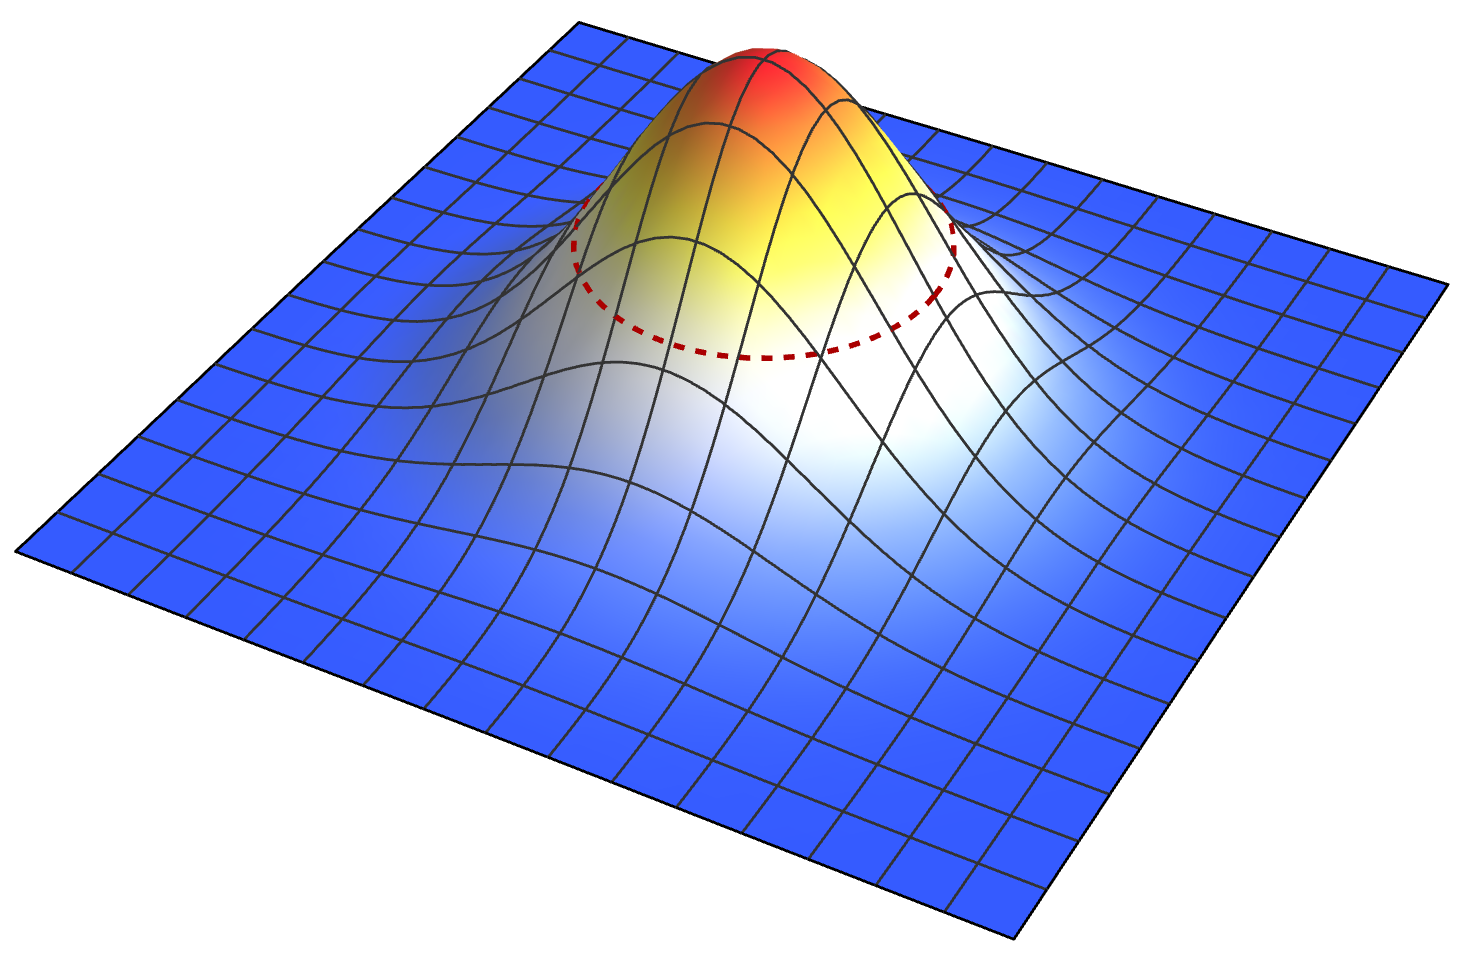
\includegraphics[width=.7\linewidth]{Figures/OAM/GaussianBeam2.png}
% 	\caption{%
% 		Gaussian beam
% 	}
% 	\label{fig:expQWs:gaussian_beam}
% \end{figure}

% \begin{figure}[tb]
% 	\centering
% 	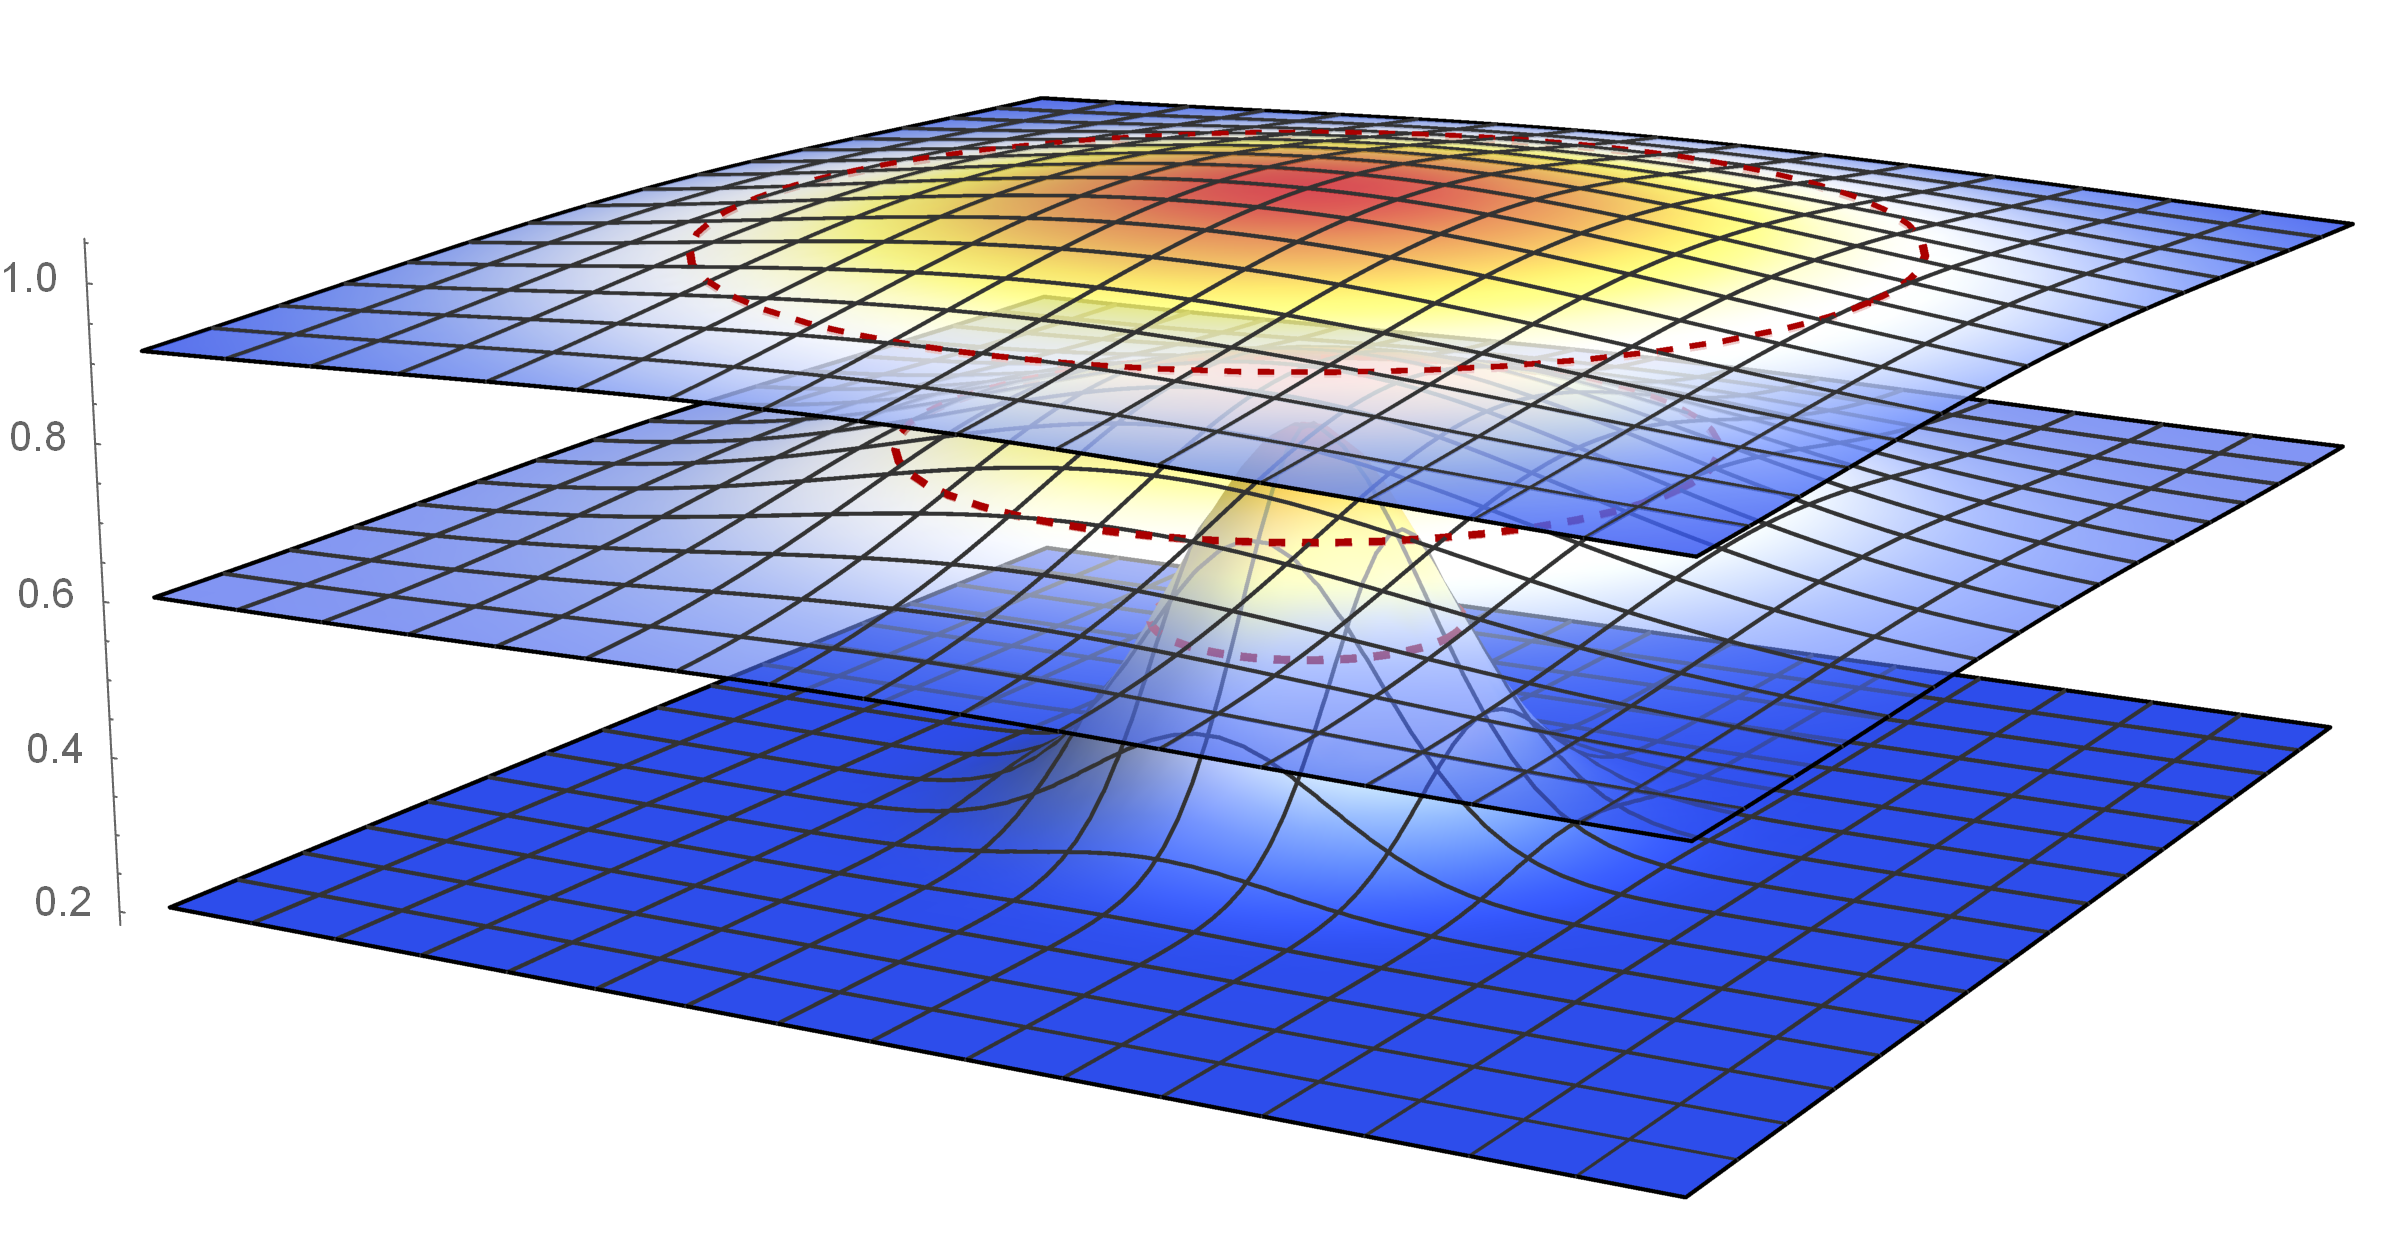
\includegraphics[width=.7\linewidth]{Figures/OAM/GaussianBeamDispersion.png}
% 	\caption{%
% 		Gaussian beam
% 	}
% 	\label{fig:expQWs:gaussian_beam}
% \end{figure}

\begin{figure}
    \centering
    \begin{minipage}{0.45\textwidth}
        \centering
        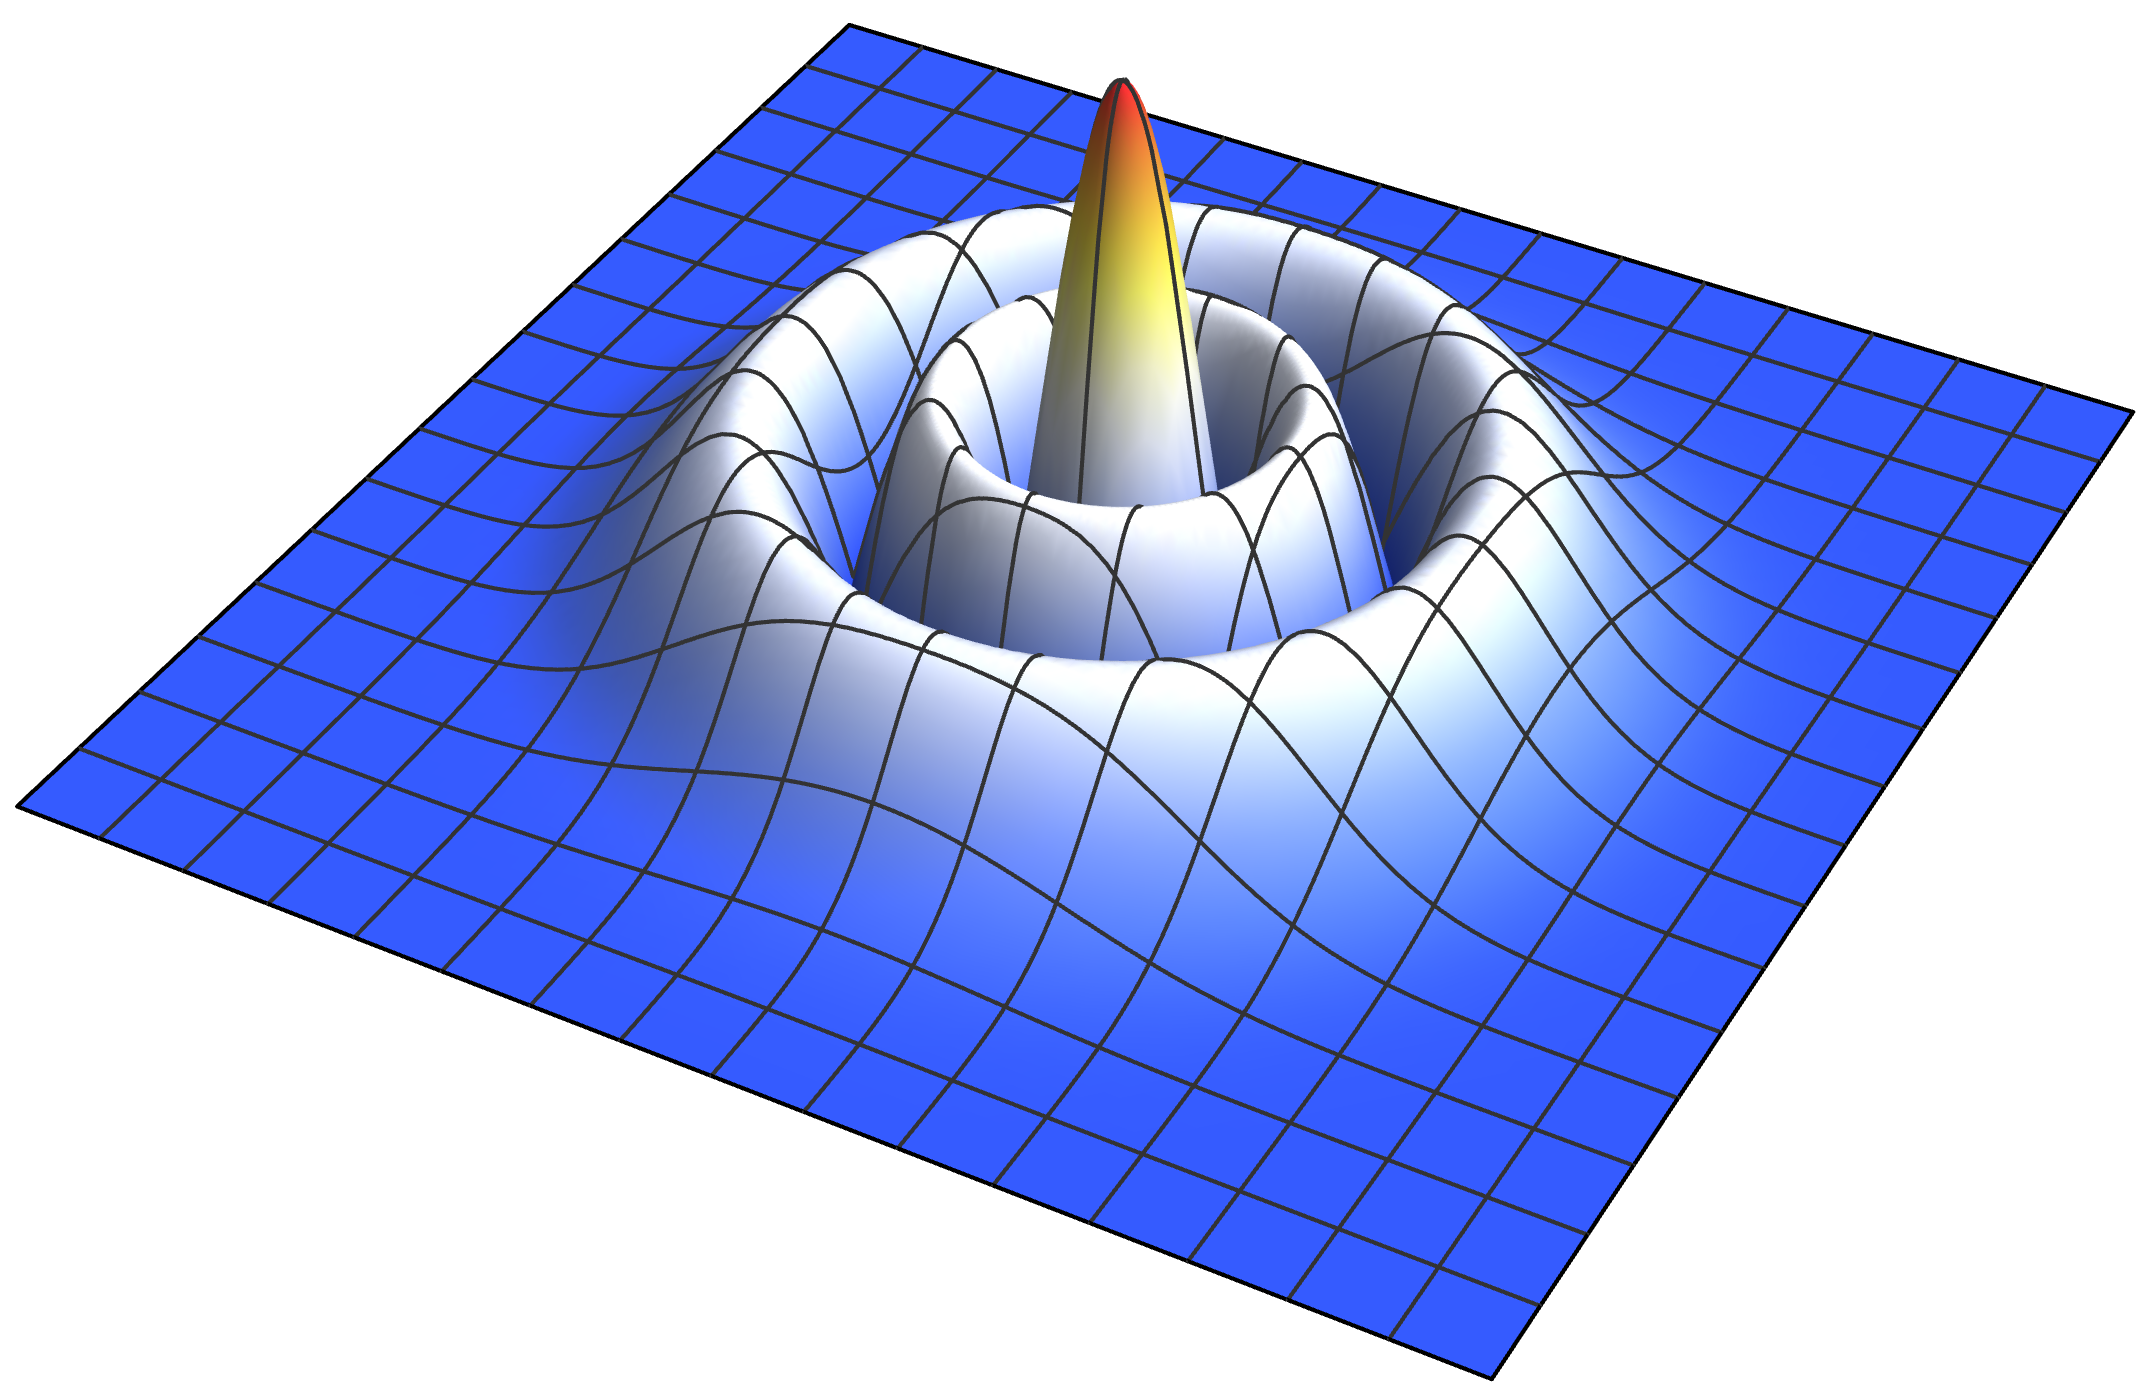
\includegraphics[width=1\textwidth]{Figures/OAM/LGBeamProfile_L0P2Z03.png} % first figure itself
        \caption{
        	Transverse profile of an OAM state with $\ell=0, p=2$.
        	% Transverse profile of an OAM state with $\ell=0, p=2, z=3$.
        }
        \label{fig:expQWs:LG_profile_L0P2Z03}
    \end{minipage}\hfill
    \begin{minipage}{0.45\textwidth}
        \centering
        \vspace{-30pt}%
        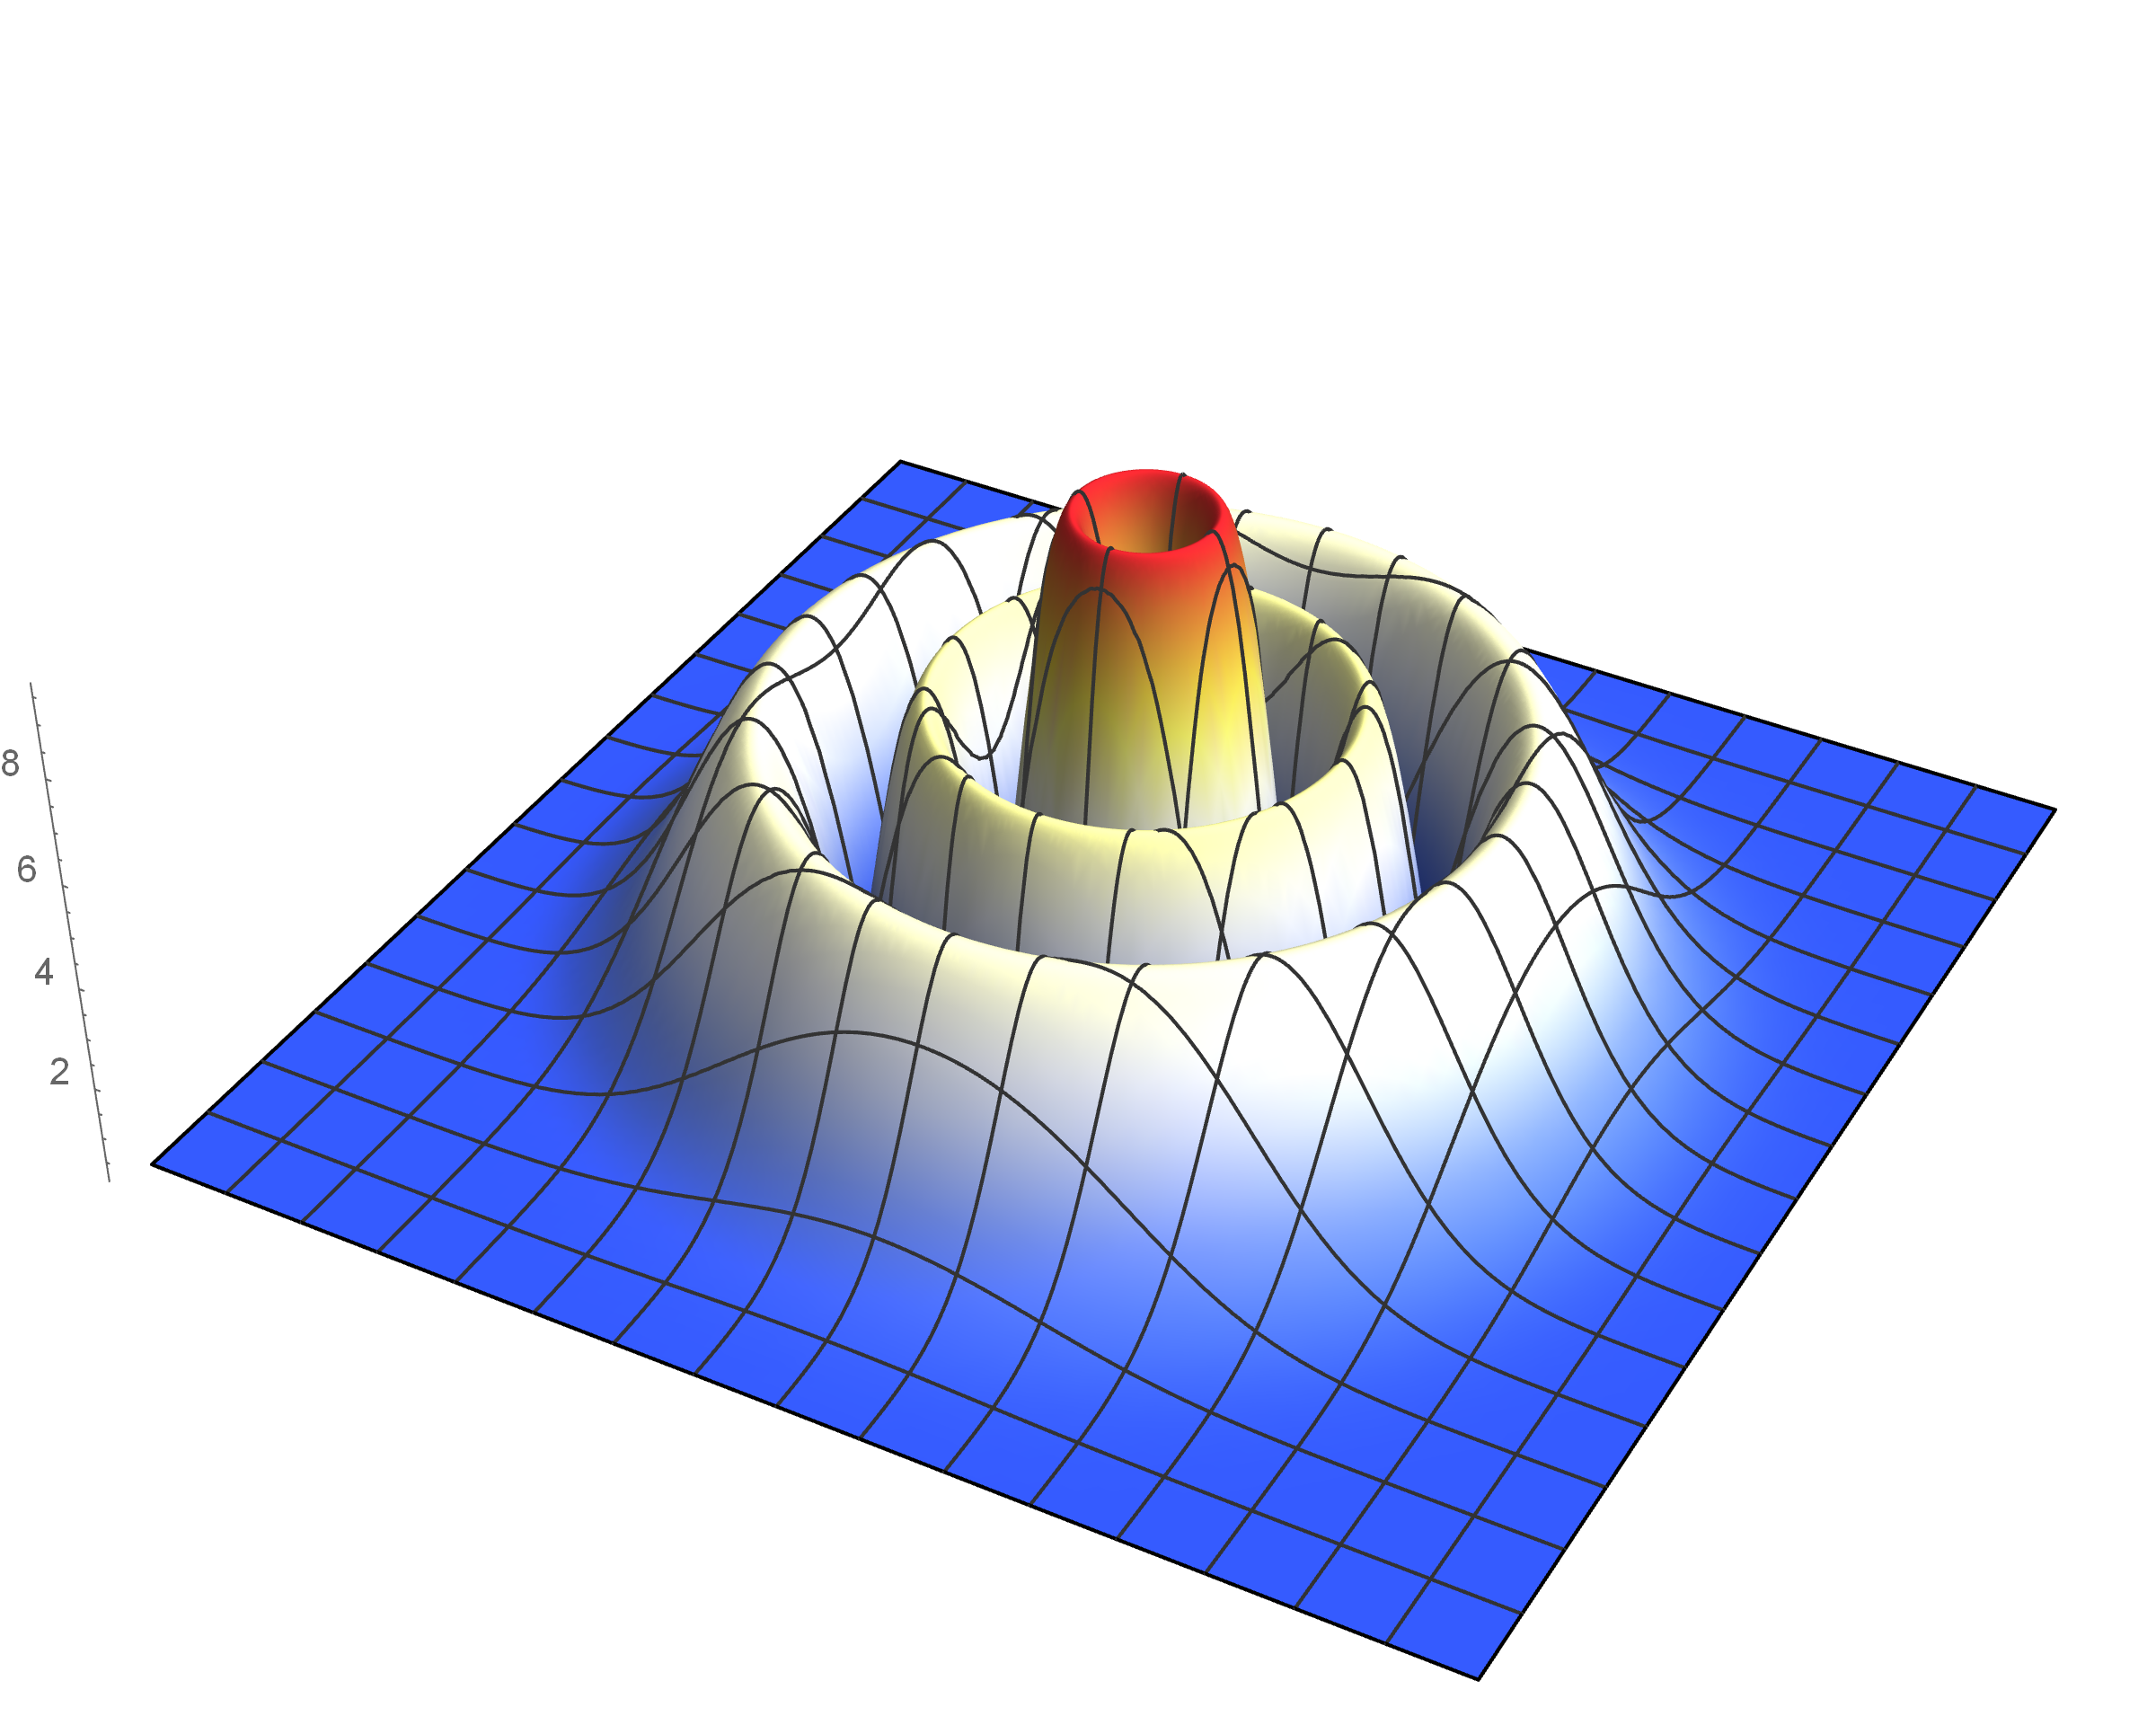
\includegraphics[width=1\textwidth]{Figures/OAM/LGBeamProfile_L1P2Z03.png} % second figure itself
        \caption{
        	Transverse profile of an OAM state with $\ell=1, p=2$.
        	% Transverse profile of an OAM state with $\ell=1, p=2, z=3$.
        }
        \label{fig:expQWs:LG_profile_L1P2Z03}
    \end{minipage}
\end{figure}

% % \FloatBarrier
% \section{State engineering protocol}
% \label{sec:expQWs:engineeringQWs}



\section{State engineering protocol}
\label{sec:expQWs:experimental_apparatus}

% \tmpHeading{What do we do?}
% In~\cref{sec:QWs:reachability_conditions,sec:QWs:focusing_walker_states} we showed that arbitrary qudits can be generated via suitable \ac{QW} dynamics. Here we present an experimental implementation of such protocol, showcasing its practicality in a few relevant scenarios.
% More specifically, we experimentally engineer six-dimensional qudits, focussing on a few physically relevant classes of states: \emph{angular-momentum Schrödinger cat states}, \emph{spin-coherent states}, completely balanced states, and randomly sampled states.

\tmpHeading{Our scheme to implement QWs}
We implement \acp{QW} with $n=5$ steps, using \ac{OAM} as the physical embodiment of the \emph{walker}, and the polarisation as the \emph{coin}. This allows the QW dynamics to take place in a single light beam.
% are encoded in circular-polarisation states $\{|R\rangle, |L\rangle\}$. We dub such degree of freedom as \ac{SAM} to mark the difference with \ac{OAM}.
The experimental setup, shown schematically in~\cref{fig:expQWs:schematics,fig:expQWs:proposal_exp}, is similar to the ones used in~\cite{cardano2015quantum,cardano2016statistical}.
The number of required optical elements scales linearly with the number of QW steps, thus avoiding the nonlinear growth of optical paths intrinsic to interferometric implementations~\cite{zhang2010implementation,goyal2013implementing}.
The coin operations are implemented by suitably arranging polarisation-rotating waveplates~\cite{simon1990minimal}. The shift operator is implemented using \acp{QP}~\cite{marrucci2006optical}. These are birefringent liquid-crystal devices that rise or lower the \ac{OAM} quantum number of impinging light conditionally to its polarisation ~\cite{marrucci2006optical}. More specifically, \acp{QP} act on \ac{OAM} states with azimuthal quantum number $m$ and polarisation $\ket L$ or $\ket R$ as follows:
\begin{equation}
\begin{aligned}
	\ket{L,m} & \xrightarrow{\text{QP}} \cos(\delta/2) \ket{L,m}
				+ i e^{\,-2 i \alpha_0}\, \sin(\delta/2) \ket{R,m+2q}, \\
	\ket{R,m} & \stackrel{\text{QP}}{\longrightarrow} \cos(\delta/2) \ket{R,m}
				+ i e^{-2 i \alpha_0} \sin(\delta/2) \ket{L,m-2q}.
\end{aligned}
\end{equation}
The parameter $q$ is referred to as the \emph{topological charge} of the device.
The phases $\alpha_0$ and $\delta$ are tunable by changing the orientation of the waveplates, and can be chosen so that the QP acts as
\begin{equation}
	\ket{R,m}\xrightarrow{\text{QP}} \ket{L,m-2q}
	\qquad\text{ and }\qquad
	\ket{L,m}\xrightarrow{\text{QP}}\ket{R,m+2q}.
\end{equation}
Single-photon states are generated via a type-II, collinear \ac{SPDC} source, separated with a \ac{PBS}, and then coupled to two \acp{SMF}. One photon acts as the trigger signal, while the other one undergoes the evolution.
% After propagation through the \ac{SMF} and the first \ac{PBS}, the state is $\ket{\psi_0}_{wc}=\ket{0}_w \otimes \ket{+}_c$ with $\ket{+}_c=(\ket{{\uparrow}}_c+\ket{{\downarrow}}_c)/\sqrt2$.
After the $5$ steps, the coin is projected onto $|+\rangle$, following the state engineering protocol outlines in~\cref{sec:QWs:focusing_walker_states}. This is experimentally implemented with a final \ac{PBS}.
To reconstruct the \ac{OAM} states thus generated, the light is coupled into a \ac{SMF} after passing through a \ac{SLM}. This allows to measure arbitrary \ac{OAM} states with high accuracy~\cite{bolduc2013exact,dambrosio2013test}.
The state fidelity between generated and target states is estimated by projecting the \ac{OAM} onto a basis containing the target state.

% Polarisation measurements are performed with waveplates and \acp{PBS}, while the \ac{OAM} is analysed with a \acp{SLM} and \acp{SMF}.
% The \ac{QW} is thus built out of a series of wave plates and QPs. The final state is projected onto OAM basis states using a \ac{SLM}, a \ac{SMF}, and an \ac{APD}.

\begin{figure}[tb]
\centering
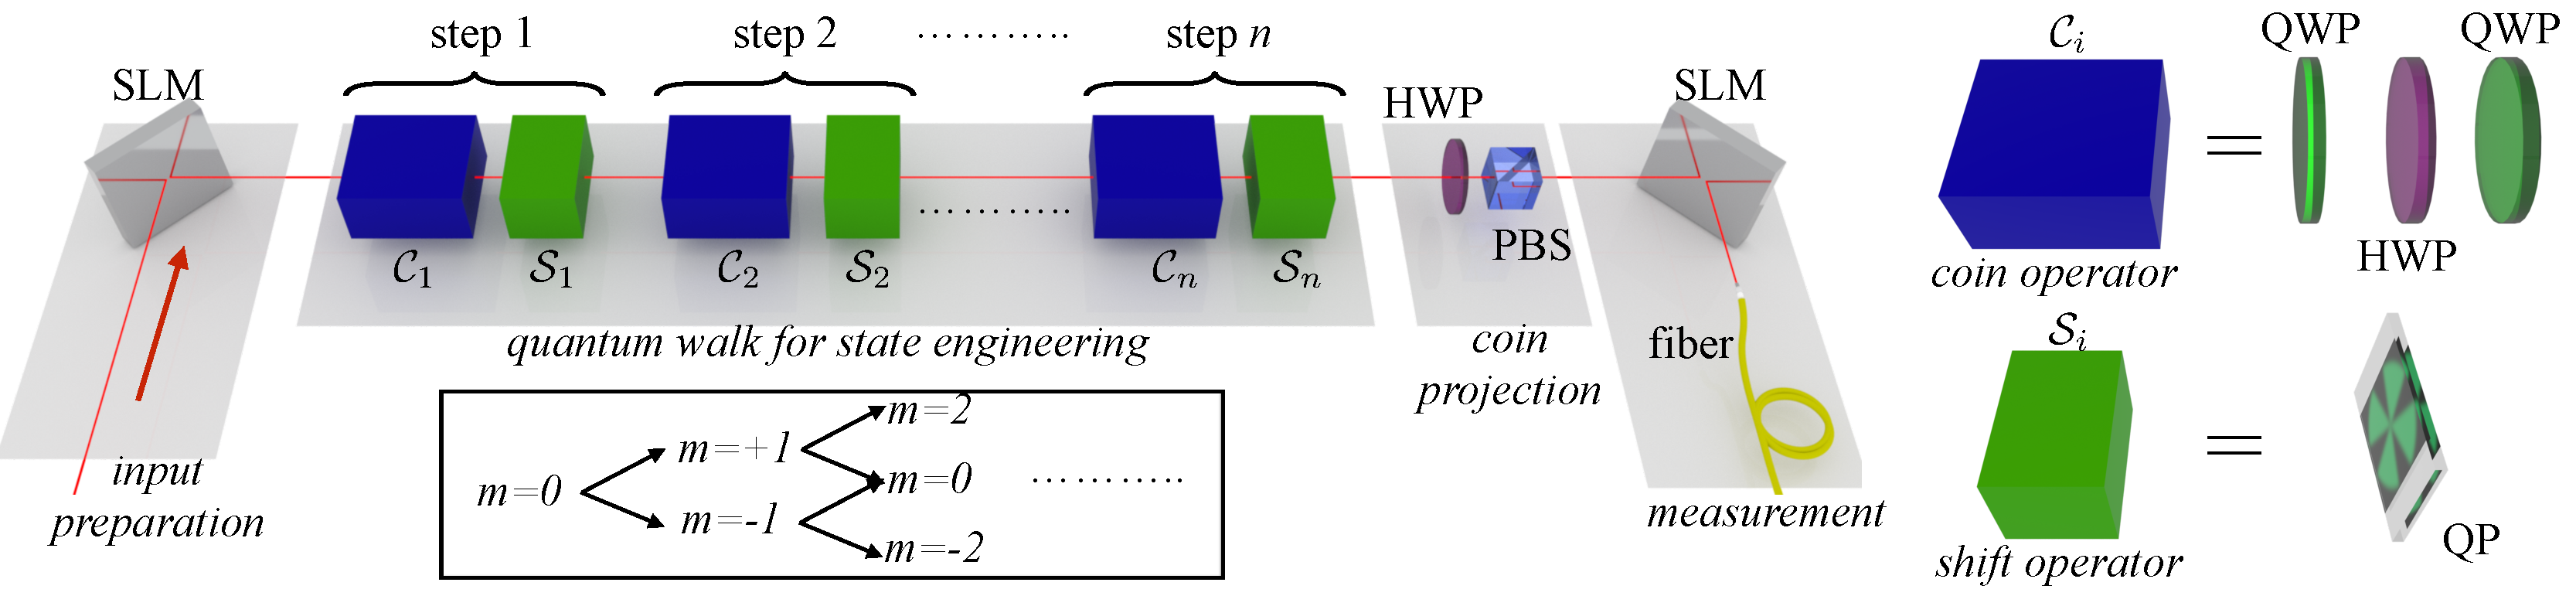
\includegraphics[width=0.99\textwidth]{experimental_apparatus_scheme.pdf}
\caption{
    Pictorial representation of the state engineering protocol.
    Input states are prepared using a \ac{SLM}.
    The coin operations are realised with sequences of \ac{QWP} and \ac{HWP}.
    The shift operations are implemented with \acp{QP}.
    The coin is projected at the end of the walk onto the state $\vert + \rangle$ using a \ac{HWP} and a \ac{PBS}.
    Finally, a \ac{SLM} and a \ac{SMF} are uesd to project the output states onto specific \ac{OAM} states.
}
\label{fig:expQWs:proposal_exp}
\end{figure}

\begin{figure}[tb]
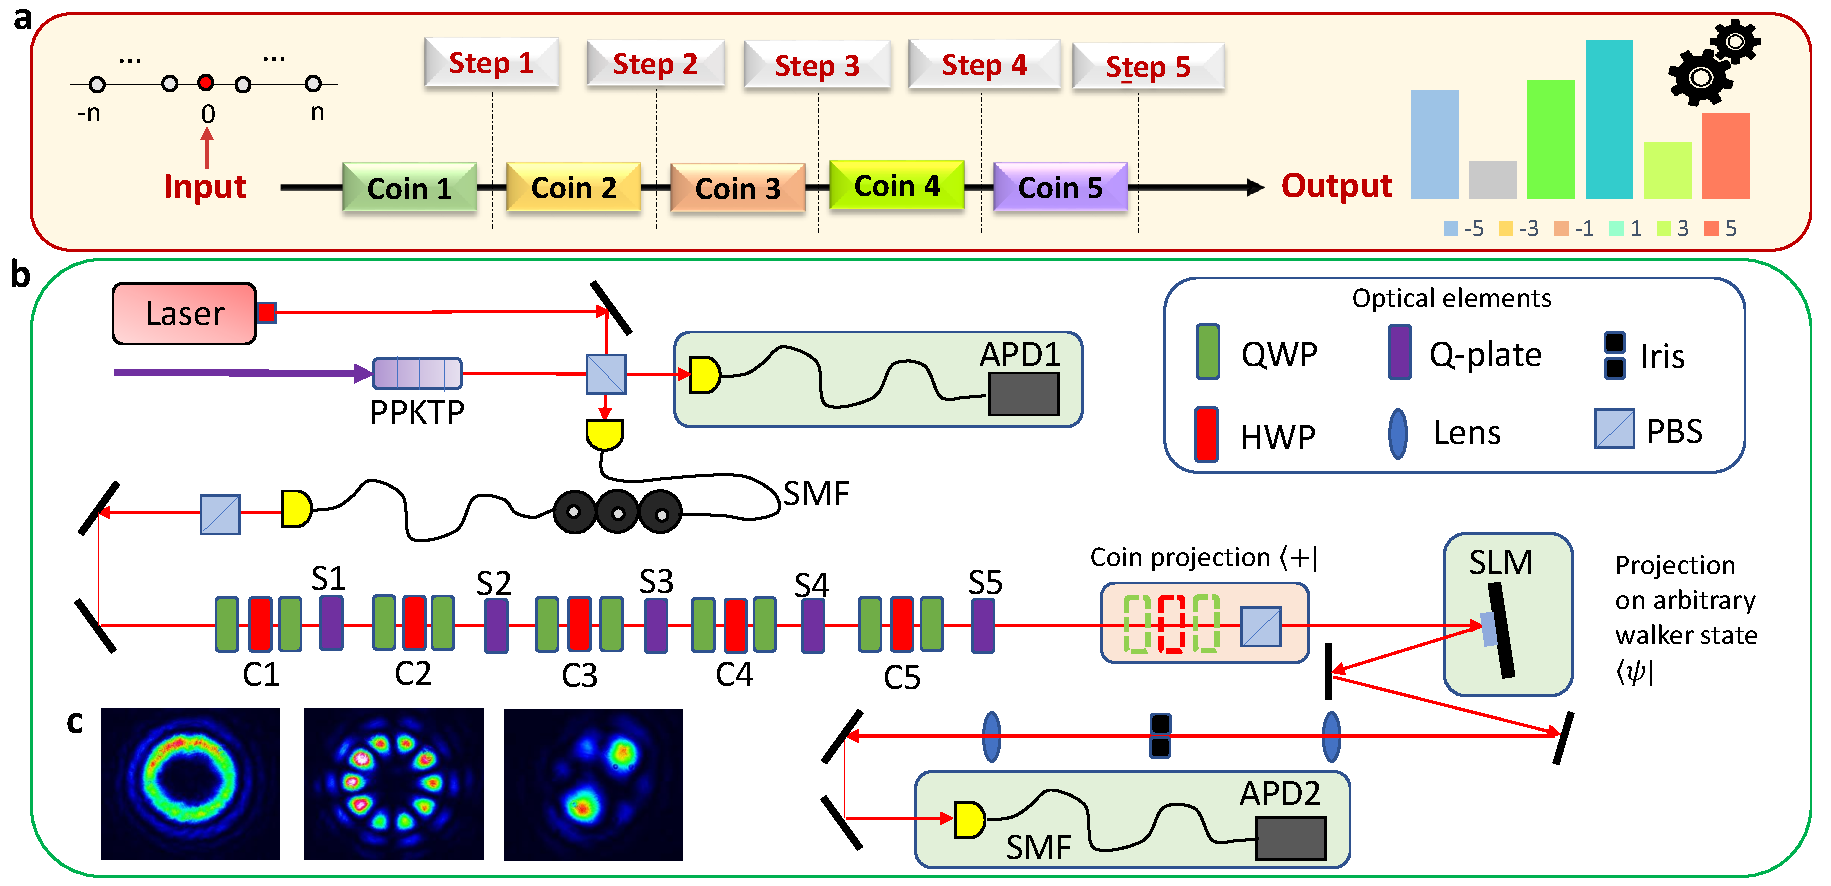
\includegraphics[width=\textwidth]{experimental-QSE-1.pdf}
\caption{
	More detailed representation of the quantum state engineering protocol also given in~\cref{fig:expQWs:proposal_exp}, with a focus on our specific implementation.
	\textbf{(a)} At each step the coin operator is changed to obtain a target state in the output.
	\textbf{(b)} A single-photon source, composed of a \ac{PPKTP} crystal, generates pairs of photons that are coupled in a SMF. One photon acts as trigger while the other is prepared in the state $\ket{+}\otimes \ket{0}$ through polarisation controllers and a \ac{PBS}. Five sets of \acp{QWP} and \acp{HWP} implement the coin operators at each step. Five \acp{QP} implement the shift operation after each coin operation.
	The detection stage consists of a \ac{PBS} followed by a \ac{SLM}, a \ac{SMF} and an \ac{APD}.
	\textbf{(c)} Pictures of \ac{OAM} modes detected after the \ac{PBS}, obtained using coherent light. From right to left: \ac{OAM} eigenstate corresponding to $m=5$; balanced superposition of $m=\pm 5$; balanced superposition of all \ac{OAM} components covered by 5-step \ac{QW} $m=\{\pm 5, \pm 3, \pm 1\}$.
}
\label{fig:expQWs:schematics}
\end{figure}

\tmpHeading{Coupling light into the QPs}
Experimental limitations in the maximum achievable number of steps are due to the generation process of \ac{OAM} eigenstates by the \acp{QP}. To prevent coupling between the radial and azimuthal parts of the beam during the propagation in free space, all of the evolution has to happen in the near-field regime~\cite{karimi2009light,cardano2015quantum}. This means that the distance $\ell$ between consecutive \acp{QP} has to be such that $\xi\equiv \ell/z_R \ll 1 $, where $z_R$ is the Rayleigh range.
In our setup, the beam waist $w_0$  ensures a $z_R> \SI{30}{\meter}$ at wavelength $\lambda=\SI{808}{nm}$. Two adjacent \acp{QP} are separated by a distance $\ell \sim \SI{15}{cm}$ (this distance is needed to insert, between the \acp{QP}, the waveplates implementing the coin), such that the condition on $\xi$ is satisfied.  Furthermore, in this regime the Gouy phase can be neglected allowing a good control of the coherence between different \ac{OAM} components, and, consequently, on the output states. However, in the perspective of implementing a higher number of steps, the requirement to have a $z_R$ large at least as the total length $L$ of the platform also implies a large beam waist, thus limiting the maximum amount of steps that can be implemented. An alternative strategy could be to use a loop scheme, where consecutive steps are performed by multiple passes through the same \ac{QP} and waveplates~\cite{goyal2013implementing}. In this alternative setup, a suitable $4f$ lens system is necessary to image the output of the QP to the input of the next step, being such approach equivalent to work in the near-field regime.  
In this combined \ac{OAM}-loop scheme, experimental challenges arise at the measurement stage, that in spin-\ac{OAM} setup involves a \ac{SLM}. When integrating such encoding in a loop-architecture, issues may arise due to their slow response time.


\section{Results}
\label{sec:expQWs:results}

\tmpHeading{Types of generated states}
To demonstrate the flexibility of the protocol, we showcase the generation of a variety of states, including
% \begin{enumerate}
% 	\item Computational basis states;
% 	\item Cat-like states (see~\cref{subsec:expQWs:catstates});
% 	\item \acp{SCS} (see~\cref{subsec:expQWs:SCSs});
% 	\item Completely balanced and randomly sampled states;
% 	\item Fourier basis states.
% \end{enumerate}
computational basis states, completely balanced states, random states, Fourier basis states, cat-like states (see~\cref{subsec:expQWs:catstates}), and \acp{SCS} (see~\cref{subsec:expQWs:SCSs}).
% We start by generating the elements of the computational basis corresponding to the eigenstates of the \ac{OAM}: $\{\ket{m} \}=\{\ket{\pm5}, \ket{\pm3},\ket{\pm1} \}$. We then generate superpositions of two computational basis states, and then proceed with more complex states such as spin-coherent states, the elements of the Fourier basis, and lastly random states.
% The quantum state fidelities are calculated projecting onto the elements of an orthonormal basis containing the target state.
\Cref{table:expQWs:summary} contains a summary of the states engineered with the corresponding fidelities and generation probabilities,
while~\cref{table:expQWs:random_states_amps} gives the explicitly the random target states we used.
In~\cref{fig:expQWs:results_cat_states,fig:VVBs:results_SCS_states} we give the experimental results for the generation of cat-like states and \acp{SCS}, respectively.
The fidelity between experimentally synthesised and target states is computed by projecting the state onto an orthonormal basis which contains the target state.
% In~\cref{fig:VVBs:results_SCS_states}\textbf{f}, we report the fidelities for all the experimentally engineered states.
% The red area shows the average fidelity and its uncertainty ($\mathcal{F}{=}0.954 \pm 0.001$). Such test provides further evidence of the effectiveness of our engineering strategy.

\tmpHeading{Scaling of projection probabilities}
% As mentioned in~\cref{sec:QWs:focusing_walker_states}, multiple \ac{QW} dynamics can, after projection of the coin, lead to the same target state.
% These different solutions will in general correspond to different projection probabilities.
% To find the coin operators leading to each target state we used the numerical optimisation method presented in~\cref{sec:QWs:numerical_fid_max}.
% To assess the average scaling on the projection probability, we simulated QWs of up to $20$ steps using the algorithm of~\cref{sec:QWs:numerical_fid_max} to find coin operations generating different target states. We found the projection probabilities to have a roughly linear scaling, and remain $\ge 15\%$ for up to $20$ steps of our protocol, as shown in~\cref{fig:expQWs:avgProbabilitiesVsStepNumber}.
In~\cref{fig:expQWs:avgProbabilitiesVsStepNumber} we show the \textit{average} projection probability as a function of the number of steps. These probabilities are calculated by averaging the projection probabilities obtained by running the optimisation algorithm given in~\cref{sec:QWs:numerical_fid_max} over many uniformly sampled random states, for various numbers of steps. We find the average projection probability to decrease roughly linearly with the number of steps. If we assume this linear decrease to also hold for larger numbers of steps, the average projection probability would be dropping to $\sim 0.1$ at around $25$ steps, and remains $\ge 0.15$ for up to $20$ steps.
We note that this likely underestimates the actual probabilities. Indeed, as already mentioned, this optimisation method finds only one among many solutions for a given target, and thus generally not the optimal one in terms of projection probability. Moreover, increasing the step number also increases the number of paths with which a state can be generated, which means that, with this method, we can expect the underestimation to be even more significant for larger step numbers.
Further evidence suggesting that this method underestimates the real average probabilities is obtained by computing the full set of solutions and taking the optimal one, which can be done for up to five steps. Indeed, as shown in~\cref{sec:QWs:numerical_fid_max}, with this method we find the real optimal average probabilities for three, four, and five steps to be consistently $\sim 0.33$, with no detectable decreasing behaviour.

\begin{table}[tbh]
\centering\footnotesize
\begin{tabular}{lcc|lcc}
\toprule
Target State & Probability  & Fidelity & Target State & Probability  & Fidelity \\
\midrule
 $\quad\ket{-5}$ & $0.5$  & $0.981 \pm 0.007\quad$ & $\quad\ket{\on{QFT}_1}$ & $0.14$ & $0.969\pm 0.007$\\
 $\quad\ket{-3}$ & $0.5$ & $0.982 \pm 0.007\quad$ & $\quad\ket{\on{QFT}_2}$ & $0.17$ & $0.923\pm 0.022$ \\
 $\quad\ket{-1}$ & $0.5$ & $0.960 \pm 0.007\quad$ & $\quad\ket{\on{QFT}_3}$ & $0.17$ & $0.911\pm 0.011$\\ 
 $\quad\ket{1}$ & $0.5$ & $0.995 \pm 0.007\quad$ & $\quad\ket{\on{QFT}_4}$&$0.17$ &  $0.980\pm 0.011$ \\
 $\quad\ket{3}$ & $0.5$ & $0.975 \pm 0.007\quad$ & $\quad\ket{\on{QFT}_5 }$& $0.17$& $0.936\pm 0.011$ \\
 $\quad\ket{5}$ & $0.5$ & $0.994 \pm 0.001\quad$ & $\quad\ket{\on{QFT}_6} $& $0.17$ & $0.945\pm 0.007$ \\
 $\quad\frac{1}{\sqrt{2}}\left(\ket{-5}+\ket{5} \right)$ & $0.5$  & $0.995 \pm 0.001\quad$ &$\quad\ket{r_1}$ & 0.22& $0.911\pm0.011$\\
 $\quad\frac{1}{\sqrt{2}}\left(\ket{-5}-\ket{5}\right)$ & $0.5$ & $0.947 \pm 0.002\quad$ &$\quad\ket{r_2}$  & 0.16 & $0.923 \pm 0.012$\\
 $\quad\frac{1}{\sqrt{2}}\left(\ket{-5}+i\ket{5}\right)$ & $0.5$ & $0.969 \pm 0.002\quad$ &$\quad\ket{r_3}$  & 0.17 & $0.941 \pm 0.004$\\ 
  $\quad\frac{1}{\sqrt{2}}\left(\ket{-5}-i\ket{5}\right)$ & $0.5$ & $0.936 \pm 0.003\quad$&$\quad\ket{r_4} $& 0.14 &$0.947 \pm 0.015$  \\
 %$\frac{1}{\sqrt{2}}\left(\ket{-3}+\ket{3}\right)$ & $0.5$ & $0.912 \pm 0.004$ \\
 $\quad\ket{S_1}=\ket{5/2,\pi /2,0}$ & $0.15$ & $0.970 \pm 0.002\quad$ &$\quad\ket{r_5}$ & 0.19 & $0.950\pm0.005$  \\
 $\quad\ket{S_2}=\ket{5/2,-\pi /2,0}$ & $0.15$ & $0.961 \pm 0.003\quad$ &$\quad\ket{c_1}$ &0.16 & $0.956\pm0.004$ \\
 $\quad\frac{1}{\sqrt{2}}\left(\ket{S_1}+\ket{S_2}\right)$ & $0.15$ & $0.932 \pm 0.004\quad$&$\quad\ket{c_2}$ & 0.29 &$0.935 \pm 0.006$  \\
 $\quad\frac{1}{\sqrt{2}}\left(\ket{S_1}-\ket{S_2}\right)$ & $0.15$ & $0.942 \pm 0.004\quad$& $\quad\ket{c_3}$& 0.17 & $0.925\pm 0.008$ \\
$\quad\frac{1}{\sqrt{2}}\left(\ket{S_1}-i\ket{S_2}\right)$ & $0.23$ & $0.974 \pm 0.003\quad$&$\quad\ket{c_4}$ & 0.16 & $0.944\pm0.008$\\
$\quad\frac{1}{\sqrt{2}}\left(\ket{S_1}+i\ket{S_2}\right)$ & $0.23$ & $0.964 \pm 0.004\quad$& $\quad\ket{c_5}$ & 0.28 & $0.946\pm0.004$\\
\bottomrule
\end{tabular}
\caption{%
	Generated states with associated projection probabilities and fidelities.
	Left column: computational basis states $\ket k$ with $k\in\{-5,-3,-1,1,3,5\}$, cat-like states, and \acp{SCS} $\ket{S_i}$ and their superpositions.
	Right column: Fourier basis states $\ket{\on{QFT}_k}$, random real states $\ket{r_k}$, and random complex states $\ket{c_k}$.
	The Fourier basis states are defined as $\ket{\on{QFT}_k}=\frac{1}{\sqrt{6}}\sum_{j=1}^{6}e^{\frac{ i \pi jk }{3}}\ket{j}$.
}
\label{table:expQWs:summary}
\end{table}

\begin{table}[tbh]
\centering\footnotesize
\begin{tabular}{cc}
\toprule
State & Amplitudes \\
\midrule
$\qquad\ket{r_1}\qquad$& $\left( 0.51, 0.27, 0.13, 0.10, 0.29, 0.75\right)$\\
$\qquad\ket{r_2}\qquad$& $\left( 0.19, 0.40, 0.04, 0.53, 0.37, 0.62\right)$\\
$\qquad\ket{r_3}\qquad$&$\left( 0.50, 0.74, 0.40, 0.16, 0.10, 0.006\right)$ \\
$\qquad\ket{r_4}\qquad$& $\left( 0.50, 0.47, 0.55, 0.31, 0.36, 0.04\right)$ \\
$\qquad\ket{r_5}\qquad$& $\left( 0.24, 0.12, 0.72, 0.16, 0.54, 0.30\right)$ \\
$\qquad\ket{c_1}\qquad$& $\left( 0.04+0.35i, 0.34+0.41i, 0.10+0.42i, 0.18-0.26i, 0.11-0.11i, -0.47+0.22i\right)$  \\
$\qquad\ket{c_2}\qquad$& $\left( 0.19-0.33i, -0.43+0.30i, -0.18-0.02i, -0.37+0.42i, -0.12-0.10i, 0.23+0.38i\right)$\\
$\qquad\ket{c_3}\qquad$& $\left( -0.19-0.30i, -0.02+0.39i, 0.30-0.15i, 0.25-0.22i, -0.13+0.42i, 0.24+0.48i\right)$\\
$\qquad\ket{c_4}\qquad$& $\left( 0.06+0.07i, 0.30-0.37i, -0.23+0.08i, 0.11-0.13i, -0.22+0.57i, 0.07-0.54i\right)$\\
$\qquad\ket{c_5}\qquad$& $\left( 0.07+0.14i, 0.48-0.34i, -0.41-0.18i, -0.41-0.09i, -0.10+0.32i, 0.32+0.18i\right)$\\
\bottomrule
\end{tabular}
\caption{
	Amplitudes of the random target states.
	The real states $\ket{r_k}$ have been sampled uniformly in the range $\left[0,1\right]$ and then normalised. In the case of complex states we have sampled the real and imaginary part separately in the range $\left[-0.5,0.5\right]$.
}
\label{table:expQWs:random_states_amps}
\end{table}

\subsection{Cat-like states}
\label{subsec:expQWs:catstates}

\tmpHeading{What do we mean by ``cat-like states''}
\emph{Schrödinger's cat states} are quantum superpositions of macroscopically distinct states~\cite{yurke1986generating,bužek1995quantum}.
These states play an important role in the investigations of the foundations of quantum mechanics~\cite{schrodinger1935gegenwartige} and their generation is at the core of various quantum engineering protocols~\cite{brune1992manipulation, monroe1996schrodinger,agarwal1997atomic, zhang2016creating}.
In the context of QWs, we define \emph{cat-like states} as coherent superpositions of two extremal sites of the walker, that is, in our case, states of the form $\alpha\ket{5}+\beta\ket{-5}$~\cite{zhang2016creating}. The isomorphism between \ac{OAM} with an angular momentum of quantum number $n/2$ allows to put in correspondence the position states $\ket{\pm 5}$ of the walker with angular momentum states with minimum and maximum projections onto the quantisation axis $\ket{\pm 5/2}$ (for simplicity of notation, we will use position states only). Such isomorphism makes a coherent superposition state such as $(\ket{5}+e^{i\varphi}\ket{-5})/\sqrt{2}$ (with $\varphi$ a suitable phase) into a faithful angular momentum SCS~\cite{militello2006distilling}. 
% Experimental generation of cat-like states has been previously reported in atomic systems~\cite{leibfried2005creation}.


\begin{figure}[tb]
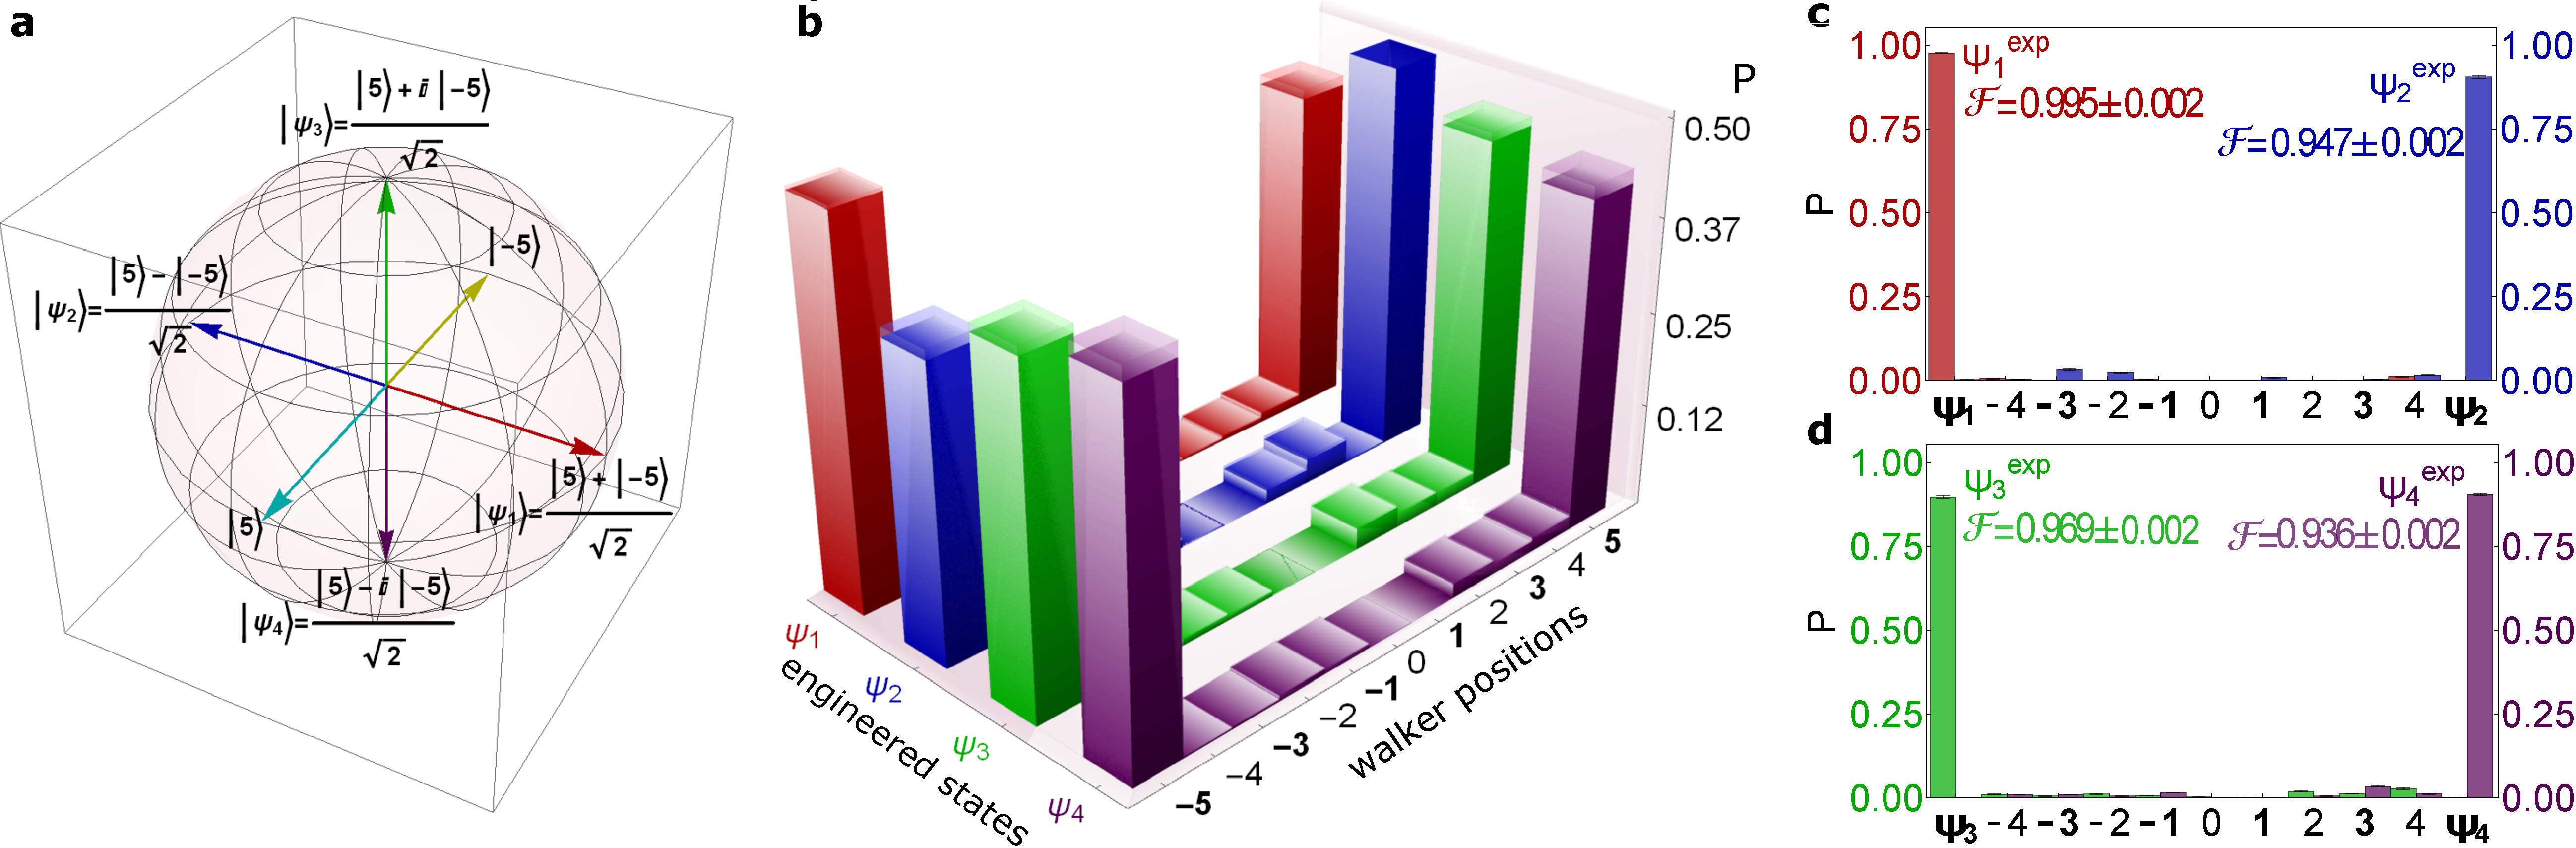
\includegraphics[width=\textwidth]{experimental-QSE-2.pdf}
\caption{
	Experimental results for the engineering of angular momentum cat states.
	\textbf{(a)} Representation on a Bloch-like ball of the four target states corresponding to the superposition of $\ket{\pm 5}$, which correspond corresponding to \ac{OAM} states with maximum and minimum projection of the angular momentum along the quantisation axis.
	\textbf{(b)} Population of the \ac{OAM} components after 5-step {QW} for the states $\ket{\psi_i}~(i=1,2,3,4)$ in panel {\bf a}. Odd-$m$ position states (bold numbers on $x$-axis) should be the only ones involved in the state engineering. However, we report also the populations of even-$m$ position states (light-black numbers on $x$-axis) to illustrate possible imperfections at generation and detection stages. The error bars associated with experimental populations are shown by the transparent areas on top of each histogram.
	\textbf{(c)-(d)} Distributions of probabilities $P_i=\langle B^{(j)}_i\vert\rho_\text{exp}\vert B^{(j)}_i\rangle~(j=1,2)$ that the experimental walker state $\rho_\text{exp}$ is found to be one of the elements of the bases $B^{(j)}=\{\ket{\psi_p},\ket{\psi_{p+1}},\ket{\pm4},\ket{\pm3},\ket{\pm2},\ket{\pm1},\ket{0}\}$ with $p=1$ for $j=1$ and $p=3$ for $j=2$. All the error bars are due to Poissonian uncertainties, propagated through Monte Carlo methods. The state fidelities ${\cal F}$ are calculated as described in the main text.
}
\label{fig:expQWs:results_cat_states}
\end{figure}

\begin{figure}[tb]
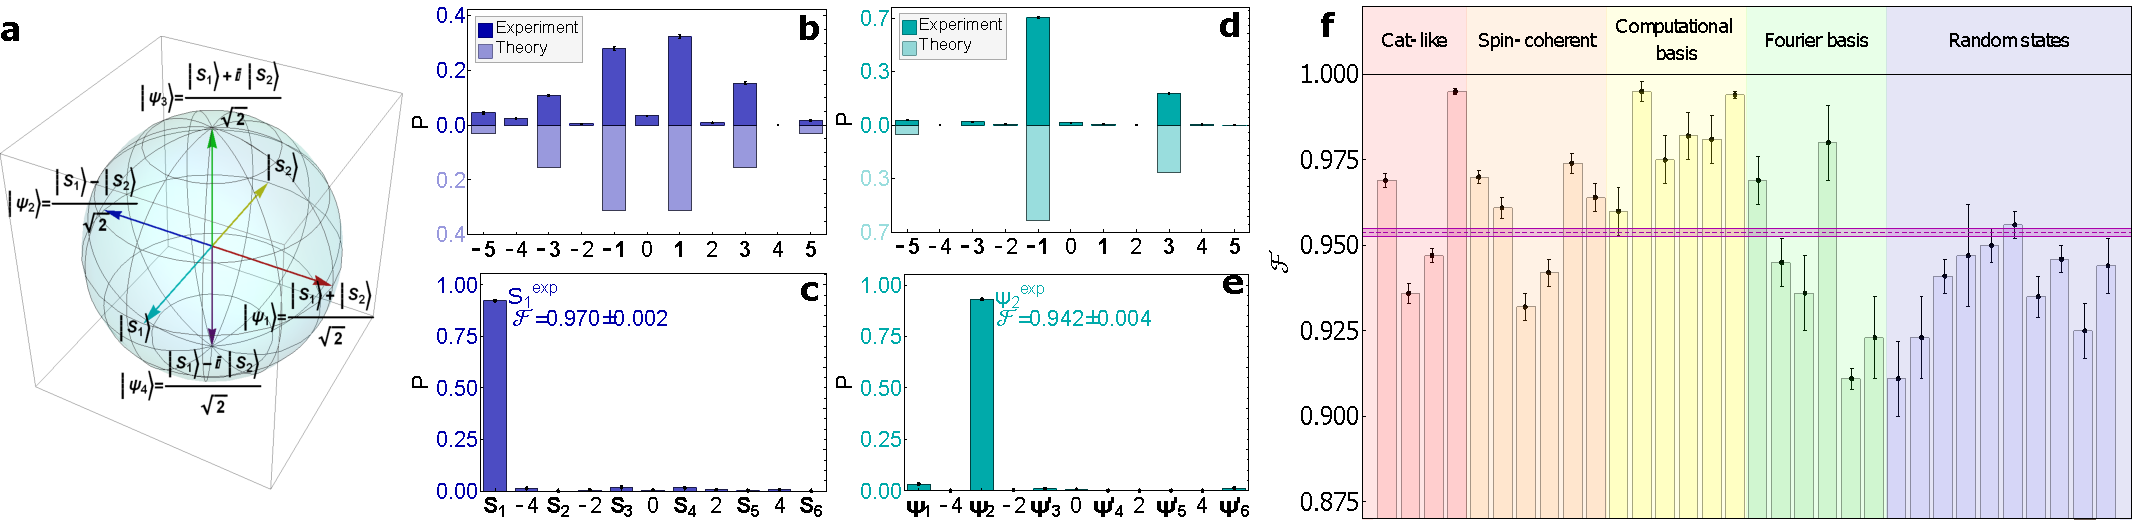
\includegraphics[width=\textwidth]{experimental-QSE-3.pdf}
\caption{
	Experimental results for the engineering of \acp{SCS} and their coherent superposition:
	\textbf{(a)} Bloch-sphere representation for the mutually orthogonal \acp{SCS} $\ket{S_1}$ and $\ket{S_2}$.
	\textbf{(b)} Probability distributions associated to the projection of $\ket{S_1}$ onto the computational basis. As previously explained, we also consider the contribution of even \ac{OAM} components.
	\textbf{(c)} Probability distribution corresponding to the basis that contains the target state itself $\ket{S_1}$, generated with the fidelity reported in the panel. Such orthonormal basis, $\{S_i\}_i$ with $i=1 ...6$, contains eigenstates of $\hat{S}_x$ for a particle with spin $s=5/2$ that are in turn all spin-coherent states.
	\textbf{(d)} Experimental probability distribution on computational basis for $\ket{\psi_2}=\frac{1}{\sqrt{2}}\left(\ket{S_1}- \ket{S_2} \right)$. Only components $\{-5, -1, 3\}$, corresponding to logical states $\{1,3,5\}$, have non-zero probabilities.
	\textbf{(e)} Quantum state fidelity evaluated measuring state $\ket{\psi_2}$ on the orthonormal basis that contains state $\ket{\psi_1}$, as described in the main text. 
	\textbf{(f)} Summary of quantum state fidelities for the $32$ states generated in the experiment. The average fidelity, $\bar{\calF}=0.954\pm 0.001$, is reported by the magenta area.
}
\label{fig:VVBs:results_SCS_states}
\end{figure}

\begin{figure}[tb]
    \centering
    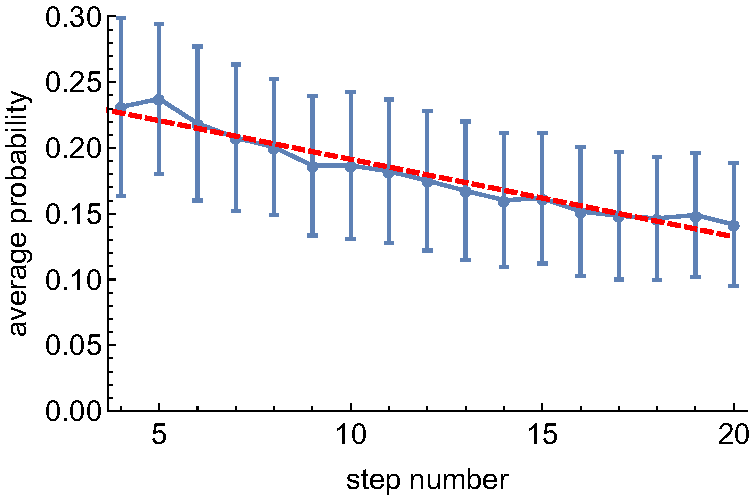
\includegraphics[width=0.8\linewidth]{experimentalQSE-averagesAndVariances_rerundata_manysteps.pdf}
    \caption{
    	Average projection probability obtained for randomly sampled target states with different numbers of steps. Each point corresponds to an average over a sample of $2000$ uniformly sampled random target states of the given dimension. For each target, an optimisation algorithm is used to find a solution producing it, as discussed in~\cref{sec:QWs:numerical_fid_max}. The error bars represent the standard deviation associated with each point. The red dashed line is a linear fit. It should be noted that, as discussed in~\cref{sec:QWs:numerical_fid_max}, this data provides only a lower bound to the real average probabilities.%
    }
    \label{fig:expQWs:avgProbabilitiesVsStepNumber}
\end{figure}

\subsection{Spin-coherent states}
\label{subsec:expQWs:SCSs}

% The second class of states that we consider are \emph{spin-coherent states}~\cite{ulyanov1999spin}, which are the spin-like counterpart of \emph{coherent states} of a quantum harmonic oscillator.

\tmpHeading{What are SCSs?}
\acfp{SCS} are the counterparts of coherent states of the harmonic oscillator for a particle with spin $s$~\cite{radcliffe1971some,arecchi1972atomic,agarwal1997atomic,markham2003classicality,chryssomalakos2018geometry}. They are the eigenstates, with eigenvalue $s$, of $S_{\theta,\phi}$, the component of the total spin-momentum operator along the direction identified by the spherical angles $(\theta, \phi)$~\cite{arecchi1972atomic,agarwal1997atomic,ulyanov1999spin,lee2015visualizing}.
A decomposition of such states over the $\{\ket{m}\}$ basis of the projected spin along the $z$-direction, $S_z$, reads
\begin{equation}
\begin{aligned}
	\ket{s,\theta,\phi} &=
		\sum_{m=-s}^{s}
		\sqrt{\frac{(2s)!}{(s+m)!(s-m)!}} e^{-i\phi m} C_\theta^{s+m} S_\theta^{s-m}\ket{m},
\end{aligned}
\label{spin_coherent1}
\end{equation}
with $C_\theta\equiv\sqrt{1-S^2_\theta}=\cos(\theta/2)$. \acp{SCS} have numerous applications in condensed matter physics, in particular for quasi-exactly solvable models, for the Wigner-Kirkwood expansion and in quantum correction to energy quantisation rules~\cite{ulyanov1999spin}. At a more foundational level, they can be used to generate Schrödinger cat states~~\cite{agarwal1997atomic}. 


Although \acp{SCS} are in general not orthogonal, they form a convenient basis. Moreover, as two \acp{SCS} pointing in opposite azimuthal directions are orthogonal for $\theta\sim\pi/2$, by restricting the attention to $\{\ket{s,\pi/2,\phi},\ket{s,-\pi/2,\phi}\}$ we would be dealing with an orthonormal basis, which we can use to construct the analogous of a Bloch ball for a two-level system (cf.~\cref{fig:VVBs:results_SCS_states}\textbf{a}). We have thus engineered $\ket{S_1}\equiv\ket{5/2,\pi/2,0}$ and $\ket{S_2}\equiv\ket{5/2,-\pi/2,0}$, and considered the experimental synthesis of balanced coherent superpositions of such states.
Furthermore, $S_1$ and $S_2$ are also eigenstates of the $\hat{S}_x$ operator. In~\cref{fig:VVBs:results_SCS_states}\textbf{b-c} the state $S_1$ is projected firstly on the computational basis, the eigenstates of $\hat{S_z}$, and then on the basis $\{S_i\}$, with $i=1...6$, which consists of $\hat{S}_x$ eigenstates. Balanced superpositions of $S_1$ and $S_2$ are akin to the Schrödinger cat states built on coherent states of a harmonic oscillator, as they exhibit signatures of non-classical interference~\cite{agarwal1997atomic}. For instance, only even (odd) components of the logical basis enter the superpositions $\ket{S_1}\pm\ket{S_2}$, a parity rule that is fully analogous to the one characterising even (odd) bosonic cat states. Thanks to the isomorphism between the spaces of \ac{OAM} and of arbitrary angular momentum equal to $n/2$, we can generate \ac{SCS} mapping the basis $\{ \ket{s_z}\}$ in~\cref{spin_coherent1} into the basis of the \ac{QW} $\{|m\rangle\}$. The results are illustrated in~\cref{fig:VVBs:results_SCS_states}\textbf{a-e}, where we show the high quality of both the generated \acp{SCS}and \ac{SCS}-based cat states.

\subsubsection{Cat states based on spin coherent states: phase-space picture}
\highlight{Riarrangiare}

The decomposition of a \ac{SCS} $\ket{s,\theta,\phi}$ over the basis of eigenstates of angular momentum $\{\ket{m}\}_{m=-s}^s$ reads
\begin{equation}
	\ket{s,\theta,\phi} =
	\sum^s_{m=-s}
		\sqrt{\frac{(2s)!}{(s+m)!(s-m)!}}
		e^{-i\phi m} C^{s+m}_\theta S^{s-m}_\theta \ket{m},
\end{equation}
with $C_\theta\equiv\sqrt{1-S^2_\theta}=\cos(\theta/2)$. We have also introduced the \ac{SCS}-based Schrödinger cat states built as the following superpositions of orthogonal states $\ket{S_1}:=\ket{5/2,\pi/2,0}$ and $\ket{S_2}:=\ket{5/2,-\pi/2,0}$:
\begin{equation}
%\begin{aligned}
\ket{\psi_{1}}=\frac{1}{\sqrt 2}(\ket{S_1}+\ket{S_2}),\qquad\ket{\psi_{2}}=\frac{1}{\sqrt 2}(\ket{S_1}-\ket{S_2}).
%\end{aligned}
\end{equation}
In this Section, we aim at providing a brief analysis of the features of such states, which are best analyzed in a suitably defined phase space~\cite{agarwal1997atomic}. In particular, we shall be considering the analogous of the Husimi $Q$ function~\cite{walls2007quantum} defined as
\begin{equation}
\label{deco}
Q_j(\alpha,\beta)=\vert\langle{5/2,\alpha,\beta}\vert\psi_j\rangle\vert^2\qquad(j=1,2)
\end{equation}
in the spherical polar space where the Cartesian coordinates $(x,y,z)$ are mapped into $x\to Q_j(\alpha,\beta)\sin\alpha\cos\beta$, $y\to Q_j(\alpha,\beta)\sin\alpha\sin\beta$ and $z\to Q_j(\alpha,\beta)\cos\alpha$. Despite the simplicity of its definition, $Q_j(\alpha,\beta)$ captures important information about the quantum interference between the orthogonal components of $\ket{\psi_{j}}$, which differentiate such states from the incoherent mixture of \acp{SCS} $(\ket{S_1}\bra{S_1}\pm\ket{S_2}\bra{S_2})/2$. 

The orthogonality of $\ket{S_1}$ and $\ket{S_2}$ allows one to cast $Q_j(\alpha,\beta)$ as 
\begin{equation}
Q_j(\alpha,\beta)=\frac12\left(|q_+(5/2,\alpha,\beta)|^2+|q_-(5/2,\alpha,\beta)|^2+\text{sign}_j2\text{Re}[q_+(5/2,\alpha,\beta)q^*_-(5/2,\alpha,\beta)]\right)
\end{equation}
where $q_\pm(s,\alpha,\beta)=\bra{s,\alpha,\beta}{s,\pm\theta,0}\rangle$ and $\text{sign}_1=-\text{sign}_2=+1$. Such scalar products can be evaluated explicitly for any value of $s$ by using the decomposition in Eq.~\eqref{deco} to get 
\begin{equation}
\begin{aligned}
q_\pm(\alpha,\beta)&=(\pm 1)^s\frac{\Gamma (2 s+1)}{\Gamma (s+1)^2} S^s\left({\alpha }\right) C^s\left(\alpha\right) S^s\left(\theta\right) C^s\left({\theta
   }\right) \left[\, _2F_1\left(1,-s;s+1;\mp e^{-i \beta  } T\left({\alpha}\right) T\left({\theta }\right)\right)\right.\\
  &+\left.{}_2F_1\left(1,-s;s+1;\mp e^{i \beta} T^{-1} \left({\alpha}\right) T^{-1}\left({\theta }\right)\right)-1\right],
  \end{aligned}
\end{equation}
where $T(\alpha)=S(\alpha)/C(\alpha)=\tan(\alpha/2)$, $_2F_1(a,b,c;d)$ is the ordinary Hypergeometric function, and $\Gamma(d)$ is the Gamma function with argument $d$.

Using such expressions, we can compute $Q_j(\alpha,\beta)$ to investigate its features. However, looking at such function directly does not provide sufficient information for the discrimination of an incoherent mixture and a state such as $\ket{\psi-{1,2}}$. On the other hand, we find more informative to consider that $\frac12\left(|q_+(5/2,\alpha,\beta)|^2+|q_-(5/2,\alpha,\beta)|^2\right)$ is precisely the spherical SCS-based $Q$ function for the incoherent state $(\ket{S_1}\bra{S_1}\pm\ket{S_2}\bra{S_2})/2$. Let us call it $Q_{inc}(\alpha,\beta)$, so that 
\begin{equation}
Q_j(\alpha,\beta)=Q_{inc}(\alpha,\beta)+\text{sign}_j\text{Re}[q_+(5/2,\alpha,\beta)q^*_-(5/2,\alpha,\beta)],
\end{equation}
which pinpoints the contribution coming from the fixed-phase relation typical of a coherent superposition. We thus focus on state $\ket{\psi_2}$, which is the one that has been addressed in our experimental endeavors, and look at the term $-\text{Re}[q_+(5/2,\alpha,\beta)q^*_-(5/2,\alpha,\beta)]$, and represent it in the spherical polar plane defined above. Fig.~\ref{fig:expQWs:SCS_plots} {\bf (a)} shows the results of our calculations. 

Such interference term exhibits 10 equally separated lobes, and is clearly displays both rotation and inversion symmetry. In fact, one can show that, for a generic value of $s$, the interference term in the corresponding $Q$ function exhibits $4s$ equally spaced lobes. It is worth mentioning that in Ref.~\cite{agarwal1997atomic} another figure of merit for the analysis of the effects of the interference term was adopted. More specifically, Ref.~\cite{agarwal1997atomic} studied the form of 
\begin{equation}
\frac{Q_j(\alpha,\beta)}{Q_{inc,j}(\alpha,\beta)}=1+\text{sign}_j\frac{2\text{Re}[q_+(5/2,\alpha,\beta)q^*_-(5/2,\alpha,\beta)]}{Q_{inc,j}(\alpha,\beta)},
\end{equation}
which thus quantifies the effect of quantum coherence as the deviation of $Q_j(\alpha,\beta)$ from $1$, whose representation in the chosen spherical polar space is a sphere of unit radius. When making use of such figure of merit, we find Fig.~\ref{fig:expQWs:SCS_plots} {\bf (b)}, which shows a lobate behavior significantly different from the (incoherent) spherical trend. 

\begin{figure}[tb]
    \centering
    {\bf (a)}\hskip8cm{\bf (b)}\\
    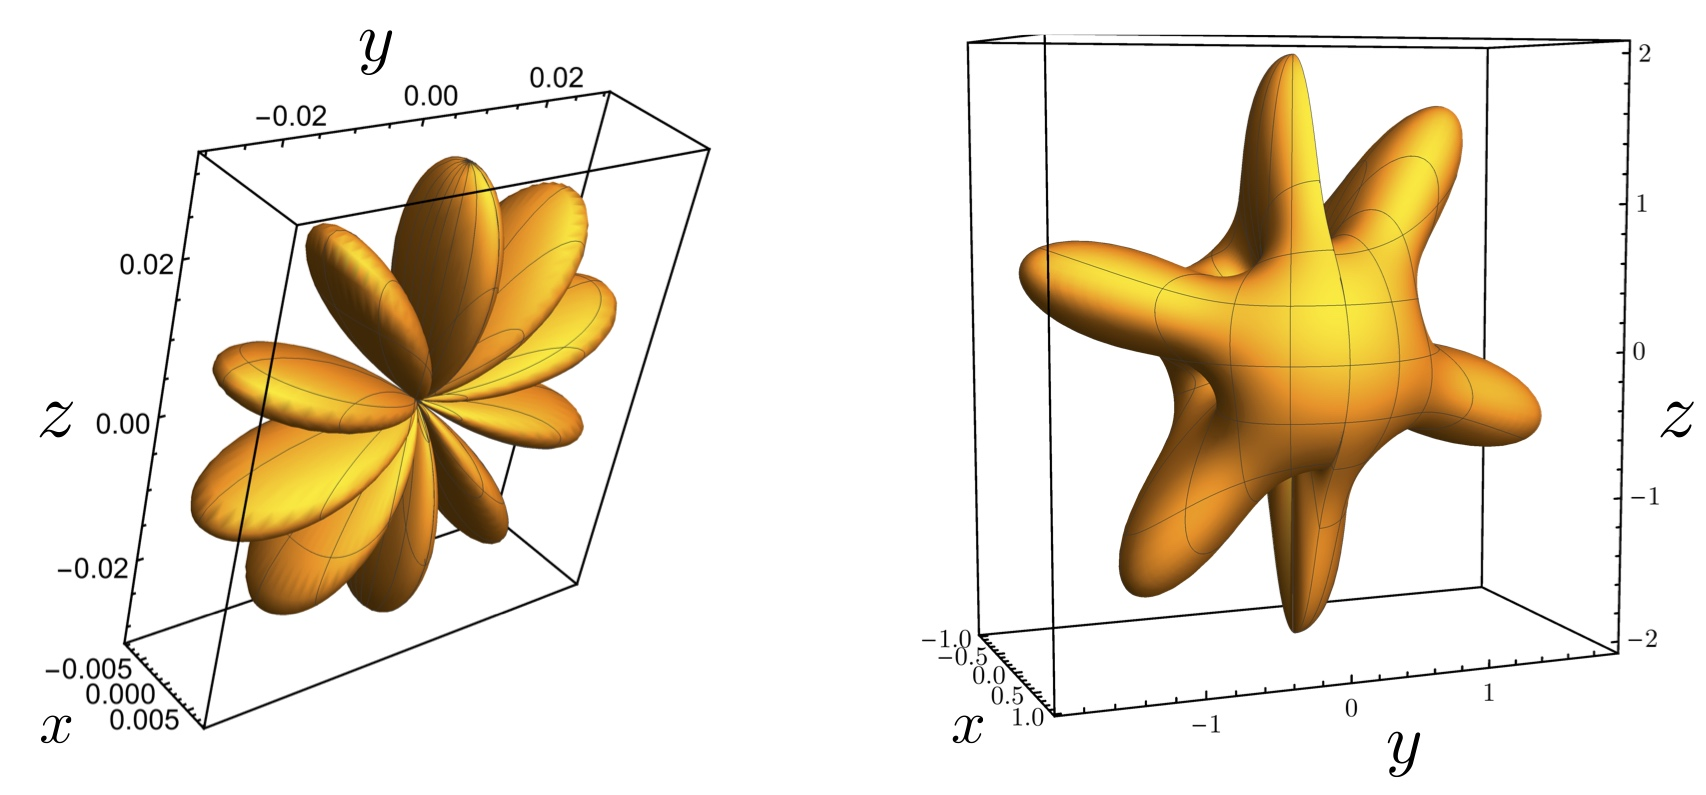
\includegraphics[width=\columnwidth]{experimentalQSE-Insieme.jpg}
    \caption{Spherical polar plot of the interference term $-\text{Re}[q_+(5/2,\alpha,\beta)q^*_-(5/2,\alpha,\beta)]$ in the $Q_2(\alpha,\beta)$ function.}
    \label{fig:expQWs:SCS_plots}
\end{figure}



\section{Conclusions}
\label{sec:expQWs:conclusions}

In this chapter we provided an experimental demonstration of the state engineering protocol given in~\cref{chapter:quantum_walks}. The QW dynamics were implemented with a photonics apparatus using \ac{OAM} and polarisation as the degrees of freedom of the walker.
More specifically, we implemented a five-step \ac{QW} with full control on the preparation, choice of coin operations, and detection stages. To showcase the effectiveness of the protocol, we demonstrated the synthesis of different classes of states.
Our results reinforce the idea that numerical optimisation complementing a complex \ac{QW} dynamics is effective for high-dimensional state engineering.
% A natural generalisation of this novel paradigm could be the engineering in the multipartite scenario, exploiting quantum correlations between multiple walkers. Regarding the research of the coin, further improvements of our approach can be envisaged by identifying appropriate routines to optimize the state engineering process in the presence of actual experimental imperfections.
% To this end, machine learning algorithms can be a promising add-on to our numerical optimisation approach to adapt the coin operators to a given experimental implementation.


%!TEX root =./Thesis.tex

\chapter{Vector vortex beam recognition}
\label{chapter:ML_VVBs}

We show in this chapter a method to classify generated states with nontrivial orbital angular momentum structure, using~\acf{ML} techniques. We use a similar experimental apparatus as the one presented in~\cref{chapter:experimental_engineering_qudits} to generate the states.

\tmpHeading{ML and structured light}
\acf{ML} has recently emerged as a versatile toolbox to tackle a variety of tasks arising in experimental platforms. It has, in particular, proven useful to characterise quantum protocols and dynamics~\cite{carrasquilla2019reconstructing,giordani2018experimental, agresti2019pattern,lumino2018experimental,rocchetto2019experimental,butler2018machine,fischer2006predicting,melnikov2018active,wang2017experimental}\highlight{more refs?}.
In the context of structured light, \acfp{NN} have been used to classify \ac{OAM} states of classical light for long distance free-space communication, even in the presence of environmental turbulence~\cite{krenn2014communication,krenn2016twisted,doster2017machine,park2018demultiplexing,lohani2018turbulence,li2018joint}.
In this chapter, we apply \ac{ML} to characterize experimental \acfp{VVB} generated using the \ac{QW}-based platform presented in~\cref{chapter:experimental_engineering_qudits}~\cite{innocenti2017quantum,giordani2019experimental}.
This approach not requiring neither additional interferometry stabilisation, nor spatial filtering, it provides a robust strategy to decode information stored in \acp{VVB}, and there represents a promising pathway to handle high-dimensional quantum systems. 

\tmpHeading{How is ML been used?}
We leverage both supervised and unsupervised learning techniques. We start by training a \ac{CNN} to classify experimental images belonging to predefined classes of states. This method gives good prediction accuracy, while remaining fairly problem-agnostic and thus useful for diverse applications. However, while providing high prediction accuracy, NN-based methods are difficult to interpret.
We thus also propose an alternative technique based on the joint application of \ac{DR} and supervised learning.
This method provides a geometrical description of the underlying space associated to the experimental data.
While significantly easier to use, such approach gives comparable results to CNN,
at the cost of being more tailored to the specifics of the problem.

\tmpHeading{Our work makes significant steps forward...}
Our work makes significant steps forward with respect to previous endeavours: while~\cite{krenn2014communication,krenn2016twisted,doster2017machine, park2018demultiplexing, lohani2018turbulence, li2018joint} leverage \acp{NN} to process \ac{OAM} states, our work is the first to tackle \acp{VVB}. Moreover, owing to the variety of techniques we deploy, we can address both classification and regression tasks, thus enabling the reconstruction of the input states in relevant cases of structured light beams.
Our findings demonstrate the reliability of a broader class of ML methods, providing novel recognition methods to deal with \ac{VVB}, which are a building block for several information protocols with high-dimensional systems.


\begin{figure}[tb]
	\centering
   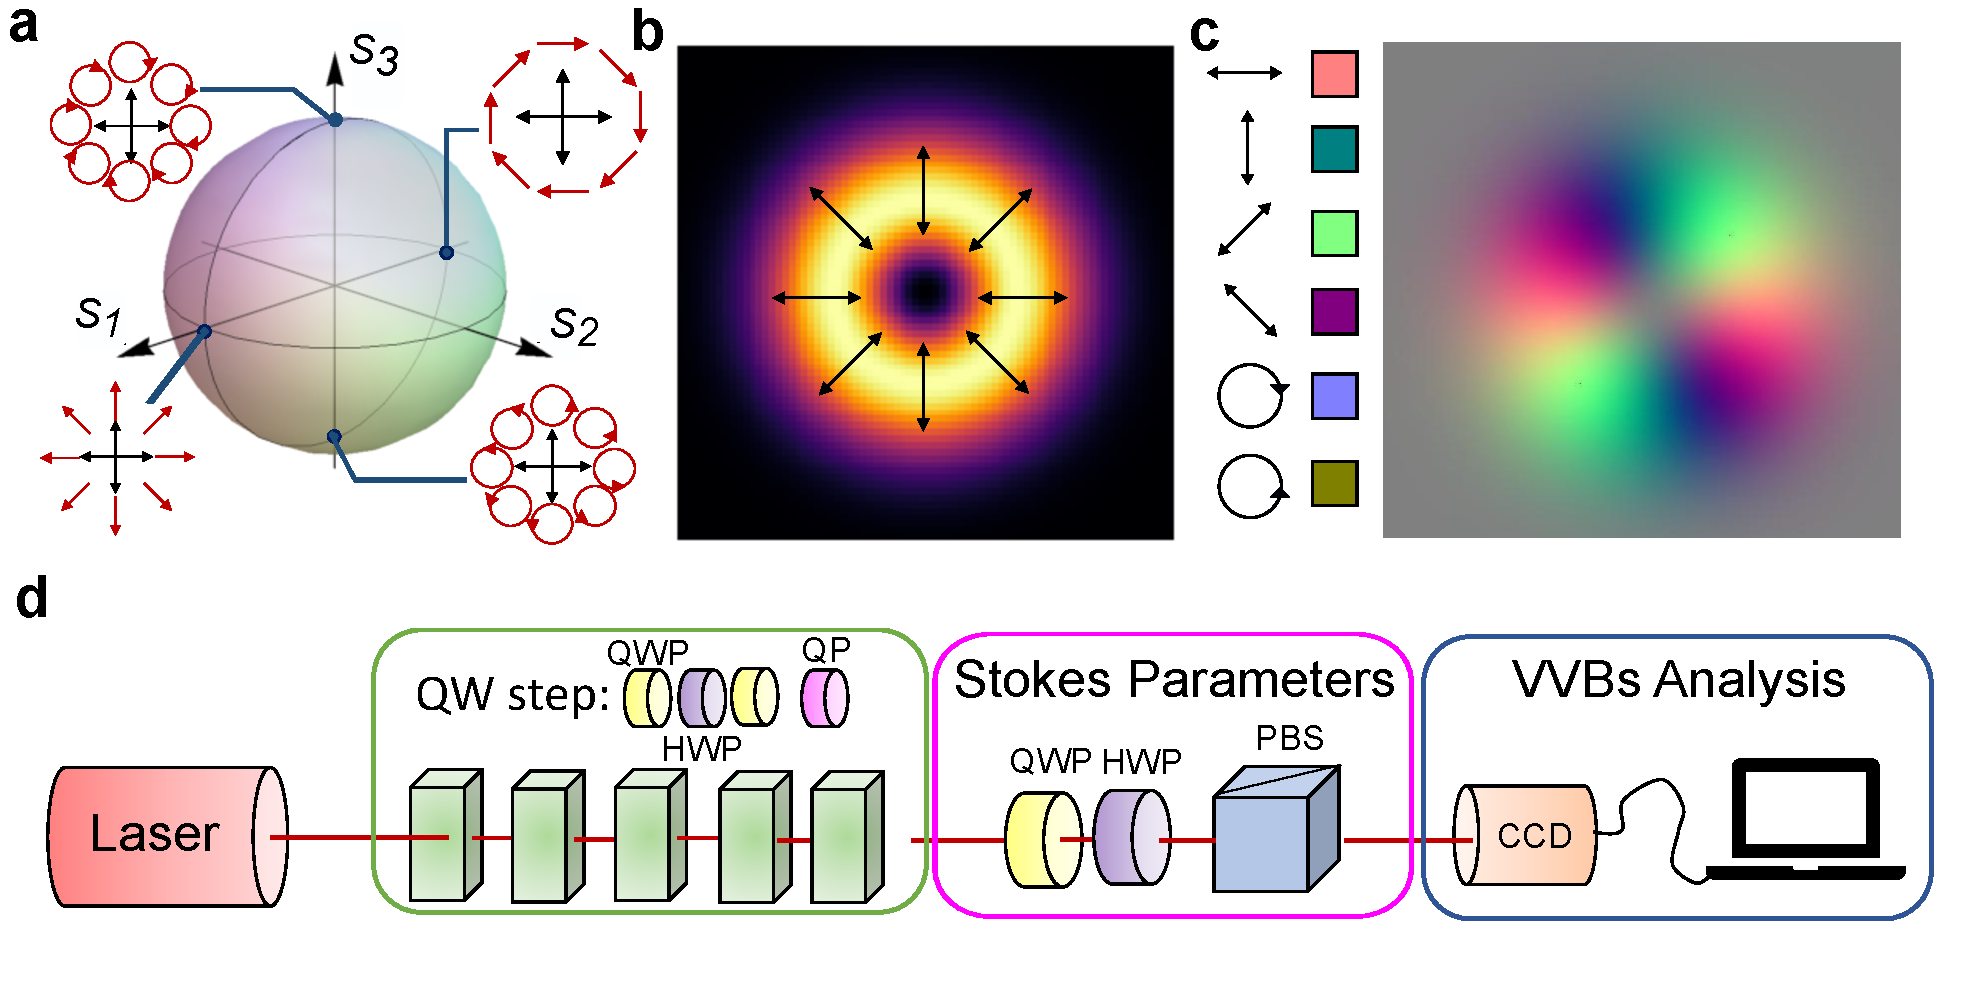
\includegraphics[width=0.8\textwidth]{VVBs-Fig1.pdf}
    \caption{
    	\textbf{(a)} High-order Poincar\'e sphere representation for $|m_{1,2}|=1$. Each point on the sphere surface corresponds to specific polarisation patterns. 
	    \textbf{(b)} A radially polarized \ac{VVB}: at a given point in the trasversal plane the polarisation vector has a different orientation. The Stokes parameters vary accordingly in the plane.
	    \textbf{(c)} Colour encoding of the polarisation pattern. 
	    The legend reports the correspondence between colours and the various polarisations.
	    On the right we have the resulting colour pattern for the VVB in panel {\bf b}.
	    Grey colour corresponds to unpolarised light.
	    \textbf{(d)} Experimental apparatus for the generation of \acp{VVB}. A continuous-wave laser emits a Gaussian beam ${\rm TEM}_{00}$ at $808$ nm. Light undergoes a 5-step quantum walk realized through a sequence of waveplates and QPs.
    	A CCD camera-based detection stage acquires information on the Stokes parameters and the polarisation pattern. Based on the intensity measured at each pixels of the  camera, Stokes parameters are evaluated and converted into RGB-coloured pictures.
    }%
    \label{fig:VVBs:poinc_sphere}
\end{figure}


\section{Experimental generation of Vector Vortex Beams}

\tmpHeading{OAM and LG modes}
\acf{OAM} states of light can be described using \ac{LG} modes.
These are solutions of the Helmholtz equation in the paraxial approximation, indexed by two integer numbers $(m, p)$, with $m$ describing the azimuthal phase structure of the beam, and $p$ its radial intensity profile.
Each \ac{LG} mode carries a set amount of \ac{OAM}, which in the single-photon regime equals $\hbar m$~\cite{allen1992orbital}.

\tmpHeading{What are VVBs?}

\tmpHeading{VVBs}
\acfp{VVB} are obtained by superposing orthogonal polarisations with different \acp{OAM}~\cite{padgett2004lights}.
More specifically, the electric field $\bs{E}_{m_1m_2p}$ of a \ac{VVB} decomposes as the sum of two~\ac{LG} modes with same $p$ and different azimuthal numbers $m_1>m_2$ carried by orthogonal polarisations:
$\bs{E}_{m_1m_2p}=\Vec{e}_L \cos{ \frac{\theta}{2}}\text{ LG$_{m_1p}$} +\Vec{e}_R e^{i \phi} \sin{ \frac{\theta}{2}}\text{ LG$_{m_2p}$}$,
where $\theta\in[0,\pi], \phi\in[0,2\pi]$ and the unit vectors $\Vec{e}_{L,R}$ stand for left and right circular polarisation, respectively.
For the purpose of this work we can ignore the radial number, setting $p=0$.
For any given value of the parameters $(m_1$, $m_2, \theta, \phi)$, the polarisation pattern of a \ac{VVB} can be mapped onto a generalized Poincar\'e sphere (cf.~\cref{fig:VVBs:poinc_sphere}). In particular, we use the higher-order Poincar\'e representation in which the poles represent eigenstates of the total angular momentum but with opposite signs~\cite{milione2011higherorder}.
These polarisation patterns are reconstructed via the \emph{Stokes parameters} $S_{j}~(j=1,2,3)$, obtained by
measuring the output intensities $I_{b_j,1},I_{b_j,2}$ associated to a given choice of polarisation basis $\{b_j \}=\{b_1=( H,V )$, $b_2=( D,A )$, $b_3=( L,R )\}$ as $S_{b_j}=(I_{b_j,1}-I_{b_j,2})/(I_{b_j,1}+I_{b_j,2})$.
%This is a way to characterise a state via its \emph{Stokes parameters} at every point of the transverse %profile.
%To do this, we first measure the output intensities $I_{b_j,1},I_{b_j,2}$ associated to a given choice of %polarisation basis $b_j$, and then compute the value of the corresponding Stokes parameter $S_{b_j}$ as %$S_{b_j}=(I_{b_j,1}-I_{b_j,2})/(I_{b_j,1}+I_{b_j,2})$.
%The canonical choice for the polarisation bases is $b_1=(H,V), b_2=(D,A)$ and $b_3=(L,R)$.
%%
For a \ac{VVB}, the values of $S_j$ depend on the coordinates in the transverse propagation plane~\cite{cardano2012polarization}.

\tmpHeading{VVBs with RGB encoding}
To visualize the polarisation patterns of \acp{VVB}, we use an RGB colour encoding in which the values of $S_j$ are interpreted as strengths of the corresponding colour. In~\cref{fig:VVBs:poinc_sphere}\textbf{b-c} we report an example of such colour encoding for radially polarized \acp{VVB}.
A natural way to generate~\acp{VVB} is using \acp{QP}~\cite{marrucci2006optical,cardano2012polarization}, which are inhomogeneous birefringent plates modifying the OAM of the incoming light conditionally to its polarisation. 
In our scheme, \acp{VVB} are generated via a sequence of polarisation-controlling waveplates interspersing $5$ cascaded QPs (cf.~\cref{fig:VVBs:poinc_sphere}\textbf{d}).
The apparatus implements a discrete-time QW in the angular momentum, where the order of LG modes takes the role of the \emph{walker} and it is changed according to the polarisation state, which embodies the \emph{coin} degree of freedom~\cite{zhang2010implementation,goyal2013implementing,cardano2015quantum,innocenti2017quantum,giordani2019experimental}.
%This apparatus implements a discrete-time QW in the OAM and polarisation degrees of freedom, in which the order of each LG mode takes the role of the \emph{walker}, and the polarisation that of the \emph{coin} degree of freedom
This allows to generate several classes of VVBs with OAM quantum numbers taking odd values in the interval $\{-5,..,5\}$.
We then collect images associated with different \acp{VVB} and use them to train and benchmark our ML-based approaches to classification , as discussed in the next sections.


\tmpHeading{State engineering scheme}
We use the same experimental platform presented in~\cref{chapter:experimental_engineering_qudits}, with $5$ \acp{QP} in cascade that can be interspaced by either \acp{HWP} or \acp{QWP}. 
% The HWPs compensate the polarisation flip operated by the QPs for the generation of higher order \ac{LG} modes. Conversely, the QWP acts on circular polarisations as an Hadamard transformation. 
Using different sets of these waveplates between consecutive QPs, we can generate VVBs corresponding to different pairs $(m_1,m_2)$ of OAM quantum numbers, and parameters $(\theta, \phi)$.
%sof the higher the increases the \ac{OAM} values associated to a \ac{VVB}. Moreover, using quarter waveplates it is possible to generate \acp{VVB} characterized by Laguerre Gauss modes with different azimuthal numbers $m_{1}>m_{2}$.


\tmpHeading{How are images collected?}
The experimental images are collected using a \ac{CCD} with a resolution of $1360 \times 1024$. 
However, we note that a resolution of $128 \times 128$ is already sufficient for the classification tasks we consider. Indeed, the training stage of the algorithms can be significantly speeds up by coarse-graining the images via an integration of its sub-blocks without any loss of information. 

\tmpHeading{Stokes parameters}
For each generated \ac{VVB}, we measure the transverse intensity profile corresponding to each of the two outputs associated with each one of the three independent polarisation bases: $b_1=(H,V), b_2=(D,R)$, and $b_3=(L,R)$, where $\ket L\equiv \frac{1}{\sqrt2}(\ket H + \ket V)$, $\ket R\equiv \frac{1}{\sqrt2}(\ket H - \ket V), \ket D\equiv \frac{1}{\sqrt2}(\ket H + i \ket V), \ket R\equiv \frac{1}{\sqrt2}(\ket H - i \ket V)$.
This amounts, for each generated \ac{VVB}, to acquiring six intensities for each pixel of the \ac{CCD}. This representation is however redundant, as the properties of the VVBs only depend on the relation between the two intensities in each polarisation basis (which, in the single-photon regime, would correspond to the two outcome probabilities).
We therefore represent states using the \emph{higher-order Poincar\'e representation} \cite{milione2011higherorder,cardano2012polarization}. In this representation, each state is mapped into its three \emph{Stokes numbers} $S_{b_j}$, which equal the difference between the two intensities in each choice of polarisation basis:
\begin{equation}
  S_{b_j} = \frac{I_{b_j,1} - I_{b_j,2}}{I_{b_j,1} + I_{b_j,2}},
\end{equation}
where $b_j$ is one of the three canonical polarisation bases, and $I_{b_j,1}, I_{b_j,2}$ are the intensities corresponding to the two possible outcomes when measuring in the basis $b_j$.
In this representation, we therefore associate three real numbers to each each pixel in the \ac{CCD} camera. This means that each detected state is characterised by $128\times128\times3$ real numbers. To visualise these states, we represent the three Stokes numbers $S_{b_j}$ using an RGB colour encoding. In particular, the strengths of the colours red, green and blue are associated with the $S_{1}$, $S_{2}$ and $S_{3}$ parameters,  respectively.
This allows us to map each VVB state into a three-channel coloured image.

For the purpose of the classification algorithms described in~\cref{sec:VVBs:classification,sec:VVBs:dimensionality_reduction,sec:VVBs:SVMs}, each state is represented as a real vector of length $128\times128\times 3$.


\begin{figure}[tb]
	\centering
	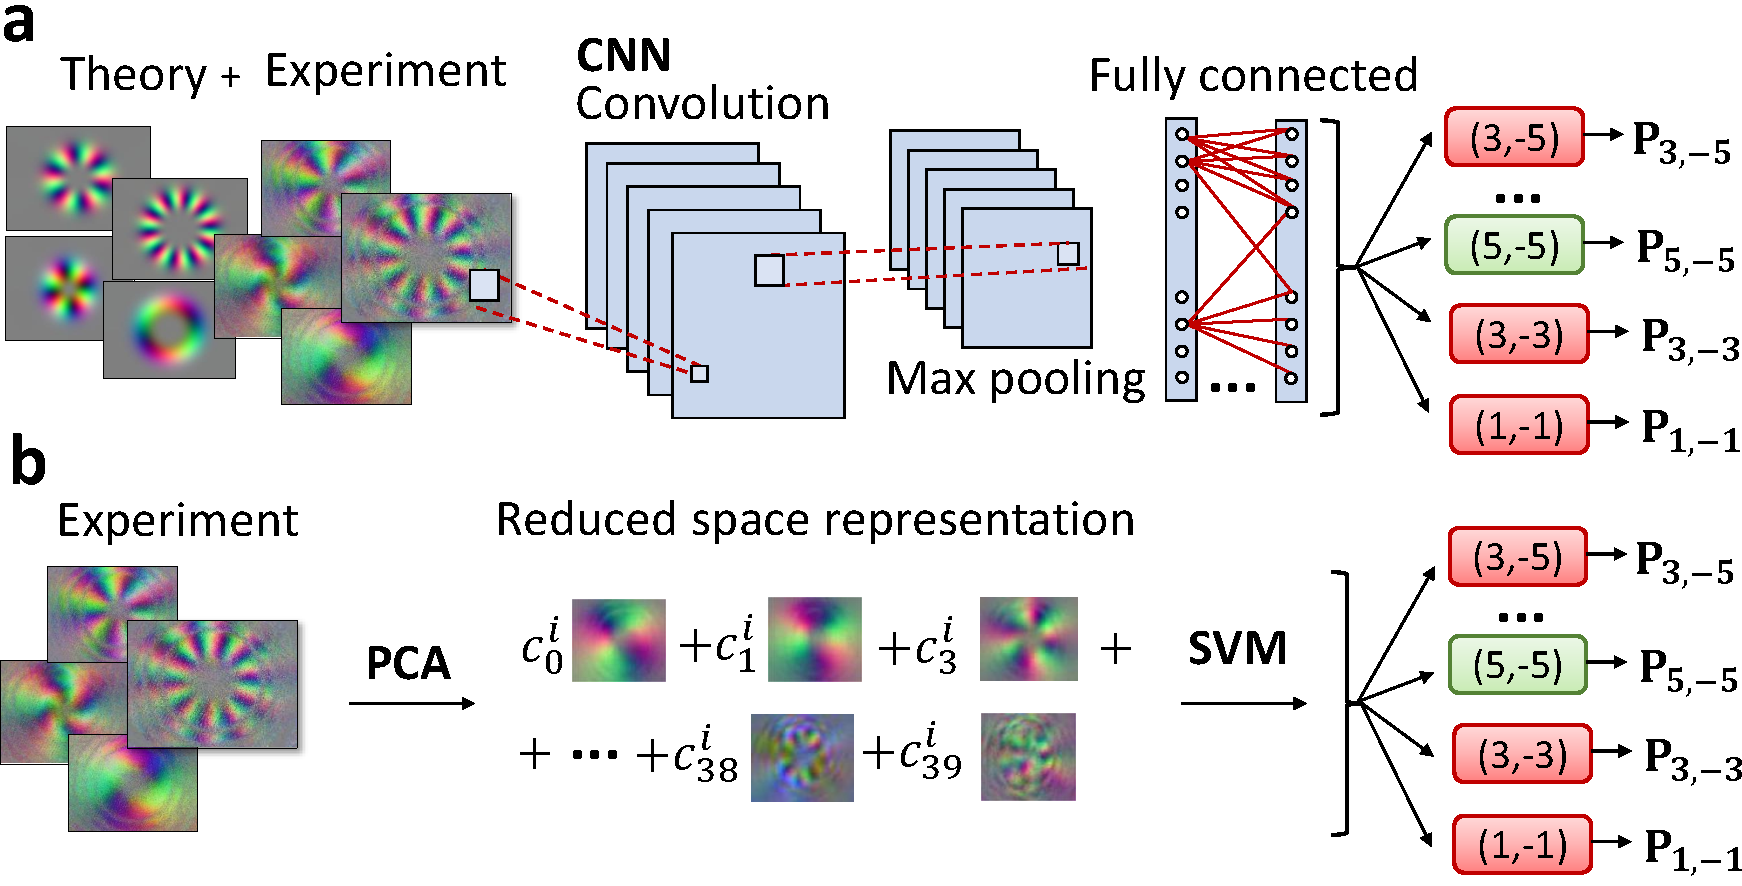
\includegraphics[width=\textwidth]{conc_VVB_2.pdf}
	\caption{
	\textbf{(a)}
	Working principles of \acp{CNN}. The training set consists of a series of simulated images, plus some others collected from the experimental platform.
	\textbf{(b)}
	Classification scheme using linear \ac{PCA}.
	After reducing the dimensionality of the dataset via \ac{PCA}, a linear \ac{SVM} is used to classify experimental images. 
	}
	\label{fig:VVBs:class_techniques}
\end{figure}

\begin{figure}[tb]
    \centering
    \includegraphics[width=0.8\textwidth]{VVBs-Fig3.pdf}
    \caption{
	    \textbf{(a)} Comparison between expected and recorded polarisation patterns for some \acp{VVB} of the ensemble in table, with the corresponding values $(m_1,m_2)$.
	    \textbf{(b)} Scaling of the average accuracy per class when classifying states into one of the $15$ VVB classes,
	    against the fraction of experimental images in the training set. 
	    Inset: best truth table.
	    Rows (columns) stand for the possible $(m_1,m_2)$ pairs (as assigned by the CNN). The matrix elements have been averaged over $100$ experimental images per class.
    }%
    \label{fig:VVBs:resultsCNN}
\end{figure}



\section{Convolutional neural networks}
\label{sec:VVBs:CNNs}

\tmpHeading{What do we use CNNs for?}
We show here how to train a \ac{CNN} to retrieve the parameters $(m_1,m_2)$ characterizing a given VVB from experimentally measured Stokes parameters.
This means to feed the algorithm with input images correspmeasured Stokes parametersonding to one of a number of possible classes of states, and train the network to give as output the corresponding value of the OAM numbers $(m_1,m_2)$.
Moreover, we train the network to recognise the parameters $(\theta,\phi)$ for a given measurement of Stokes parameters, when all the input states have the same OAM numbers $(m_1,m_2)$.

\tmpHeading{What are CNNs?}
\acp{CNN} are translation-invariant deep NNs well-suited for image classification~\cite{lecun2015deep}, to recognise off-centre images and segmented handwritten digits~\cite{simard2003best,ciresan2011flexible},
and for facial recognition tasks~\cite{matsugu2003subject}. 
In their simplest form, \acp{CNN} work by first applying a \emph{convolutional layer}, which consists of a series of nonlinear transformations applied to the input images, followed by a \emph{max-pooling layer}, which downsamples and filters the information extracted by the previous layer. Finally, a fully connected layer functions as a \emph{classifier}, categorizing the information extracted in the previous layers into one of a small number of possible output categories.

\tmpHeading{CNNs more in detail}
We describe here in more detail the structure of the \ac{CNN} used to classify the experimental images.
In a standard \ac{CNN}, the convolution in a particular location $(x,y)$ is obtained by computing the inner product between a $k \times k$ sub region of the input image and a filter of the same size. Repeating this process for each location on the input image, it is possible to obtain an activation map associated to specific features. Typically, more than one filter is used in one convolution layer and $N$ features are extracted.
A max-pooling layer is used immediately after the convolutional layer to reduce the number of parameters. The output of the previous layer are then divided into blocks of size $p \times p$, and the $\max$ function is applied over each block.
Finally, a fully connected layer classifiers the data by determining which features are most correlate to a particular class.
At the beginning, the filters of the features extractors are randomly initialized. Consequently, they are computed via a back-propagation process to optimize the classification of a training set.

\tmpHeading{Categorisation into discrete classes}
The network is first fed with a training set made out of simulated images of \acp{VVB} achievable with a five-step \ac{QW}.
The task is then to discern between $15$ classes, corresponding to the pairs $(m_1,m_2)$ in Fig.~\ref{fig:VVBs:resultsCNN}\textbf{a}.
For each class we generate states with $\theta=\pi/2$ and $\phi\in[0,2\pi]$. The size of the training set is $400$ images per class. Additional $100$ simulated images per class are used to benchmark the performance during training. In these conditions, the network achieves an accuracy of $100\%$. 
We then collect $100$ experimental images per class, to use as new validation set (cf. Fig.~\ref{fig:VVBs:class_techniques}{\bf a}). Fig.~\ref{fig:VVBs:resultsCNN}{\bf a}-{\bf b} shows the mean accuracy per class against the fraction of experimental images gradually inserted in the training set, starting from one consisting of computer-generated images only.
Remarkably, a small increase of the number of experimental images in the training set results in a good accuracy reached by the network (cf. Fig.~\ref{fig:VVBs:resultsCNN}{\bf b}): an average accuracy of $\sim 0.989$ is already obtained when $12.5\%$ of the training set is composed of experimental images.


\tmpHeading{Retrieving the position in the Poincaré sphere}
We use a similar approach to retrieve the position on the Poincaré sphere corresponding to states generated with fixed $(m_1,m_2)$.
We then test the performance of the CNN in the classification of each recorded VVB according to the values $(\theta,\phi)$ for $m_2=-m_1=1$.
To achieve this, the network should discriminate rotations in the polarisation patterns (i.e. changes in $\phi$) and variations in the colour tone (i.e. changes in $\theta$). A drawback of using any type of classifier for this task is that VVBs with $|m_i|\gg1$ display a polarisation pattern whose periodicity decreases as $\frac{2\pi}{|m_1-m_2|}$ (cf. Fig.~\mbox{\ref{fig:VVBs:resultsCNN}}{\bf a})~\cite{fickler2012quantum,dambrosio2013photonic}.
This complicates the recognition of $\phi$, as changes in the phase generate only small rotations of the pattern.
Furthermore, the classification of the VVB on the sphere requires a discretization of $\theta$ and $\phi$, which results in dividing the sphere in sectors. This means that VVBs placed at the borders of these intervals are more difficult to assign to a specific class.
The network is then trained with simulated images corresponding to different positions on the sphere. 
%(that is, different values of $(\theta,\phi)$).
The latter is divided in 26 sectors as follows: $\theta$ is divided in $3$ intervals $\left[k \frac{\pi}{8}, (k+2) \frac{\pi}{8}\right]$ ($k=2n+1$, $n \in \{0,1,2\}$), while $\phi$ is split in the 8 classes $\left[t \frac{\pi}{4}, (t+1) \frac{\pi}{4}\right]$ with $t \in \{0,...,7\} $. The remaining two classes, representing the two poles, correspond to $\theta \in \left[0, \frac{\pi}{8}\right]$ and $ \left[ \frac{7}{8} \pi, \pi\right]$, with no distinction in $\phi$ [cf. Fig. \ref{fig:VVBs:PCAresults}{\bf a}].
We generate $500$ images per class in the training set, and $125$ per class for the validation one. The maximum accuracy  achieved is $\sim 0.90$. This result, which is inferior with respect to what is achieved by only inferring $m_{1,2}$,  confirms the sub-optimality of the method when we had to artificially coarse-grain two continuous parameters.

\tmpHeading{How did we implement the CNN?}
To build and train the \ac{CNN} we used the Python library \emph{Keras}~\cite{chollet2015keras}.
We used a CNN with three feature extractors and one classifier. In each convolution layer we apply $32$ filters of size $3 \times 3 \times 3$ and as activation function is used the Rectified Linear Unit (ReLU). Subsequently, the max function is applied over blocks of size $2 \times 2 \times 3$  in max-pooling layers. %\redComm{(unclear)}. 
The final classification is performed by a fully connected layer which uses a sigmoid activation function. The network training consists of a finite number of epochs each of which composed of $200$ training steps and $100$ validation steps. 


\section{Dimensionality reduction}
\label{sec:VVBs:dimensionality_reduction}

\tmpHeading{What do we use DR for?}
We now present an alternative approach to classify \acp{VVB} from experimental data, leveraging \ac{DR}.
Such algorithms are typically used to obtain efficient representations of large datasets~\cite{cunningham2008dimension,fodor2002survey}.

\subsection{Dimensionality Reduction and Principal Component Analysis}

\tmpHeading{What is DR?}
\acf{DR} stands for a class of algorithms whose goal is to find compact low-dimensional encodings of high-dimensional datasets.

\tmpHeading{Why DR?}
This has several advantages, from easing data visualisation, to improving the efficiency of classification and regression algorithms, which can be used on the reduced representation of the data.
In particular, we employ a linear 
\ac{PCA} algorithm, which works by representing each datapoint as a vector in some high-dimensional space $\RR^n$, and finding the directions in such space that capture the maximum amount of information about the dataset~\cite{jolliffe2011principal,jolliffe2016principal}.
The rationale for using \ac{PCA} in this context is that, although experimental images live in extremely high-dimensional spaces (whose dimension is of the order of the number of pixels in the \ac{CCD} camera), the underlying dimension of the generated \acp{VVB} is typically much lower.
This means that, although the experimental dataset will \emph{a priori} seem like a complicated bundle of high-dimensional vectors, the underlying data is actually characterizable by a small number of parameters. Furthermore, the linearity of the mapping preserves the convexity of the VVB space and thus its geometrical structure. We then expect that the new description for expressing the experimental images in the reduced space provides a synthetic description for capturing the features of VVBs encoded in the measurements (the intensities in three polarisation bases $\{b_j\}$).
This is a form of \emph{unsupervised} learning, as we gain useful information about the origin of the images are inferred without feeding the algorithm with any knowledge of the underlying process.

\tmpHeading{DR and PCA}
The main idea behind dimensionality reduction algorithms is to reduce the dimensionality of a dataset while retaining as much of its important features as possible. More specifically, we use linear \ac{PCA}~\cite{jolliffe2016principal}. The goal of this dimensionality reduction algorithm is to find the directions upon which projecting the dataset vectors gives the maximum amount of variance. More specifically, if the dataset is comprised of $N$ (real) vectors of length $M$, defining the \emph{data matrix} $\bs X$ as the $N\times M$ matrix whose $i$-th row is the $i$-th dataset vector, \ac{PCA} consists in finding the vectors $\bs a\in\RR^{M}$ that maximise the variance of $\bs X\bs a$. This turns out to be equivalent to diagonalising $\bs S\equiv \tilde{\bs X}^T\tilde{\bs X}/(N-1)$, where $\tilde{\bs X}$ is the \emph{centered data matrix}, which is equal to $\bs X$ modulo each of its columns shifted in order to average to zero.
The first $k$ \emph{principal components} found by \ac{PCA} are then the $k$ eigenvectors of $\bs S$ corresponding to the largest $k$ eigenvalues.
Note that these principal components are themselves vectors of the same ``type'' as the data vectors. This means that \ac{PCA} effectively generates a set of data vectors which ``optimally represent'' the information content of the given dataset.

\tmpHeading{For example...}
For example, in our case, each row of $\bs X$ is a vector of length $128\times128\times3$ containing the Stokes parameters $S_{b_1}, S_{b_2}, S_{b_3}$ for each pixel of the camera.
Because each image corresponds to such a vector, and vice versa each such vector corresponds to the image of a \ac{VVB}, we can represent the principal components found by \ac{PCA} again in the form of images, which allows us to gain some intuition into the type of principal components that optimally represent the data according to \ac{PCA}.

\subsection{Retrieving states from probabilities}

\tmpHeading{Linearity of the states $\to$ probabilities mapping}
Let now $\rho$ be the density matrix characterizing a \ac{VVB} state. The corresponding image can be associated to the set of real numbers $p_k=(\mathcal U\rho\mathcal U^\dagger)_{kk}$ with $\mathcal U$ the unitary operator that performs the basis change from the \ac{OAM} to the position basis. In other words, $\rho$ describes the state in the OAM-polarisation basis, which is the basis in which the generated states are efficiently described, whereas $\mathcal U\rho\mathcal U^\dagger$ describes the same state in the position basis, which is the one in which the CCD camera operates on.
The set of detected probabilities is then given by~\footnote{It should be noted that, while here we use a formalism and vocabulary evocative of quantum states, the states actually used in the experiment are classical. This in now way impacts the formal description of the protocol, and the only thing that should change when the states used are classical is that the probabilities $\bs p$ should be reinterpreted as intensities.}
$\bs p=\on{diag}(\mathcal U\rho\mathcal U^\dagger)\equiv\Psi(\rho)$,
where $\Psi$ is defined as the linear map that sends $\rho$ to the set of measured probabilities $\bs p$.
Crucially, the linearity of $\Psi$ implies that it preserves the \emph{convexity} of the space of states, and therefore many of its geometrical features.
For example, if we consider the set of states of the form $c_0 \ket{\uparrow,m=m_1} + c_1 \ket{\downarrow,m=m_2}$ with $m_1\neq m_2$, then the associated density matrices will be arranged to form a three-dimensional sphere embedded in the full state space (because these are effectively different states of a single qubit).
Thanks to the linearity of $\Psi$, \emph{the corresponding probabilities $\bs p$ will also be contained in a spherical surface}, up to possible rescaling of the axes.
In other words, the Bloch sphere of the original two-dimensional system is still present, albeit hidden, in the experimental images, embedded into an extremely high-dimensional space.


\begin{figure}[tb]
    \centering
    \includegraphics[width=0.8\linewidth]{VVBs-Fig4.pdf}
    \caption{
		\textbf{(a)} High order Poincar\'e sphere for \acp{VVB} with $|m_{1,2}|=1$. Magenta-coloured parallels (Blue-coloured meridians) mark intervals between consecutive values of $\theta$ ($\phi$). 
		Along a meridian the colours of the pattern vary from the hottest to the coldest one. Along a parallel, the patterns rotate. 
		\textbf{(b)}
		Comparison between experimental and simulated \ac{VVB} images for different angles $(\theta, \phi)$.
		\textbf{(c)}
		Distribution of fidelities obtained comparing each experimental VVBs with its reduced 3D representations given by PCA. Projecting each image onto its first three principal axes and rescaling brings the data (orange points) onto a sphere in 3D, as shown in the inset. The inner (outer) black (semi-transparent) sphere is added for contrast [radius equal to that of the point with smaller (larger) radius].
		\textbf{(d)}
		Average prediction accuracy of a linear \ac{SVM} classifier, trained and tested after applying linear DR to the data, against the number of reduced dimensions $n_c$.
		For each of the 15 classes (cf.~\cref{fig:VVBs:resultsCNN}a) in which the experimental dataset was divided, we show in the inset the true-table. 
    }%
    \label{fig:VVBs:PCAresults}
\end{figure}


\subsection{Results}

\tmpHeading{PCA applied to experimental data}
As a notable example, we apply these observations to VVBs with $m_2=-m_1=1$, which can be pictured as lying on a sphere, in the higher-order Poincaré representation. 
of the form $c_0 \ket{L,m=1} + c_1 \ket{R, m=-1}$ with $\abs{c_0}^2+|c_1|^2=1$.
The inclusion of only two orthogonal basis states makes these states effectively equivalent to a single qubit. 
Indeed, \ac{PCA} applied to the experimental dataset of~\cref{fig:VVBs:PCAresults}\textbf{b}, 
reveals that only three directions capture most of the information content of the images. Projecting the images along these three principal components, we recover that the data is arranged in the form of a three-dimensional sphere embedded in the high-dimensional space of experimental (cf. inset of~\cref{fig:VVBs:PCAresults}\textbf{c}).
Remarkably, this was not obvious from the experimental dataset alone, but was easily found via \ac{DR}. This result highlights the potential of \ac{DR} to  reveal features of the underlying states generating a given experimental dataset, also in the presence of experimental noisy conditions.
To assess the accuracy of such reconstruction, we compute the average fidelity $\mathcal F_{\text{avg}}$ between the expected state and the one found by our analysis with PCA. As shown in the histogram of Fig.~\ref{fig:VVBs:PCAresults}c,  this is found to be $\mathcal F_{\text{avg}}\sim0.96$ (standard deviation $\sim0.01$), thus certifying the quality of the reconstruction.

\begin{figure}[tb]
  \centering
  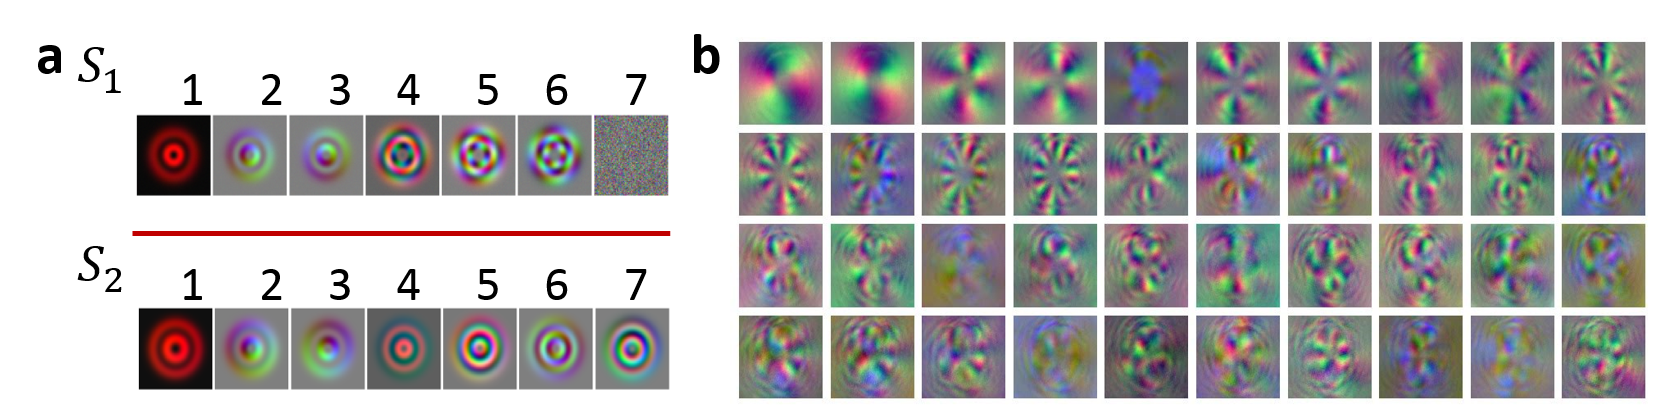
\includegraphics[width=0.98\textwidth]{S1_fig.png}
  \caption{
      \textbf{a,}
       Principal components obtained using PCA on simulated datasets of noisy VVB. The first (second) row shows the first seven principal components obtained on the dataset $\mathcal S_1$ ($\mathcal S_2$). 
       The first 6 (all 7) components correspond to non-vanishing singular values.
       \textbf{b,} First 40 principal components individuated in the experimental dataset corresponding to the 15 classes labelled by $(m_1,m_2)$, discussed in the main text.%
    }
    \label{fig:S1}
\end{figure}


\tmpHeading{Toy examples of application of PCA to VVBs}
To see the usefulness of these ideas to understand the type of states generated by a given apparatus, we consider here two examples of applications of \ac{PCA} for different types of input states. 
In all of these cases, \ac{PCA} is applied without any previous knowledge of the type of states that underly the observed experimental images, and is therefore to be considered a type of \emph{unsupervised learning}.
Consider a simulated set of images corresponding to VVBs of the form
$c_1\ket{L,m=1}+c_2\ket{R,m=2}$ and
$c_1\ket{L,m=1}+c_2\ket{R,m=4}$, where the coefficients $c_i$ are sampled uniformly at random from the set of $c_{1},c_2\in\mathbb{C}$  such that $|c_1|^2+|c_2|^2=1$ (\emph{i.e.} uniformly sampled on the Bloch sphere).
Applying PCA to this dataset, we find six non-vanishing singular values, whose associated principal components are given in Fig.~\ref{fig:S1}a.
This is consistent with the dimension of the subspace  spanned by states of the form $\mathcal S_1=\{c_1\ket{L,1}+c_2\ket{R,2}, c_3\ket{L,1}+c_4\ket{R,4}\}$,  as the set of corresponding density matrices is spanned by the six orthogonal matrices
$X^{(1,2)}, X^{(1,4)}, Y^{(1,2)},Y^{(1,4)},Z^{(1,2)}\pm Z^{(1,4)}$, where $X^{(i,j)}=\ketbra{i}{j}+\ketbra{j}{i}$ is the Pauli $X$ matrix acting on the $(i,j)$ subspace, and similarly for $Y^{(i,j)}$ and $Z^{(i,j)}$.
On the other hand, if the dataset under consideration consists of states of the form $\mathcal S_2=\{c_1\ket{L,1}+c_2\ket{R,2}, c_3\ket{L,3}+c_4\ket{R,4}\}$, then \ac{PCA} finds \emph{seven} principal components associated with non-vanishing singular values (see Fig.~\ref{fig:S1}a).
This is consistent with the underlying state space being spanned by the seven orthogonal Hermitians:
\begin{equation}
\begin{gathered}
    X^{(1,2)}, \,\, X^{(3,4)}, \,\,
    Y^{(1,2)}, \,\, Y^{(3,4)}, \\
    Z^{(1,2)},\quad
    -Z^{(1,2)} + 2 Z^{(1,3)}, \\
    -Z^{(1,2)} - Z^{(1,3)} + 3 Z^{(1,4)}.
\end{gathered}
\end{equation}
These matrices can be obtained by direct analysis of the type of states contained in $\mathcal S_2$ and then finding a set of orthogonal Hermitian matrices generating the corresponding set of density matrices.
It is worth noting how this method provides a quick and easy way to gain useful information about the dimensionality of generated states, as well as about other properties such as specific symmetries, which, as shown in~\cref{fig:S1}, are often picked up by the principal components.


\section{Support vector machines}
\label{sec:VVBs:SVMs}

\subsection{What are they}


\subsection{How do we use them?}

\tmpHeading{SVMs after PCA}
We now show how the reduced representations provided by \ac{PCA} can function as starting point to train a classifier with accuracy comparable with the \ac{CNN}, whilst requiring a significantly reduced amount of computational resources.
More precisely, we use as classifiers linear multiclass \acp{SVM}~\cite{hearst1998support,shawe2000support}. These supervised learning algorithms categorize data by finding the hyperplane that optimally separates the training dataset in accordance with the corresponding labels.
We use here in particular a \emph{linear}, multiclass \ac{SVM}, whose goal is to find hyperplanes in the feature space that optimally separate the datapoints corresponding to different classes.
During the training phase, a set of training experimental images is used to find the separating hyperplanes, which can then be used to classify new experimental images.

\tmpHeading{What do we use the SVMs for?}
As done for the \ac{CNN}, we consider the task of classifying experimental dataset of VVBs. We train a \ac{SVM} on the reduced space obtained via \ac{PCA}, applied to the experimental dataset reported in~\cref{fig:VVBs:resultsCNN}\textbf{a}. This stage significantly improves the training cost of the classifier since the latter will work on a synthesised description of the high-dimensional space of images in which the features of each class can be easily recognised.
This not only significantly speeds up training the classifier, but also makes for a more robust classification, thanks to the property of dimensionality reduction algorithms to weed out statistical and experimental noise.
What's more, the geometrical picture offered by the reduced representation tells us when we should expect this classification to be accurate: \ac{PCA} effectively retrieves the description of the states in the generalized Bloch representation, therefore the classification will give good results whenever the states are linearly separated in state space.


\tmpHeading{What is used for the training?}
The~\ac{SVM} was trained on half of the experimental data, with the other half used to test the resulting accuracy. A breakdown of the classification performance is reported in the inset of~\cref{fig:VVBs:PCAresults}\textbf{d}, where we detail how the images belonging to each class were classified.

\tmpHeading{What kind of SVM do we use?}
We used here a \emph{linear} SVM, instead of a commonly used SVM with RBF kernel, because we found it to perform better: an RBF kernel was found to give, in our case, an average accuracy of only $\sim94\%$.
Furthermore, in~\cref{fig:VVBs:PCAresults}\textbf{d} we highlight how the average overall accuracy depends on the dimension of the reduced representation: $\sim 25$ dimensions are already sufficient to get good average accuracies.

\subsection{Results}

The average classification accuracy achieved on images not included in the training set is $\sim 98 \%$. This result confirms that the description provided by \ac{PCA} is sufficient to capture the important features of the generated states, thus allowing for a dramatically more efficient classification scheme.


\section{Conclusions}
\label{sec:VVBs:conclusions}

We presented a new approach to classify \acp{VVB} leveraging ML techniques. We demonstrated how the use of inference strategies based on CNNs and PCA (enhanced by SVMs) allows to extract efficiently properties of high-dimensional photonic \ac{VVB} systems.
In particular, DR was used to obtain a deeper understanding of the underlying geometrical properties of the experimentally generated states, without requiring prior knowledge about the physics of the generation apparatus.
% this is not quite right
By embedding a variety of {\ac{ML}} algorithms into our experimental pipeline, the task of characterising structured light is made significantly broader in the methods, ranging from supervised to unsupervised learning, and more flexible in the applications, classification and regression tasks.
%
%Then, the investigation of different techniques in the ML field has provided a more general framework for the characterization of structured light. 
% 
While paving the way to further experimental validations -- potentially also in experimental settings that do not rely on optical networks -- we believe that numerous tasks of relevance to modern photonics could benefit from introducing similar {\ac{ML}} ideas into their characterization protocols. These techniques can prove to be useful add-on to tasks ranging from the design of automatized approaches to the characterization of experimental platforms and experiments, to the provision of solutions to OAM demultiplexing in the context of classical and quantum communication and, more generally, for the use of structured light in quantum technologies.

\textit{Note--} During the reviewing process of this manuscript, the authors
became aware of a related work~\cite{liu2019superhighresolution} addressing a similar topic.


%!TEX root = ./Thesis.tex

\clearpage
\phantomsection
\addcontentsline{toc}{chapter}{Bibliography}

% \bibliographystyle{IEEEtran} % IEEE bibliographic/citation style.
% %\bibliography{IEEEabrv,Thesis}
% \bibliography{IEEEfull,Thesis}
\newrefcontext[sorting=nty]
\printbibliography


\end{document}
